
%DIF LATEXDIFF DIFFERENCE FILE
%DIF DEL out_old.tex   Mon Oct  9 10:58:49 2017
%DIF ADD out_new.tex   Mon Oct  9 18:06:36 2017
%% bare_jrnl.tex
%% V1.4b
%% 2015/08/26
%% by Michael Shell
%% see http://www.michaelshell.org/
%% for current contact information.
%%
%% This is a skeleton file demonstrating the use of IEEEtran.cls
%% (requires IEEEtran.cls version 1.8b or later) with an IEEE
%% journal paper.
%%
%% Support sites:
%% http://www.michaelshell.org/tex/ieeetran/
%% http://www.ctan.org/pkg/ieeetran
%% and
%% http://www.ieee.org/

%%*************************************************************************
%% Legal Notice:
%% This code is offered as-is without any warranty either expressed or
%% implied; without even the implied warranty of MERCHANTABILITY or
%% FITNESS FOR A PARTICULAR PURPOSE! 
%% User assumes all risk.
%% In no event shall the IEEE or any contributor to this code be liable for
%% any damages or losses, including, but not limited to, incidental,
%% consequential, or any other damages, resulting from the use or misuse
%% of any information contained here.
%%
%% All comments are the opinions of their respective authors and are not
%% necessarily endorsed by the IEEE.
%%
%% This work is distributed under the LaTeX Project Public License (LPPL)
%% ( http://www.latex-project.org/ ) version 1.3, and may be freely used,
%% distributed and modified. A copy of the LPPL, version 1.3, is included
%% in the base LaTeX documentation of all distributions of LaTeX released
%% 2003/12/01 or later.
%% Retain all contribution notices and credits.
%% ** Modified files should be clearly indicated as such, including  **
%% ** renaming them and changing author support contact information. **
%%*************************************************************************


% *** Authors should verify (and, if needed, correct) their LaTeX system  ***
% *** with the testflow diagnostic prior to trusting their LaTeX platform ***
% *** with production work. The IEEE's font choices and paper sizes can   ***
% *** trigger bugs that do not appear when using other class files.       ***                          ***
% The testflow support page is at:
% http://www.michaelshell.org/tex/testflow/



\documentclass[journal]{IEEEtran}
%


%~ \setcounter{secnumdepth}{3}
\usepackage{moreverb,url}
\usepackage{makeidx}         % allows index generation
\usepackage[percent]{overpic}
\usepackage{array} 
\usepackage{algorithm}
\usepackage[noend]{algpseudocode}
\usepackage{listings}
\usepackage{color}
\usepackage{bm}
\usepackage{booktabs}
\usepackage{multirow}
\usepackage[table]{xcolor}
\usepackage{amsfonts}
\usepackage{amsmath}
\usepackage[Symbol]{upgreek}

\newcommand{\fratop}[2]{\genfrac{}{}{0pt}{}{#1}{#2}}
\newcommand{\mx}[1]{\mathbf{\bm{#1}}} 				% Matrix symbol
\newcommand{\vc}[1]{\mathbf{\bm{#1}}} 					% Vector symbol
\newcommand{\degree}{\ensuremath{^\circ}}				% define the degree symbol
\newcommand{\pder}[2]{\frac{\partial#1}{\partial#2}}		% partial derivative
\newcommand{\ppder}[2]{\frac{\partial^2 #1}{\partial#2^2}}		% second partial derivative
\newcommand{\refframe}[1]{\mbox{\textless#1\textgreater}}	% to denote a reference frame
%\DeclareMathOperator*{\lexmin}{\text{lex}\!\min}			% lexmin
\DeclareMathOperator*{\argmin}{\arg\!\min}				% argmin
\DeclareMathOperator*{\argmax}{\arg\!\max}				% argmax
\DeclareMathOperator*{\st}{subject\,to}					% subject to
\DeclareMathOperator*{\minimize}{minimize}				% 
\DeclareMathOperator*{\maximize}{maximize}				% 
\DeclareMathOperator*{\find}{find}						% 
\DeclareMathOperator*{\dif}{\mathrm{d}}					% d
\DeclareMathOperator*{\half}{\frac{1}{2}}					% one half
\newcommand{\equilibriumfeasibility}[0]{\glslink{equilibrium feasible}{\textit{equilibrium feasibility}}}	% matrix
\newcommand{\contactreachability}{\textit{contact reachability}}	% matrix
\newcommand{\mat}[1]{\ensuremath{\begin{bmatrix}#1\end{bmatrix}}}	% matrix
\newcommand{\rank}[1]{\text{rank}(#1)}							% rank
\newcommand{\diag}[1]{\text{diag}(#1)}							% diag
\newcommand{\x}{\ensuremath{\times}}
\newcommand{\spac}{\ensuremath{\quad}}						% alias for space in math environment
\newcommand{\dx}[0]{\ensuremath{\delta x}}					% dx
\newcommand{\du}[0]{\ensuremath{\delta u}}					% du
\newcommand{\DX}[0]{\ensuremath{\Delta X}}						% DX
\newcommand{\DU}[0]{\ensuremath{\Delta U}}						% DU
\newcommand{\T}[0]{\ensuremath{\top}}							% transpose symbol
\newcommand{\pinv}[0]{\ensuremath{\dagger}}					% pseudoinverse symbol
\newcommand{\Rv}[1]{\ensuremath{\mathbb{R}^{#1}}}				% set of real-valued vectors
\newcommand{\R}[2]{\ensuremath{\mathbb{R}^{#1\times #2}}}		% set of real-valued matrices
\newcommand{\Spd}[1]{\ensuremath{\mathbb{S}_+^{#1}}}			% set of symmetric positive-definite matrices
\newcommand{\card}[1]{\ensuremath{\left\vert{#1}\right\vert}}			% cardinality of a set
\DeclareMathOperator{\Tr}{Tr}							% trace
\newcommand{\Expect}{{\rm I\kern-.3em E}}				% expectation
\newcommand{\Normal}{\mathcal{N}}					% normal distribution
\newcommand{\Prob}[1]{\text{P}(#1)}						% probability

\newcommand{\Y}{\ensuremath{\mathcal{Y}}}					% 
\newcommand{\Yin}{\ensuremath{\mathcal{Y}_{in}}}					% 
\newcommand{\Yout}{\ensuremath{\mathcal{Y}_{out}}}					% 

%\algnewcommand{\algorithmicgoto}{\textbf{go to}}%
%%\algnewcommand{\Goto}[1]{\algorithmicgoto~\ref{#1}}%
%\algnewcommand{\Goto}{\algorithmicgoto\xspace}%
%\algnewcommand{\Label}{\State\unskip}

\newenvironment{definition}[1][Definition]{\begin{trivlist}
\item[\hskip \labelsep {\bfseries #1}]}{\end{trivlist}}

\newcommand{\commentt}[2]{\textcolor{#1}{\textbf{\textit{[#2]}}}} 	% make sure no comments left in the paper
%\newcommand{\commentt}[2]{}							% using this line rather than the previous one you remove all comments
\newcommand{\adnote}[1]{\commentt{blue}{AD: #1}}
\newcommand{\nmnote}[1]{\commentt{OliveGreen}{NM: #1}}

% Another method to track changes
% Examples of usage:
% - This is \added[id=per,remark={we need this}]{new} text.
% - This is \deleted[id=per,remark=obsolete]{unnecessary}text.
% - This is \replaced[id=per]{nice}{bad} text.
% To print the list of change use: \listofchanges
\usepackage{changes}	% use this for the working version
%\usepackage[final]{changes} % use this for the final version
\definechangesauthor[name={Andrea Del Prete}, color=orange]{adp}
\newcommand{\deladp}[1]{\deleted[id=adp]{#1}}
\newcommand{\addadp}[1]{\added[id=adp]{#1}}
\newcommand{\repadp}[2]{\replaced[id=adp]{#1}{#2}}
\definechangesauthor[name={Steve Tonneau}, color=blue]{st}
\newcommand{\delst}[1]{\deleted[id=st]{#1}}
\newcommand{\addst}[1]{\added[id=st]{#1}}
\newcommand{\repst}[2]{\replaced[id=st]{#1}{#2}}
\newcommand{\gls}[1]{\textit{#1}}
\newcommand{\glslink}[2]{{#2}}

%~ \usepackage[colorlinks,bookmarksopen,bookmarksnumbered,citecolor=red,urlcolor=red,draft]{hyperref}
\usepackage[colorlinks,bookmarksopen,bookmarksnumbered,citecolor=red,urlcolor=red]{hyperref}
%~ \usepackage{glossaries}

% If IEEEtran.cls has not been installed into the LaTeX system files,
% manually specify the path to it like:
% \documentclass[journal]{../sty/IEEEtran}

%DIF 156-182d156
%DIF < %% \addtolength{\oddsidemargin}{-.6in}
%DIF < %% \linespread{1.5}
%DIF < %% \addtolength{\textwidth}{-1.5in}
%DIF < %DIF PREAMBLE EXTENSION ADDED BY LATEXDIFF
%DIF < %DIF UNDERLINE PREAMBLE %DIF PREAMBLE
%DIF < \RequirePackage[normalem]{ulem} %DIF PREAMBLE
%DIF < \RequirePackage{color}\definecolor{RED}{rgb}{1,0,0}\definecolor{BLUE}{rgb}{0,0,1} %DIF PREAMBLE
%DIF < \providecommand{\DIFaddtex}[1]{{\protect\color{blue}\uwave{#1}}} %DIF PREAMBLE
%DIF < \providecommand{\DIFdeltex}[1]{{\protect\color{red}\sout{#1}}}                      %DIF PREAMBLE
%DIF < %DIF SAFE PREAMBLE %DIF PREAMBLE
%DIF < \providecommand{\DIFaddbegin}{} %DIF PREAMBLE
%DIF < \providecommand{\DIFaddend}{} %DIF PREAMBLE
%DIF < \providecommand{\DIFdelbegin}{} %DIF PREAMBLE
%DIF < \providecommand{\DIFdelend}{} %DIF PREAMBLE
%DIF < %DIF FLOATSAFE PREAMBLE %DIF PREAMBLE
%DIF < \providecommand{\DIFaddFL}[1]{\DIFadd{#1}} %DIF PREAMBLE
%DIF < \providecommand{\DIFdelFL}[1]{\DIFdel{#1}} %DIF PREAMBLE
%DIF < \providecommand{\DIFaddbeginFL}{} %DIF PREAMBLE
%DIF < \providecommand{\DIFaddendFL}{} %DIF PREAMBLE
%DIF < \providecommand{\DIFdelbeginFL}{} %DIF PREAMBLE
%DIF < \providecommand{\DIFdelendFL}{} %DIF PREAMBLE
%DIF < %DIF END PREAMBLE EXTENSION ADDED BY LATEXDIFF
%DIF < %DIF PREAMBLE EXTENSION ADDED BY LATEXDIFF
%DIF < %DIF HYPERREF PREAMBLE %DIF PREAMBLE
%DIF < \providecommand{\DIFadd}[1]{\texorpdfstring{\DIFaddtex{#1}}{#1}} %DIF PREAMBLE
%DIF < \providecommand{\DIFdel}[1]{\texorpdfstring{\DIFdeltex{#1}}{}} %DIF PREAMBLE
%DIF < %DIF END PREAMBLE EXTENSION ADDED BY LATEXDIFF
%DIF -------




% Some very useful LaTeX packages include:
% (uncomment the ones you want to load)


% *** MISC UTILITY PACKAGES ***
%
%\usepackage{ifpdf}
% Heiko Oberdiek's ifpdf.sty is very useful if you need conditional
% compilation based on whether the output is pdf or dvi.
% usage:
% \ifpdf
%   % pdf code
% \else
%   % dvi code
% \fi
% The latest version of ifpdf.sty can be obtained from:
% http://www.ctan.org/pkg/ifpdf
% Also, note that IEEEtran.cls V1.7 and later provides a builtin
% \ifCLASSINFOpdf conditional that works the same way.
% When switching from latex to pdflatex and vice-versa, the compiler may
% have to be run twice to clear warning/error messages.






% *** CITATION PACKAGES ***
%
%\usepackage{cite}
% cite.sty was written by Donald Arseneau
% V1.6 and later of IEEEtran pre-defines the format of the cite.sty package
% \cite{} output to follow that of the IEEE. Loading the cite package will
% result in citation numbers being automatically sorted and properly
% "compressed/ranged". e.g., [1], [9], [2], [7], [5], [6] without using
% cite.sty will become [1], [2], [5]--[7], [9] using cite.sty. cite.sty's
% \cite will automatically add leading space, if needed. Use cite.sty's
% noadjust option (cite.sty V3.8 and later) if you want to turn this off
% such as if a citation ever needs to be enclosed in parenthesis.
% cite.sty is already installed on most LaTeX systems. Be sure and use
% version 5.0 (2009-03-20) and later if using hyperref.sty.
% The latest version can be obtained at:
% http://www.ctan.org/pkg/cite
% The documentation is contained in the cite.sty file itself.






% *** GRAPHICS RELATED PACKAGES ***
%
\ifCLASSINFOpdf
  % \usepackage[pdftex]{graphicx}
  % declare the path(s) where your graphic files are
  % \graphicspath{{../pdf/}{../jpeg/}}
  % and their extensions so you won't have to specify these with
  % every instance of \includegraphics
  % \DeclareGraphicsExtensions{.pdf,.jpeg,.png}
\else
  % or other class option (dvipsone, dvipdf, if not using dvips). graphicx
  % will default to the driver specified in the system graphics.cfg if no
  % driver is specified.
  % \usepackage[dvips]{graphicx}
  % declare the path(s) where your graphic files are
  % \graphicspath{{../eps/}}
  % and their extensions so you won't have to specify these with
  % every instance of \includegraphics
  % \DeclareGraphicsExtensions{.eps}
\fi
% graphicx was written by David Carlisle and Sebastian Rahtz. It is
% required if you want graphics, photos, etc. graphicx.sty is already
% installed on most LaTeX systems. The latest version and documentation
% can be obtained at: 
% http://www.ctan.org/pkg/graphicx
% Another good source of documentation is "Using Imported Graphics in
% LaTeX2e" by Keith Reckdahl which can be found at:
% http://www.ctan.org/pkg/epslatex
%
% latex, and pdflatex in dvi mode, support graphics in encapsulated
% postscript (.eps) format. pdflatex in pdf mode supports graphics
% in .pdf, .jpeg, .png and .mps (metapost) formats. Users should ensure
% that all non-photo figures use a vector format (.eps, .pdf, .mps) and
% not a bitmapped formats (.jpeg, .png). The IEEE frowns on bitmapped formats
% which can result in "jaggedy"/blurry rendering of lines and letters as
% well as large increases in file sizes.
%
% You can find documentation about the pdfTeX application at:
% http://www.tug.org/applications/pdftex





% *** MATH PACKAGES ***
%
%\usepackage{amsmath}
% A popular package from the American Mathematical Society that provides
% many useful and powerful commands for dealing with mathematics.
%
% Note that the amsmath package sets \interdisplaylinepenalty to 10000
% thus preventing page breaks from occurring within multiline equations. Use:
%\interdisplaylinepenalty=2500
% after loading amsmath to restore such page breaks as IEEEtran.cls normally
% does. amsmath.sty is already installed on most LaTeX systems. The latest
% version and documentation can be obtained at:
% http://www.ctan.org/pkg/amsmath





% *** SPECIALIZED LIST PACKAGES ***
%
%\usepackage{algorithmic}
% algorithmic.sty was written by Peter Williams and Rogerio Brito.
% This package provides an algorithmic environment fo describing algorithms.
% You can use the algorithmic environment in-text or within a figure
% environment to provide for a floating algorithm. Do NOT use the algorithm
% floating environment provided by algorithm.sty (by the same authors) or
% algorithm2e.sty (by Christophe Fiorio) as the IEEE does not use dedicated
% algorithm float types and packages that provide these will not provide
% correct IEEE style captions. The latest version and documentation of
% algorithmic.sty can be obtained at:
% http://www.ctan.org/pkg/algorithms
% Also of interest may be the (relatively newer and more customizable)
% algorithmicx.sty package by Szasz Janos:
% http://www.ctan.org/pkg/algorithmicx




% *** ALIGNMENT PACKAGES ***
%
%\usepackage{array}
% Frank Mittelbach's and David Carlisle's array.sty patches and improves
% the standard LaTeX2e array and tabular environments to provide better
% appearance and additional user controls. As the default LaTeX2e table
% generation code is lacking to the point of almost being broken with
% respect to the quality of the end results, all users are strongly
% advised to use an enhanced (at the very least that provided by array.sty)
% set of table tools. array.sty is already installed on most systems. The
% latest version and documentation can be obtained at:
% http://www.ctan.org/pkg/array


% IEEEtran contains the IEEEeqnarray family of commands that can be used to
% generate multiline equations as well as matrices, tables, etc., of high
% quality.




% *** SUBFIGURE PACKAGES ***
%\ifCLASSOPTIONcompsoc
%  \usepackage[caption=false,font=normalsize,labelfont=sf,textfont=sf]{subfig}
%\else
%  \usepackage[caption=false,font=footnotesize]{subfig}
%\fi
% subfig.sty, written by Steven Douglas Cochran, is the modern replacement
% for subfigure.sty, the latter of which is no longer maintained and is
% incompatible with some LaTeX packages including fixltx2e. However,
% subfig.sty requires and automatically loads Axel Sommerfeldt's caption.sty
% which will override IEEEtran.cls' handling of captions and this will result
% in non-IEEE style figure/table captions. To prevent this problem, be sure
% and invoke subfig.sty's "caption=false" package option (available since
% subfig.sty version 1.3, 2005/06/28) as this is will preserve IEEEtran.cls
% handling of captions.
% Note that the Computer Society format requires a larger sans serif font
% than the serif footnote size font used in traditional IEEE formatting
% and thus the need to invoke different subfig.sty package options depending
% on whether compsoc mode has been enabled.
%
% The latest version and documentation of subfig.sty can be obtained at:
% http://www.ctan.org/pkg/subfig




% *** FLOAT PACKAGES ***
%
%\usepackage{fixltx2e}
% fixltx2e, the successor to the earlier fix2col.sty, was written by
% Frank Mittelbach and David Carlisle. This package corrects a few problems
% in the LaTeX2e kernel, the most notable of which is that in current
% LaTeX2e releases, the ordering of single and double column floats is not
% guaranteed to be preserved. Thus, an unpatched LaTeX2e can allow a
% single column figure to be placed prior to an earlier double column
% figure.
% Be aware that LaTeX2e kernels dated 2015 and later have fixltx2e.sty's
% corrections already built into the system in which case a warning will
% be issued if an attempt is made to load fixltx2e.sty as it is no longer
% needed.
% The latest version and documentation can be found at:
% http://www.ctan.org/pkg/fixltx2e


%\usepackage{stfloats}
% stfloats.sty was written by Sigitas Tolusis. This package gives LaTeX2e
% the ability to do double column floats at the bottom of the page as well
% as the top. (e.g., "\begin{figure*}[!b]" is not normally possible in
% LaTeX2e). It also provides a command:
%\fnbelowfloat
% to enable the placement of footnotes below bottom floats (the standard
% LaTeX2e kernel puts them above bottom floats). This is an invasive package
% which rewrites many portions of the LaTeX2e float routines. It may not work
% with other packages that modify the LaTeX2e float routines. The latest
% version and documentation can be obtained at:
% http://www.ctan.org/pkg/stfloats
% Do not use the stfloats baselinefloat ability as the IEEE does not allow
% \baselineskip to stretch. Authors submitting work to the IEEE should note
% that the IEEE rarely uses double column equations and that authors should try
% to avoid such use. Do not be tempted to use the cuted.sty or midfloat.sty
% packages (also by Sigitas Tolusis) as the IEEE does not format its papers in
% such ways.
% Do not attempt to use stfloats with fixltx2e as they are incompatible.
% Instead, use Morten Hogholm'a dblfloatfix which combines the features
% of both fixltx2e and stfloats:
%
% \usepackage{dblfloatfix}
% The latest version can be found at:
% http://www.ctan.org/pkg/dblfloatfix




%\ifCLASSOPTIONcaptionsoff
%  \usepackage[nomarkers]{endfloat}
% \let\MYoriglatexcaption\caption
% \renewcommand{\caption}[2][\relax]{\MYoriglatexcaption[#2]{#2}}
%\fi
% endfloat.sty was written by James Darrell McCauley, Jeff Goldberg and 
% Axel Sommerfeldt. This package may be useful when used in conjunction with 
% IEEEtran.cls'  captionsoff option. Some IEEE journals/societies require that
% submissions have lists of figures/tables at the end of the paper and that
% figures/tables without any captions are placed on a page by themselves at
% the end of the document. If needed, the draftcls IEEEtran class option or
% \CLASSINPUTbaselinestretch interface can be used to increase the line
% spacing as well. Be sure and use the nomarkers option of endfloat to
% prevent endfloat from "marking" where the figures would have been placed
% in the text. The two hack lines of code above are a slight modification of
% that suggested by in the endfloat docs (section 8.4.1) to ensure that
% the full captions always appear in the list of figures/tables - even if
% the user used the short optional argument of \caption[]{}.
% IEEE papers do not typically make use of \caption[]'s optional argument,
% so this should not be an issue. A similar trick can be used to disable
% captions of packages such as subfig.sty that lack options to turn off
% the subcaptions:
% For subfig.sty:
% \let\MYorigsubfloat\subfloat
% \renewcommand{\subfloat}[2][\relax]{\MYorigsubfloat[]{#2}}
% However, the above trick will not work if both optional arguments of
% the \subfloat command are used. Furthermore, there needs to be a
% description of each subfigure *somewhere* and endfloat does not add
% subfigure captions to its list of figures. Thus, the best approach is to
% avoid the use of subfigure captions (many IEEE journals avoid them anyway)
% and instead reference/explain all the subfigures within the main caption.
% The latest version of endfloat.sty and its documentation can obtained at:
% http://www.ctan.org/pkg/endfloat
%
% The IEEEtran \ifCLASSOPTIONcaptionsoff conditional can also be used
% later in the document, say, to conditionally put the References on a 
% page by themselves.




% *** PDF, URL AND HYPERLINK PACKAGES ***
%
%\usepackage{url}
% url.sty was written by Donald Arseneau. It provides better support for
% handling and breaking URLs. url.sty is already installed on most LaTeX
% systems. The latest version and documentation can be obtained at:
% http://www.ctan.org/pkg/url
% Basically, \url{my_url_here}.




% *** Do not adjust lengths that control margins, column widths, etc. ***
% *** Do not use packages that alter fonts (such as pslatex).         ***
% There should be no need to do such things with IEEEtran.cls V1.6 and later.
% (Unless specifically asked to do so by the journal or conference you plan
% to submit to, of course. )


% correct bad hyphenation here
\hyphenation{op-tical net-works semi-conduc-tor}
%DIF PREAMBLE EXTENSION ADDED BY LATEXDIFF
\RequirePackage{color} %DIF PREAMBLE
%DIF PREAMBLE
\RequirePackage[stable]{footmisc} %DIF PREAMBLE
\RequirePackage{changebar} %DIF PREAMBLE
\providecommand{\DIFaddtex}[1]{#1} %DIF PREAMBLE
%\providecommand{\DIFdeltex}[1]{{\protect\color{red} [..\footnote{removed: #1}]}\xspace} %DIF PREAMBLE
\providecommand{\DIFdeltex}[1]{} %DIF PREAMBLE
%DIF PREAMBLE
%DIF SAFE PREAMBLE %DIF PREAMBLE
\providecommand{\DIFaddbegin}{\protect\color{blue}} %DIF PREAMBLE
\providecommand{\DIFaddend}{\protect\color{black}} %DIF PREAMBLE
\providecommand{\DIFdelbegin}{\protect\cbdelete} %DIF PREAMBLE
\providecommand{\DIFdelend}{} %DIF PREAMBLE
%DIF FLOATSAFE PREAMBLE %DIF PREAMBLE
\providecommand{\DIFaddFL}[1]{\DIFadd{#1}} %DIF PREAMBLE
\providecommand{\DIFdelFL}[1]{\DIFdel{#1}} %DIF PREAMBLE
\providecommand{\DIFaddbeginFL}{} %DIF PREAMBLE
\providecommand{\DIFaddendFL}{} %DIF PREAMBLE
\providecommand{\DIFdelbeginFL}{} %DIF PREAMBLE
\providecommand{\DIFdelendFL}{} %DIF PREAMBLE
%DIF HYPERREF PREAMBLE %DIF PREAMBLE
\providecommand{\DIFadd}[1]{\texorpdfstring{\DIFaddtex{#1}}{#1}} %DIF PREAMBLE
\providecommand{\DIFdel}[1]{\texorpdfstring{\DIFdeltex{#1}}{}} %DIF PREAMBLE
%DIF LISTINGS PREAMBLE %DIF PREAMBLE
\lstdefinelanguage{codediff}{ %DIF PREAMBLE
  moredelim=**[is][\color{red}]{*!----}{----!*}, %DIF PREAMBLE
  moredelim=**[is][\color{blue}]{*!++++}{++++!*} %DIF PREAMBLE
} %DIF PREAMBLE
\lstdefinestyle{codediff}{ %DIF PREAMBLE
	belowcaptionskip=.25\baselineskip, %DIF PREAMBLE
	language=codediff, %DIF PREAMBLE
	basicstyle=\ttfamily, %DIF PREAMBLE
	columns=fullflexible, %DIF PREAMBLE
	keepspaces=true, %DIF PREAMBLE
} %DIF PREAMBLE
%DIF END PREAMBLE EXTENSION ADDED BY LATEXDIFF

\begin{document}
%
% paper title
% Titles are generally capitalized except for words such as a, an, and, as,
% at, but, by, for, in, nor, of, on, or, the, to and up, which are usually
% not capitalized unless they are the first or last word of the title.
% Linebreaks \\ can be used within to get better formatting as desired.
% Do not put math or special symbols in the title.
\title{An efficient acyclic contact planner for multiped robots}
%
%
% author names and IEEE memberships
% note positions of commas and nonbreaking spaces ( ~ ) LaTeX will not break
% a structure at a ~ so this keeps an author's name from being broken across
% two lines.
% use \thanks{} to gain access to the first footnote area
% a separate \thanks must be used for each paragraph as LaTeX2e's \thanks
% was not built to handle multiple paragraphs
%

\author{Steve~Tonneau,
        Andrea~Del~Prete,~\IEEEmembership{Member,~IEEE,}
        ~Julien~Pettr\'e,~\IEEEmembership{Member,~IEEE,}
        ~Chonhyon~Park,~\IEEEmembership{Student Member,~IEEE,}
        ~Dinesh~Manocha,~\IEEEmembership{Member,~IEEE,}
        ~and~Nicolas~Mansard,~\IEEEmembership{Member,~IEEE,}% <-this % stops a space
\thanks{S. Tonneau, A. Del Prete and N. Mansard are with LAAS-CNRS / Universit\'e de Toulouse, France e-mail: (pro@stevetonneau.fr)}% <-this % stops a space
\thanks{J. Pettr\'e is with Inria, Rennes, France}% <-this % stops a space
\thanks{C. Park and D. Manocha are with UNC, Chapel Hill, USA}}

% note the % following the last \IEEEmembership and also \thanks - 
% these prevent an unwanted space from occurring between the last author name
% and the end of the author line. i.e., if you had this:
% 
% \author{....lastname \thanks{...} \thanks{...} }
%                     ^------------^------------^----Do not want these spaces!
%
% a space would be appended to the last name and could cause every name on that
% line to be shifted left slightly. This is one of those "LaTeX things". For
% instance, "\textbf{A} \textbf{B}" will typeset as "A B" not "AB". To get
% "AB" then you have to do: "\textbf{A}\textbf{B}"
% \thanks is no different in this regard, so shield the last } of each \thanks
% that ends a line with a % and do not let a space in before the next \thanks.
% Spaces after \IEEEmembership other than the last one are OK (and needed) as
% you are supposed to have spaces between the names. For what it is worth,
% this is a minor point as most people would not even notice if the said evil
% space somehow managed to creep in.



% The paper headers
%~ \markboth{Journal of \LaTeX\ Class Files,~Vol.~14, No.~8, August~2015}%
%~ {Shell \MakeLowercase{\textit{et al.}}: Bare Demo of IEEEtran.cls for IEEE Journals}
% The only time the second header will appear is for the odd numbered pages
% after the title page when using the twoside option.
% 
% *** Note that you probably will NOT want to include the author's ***
% *** name in the headers of peer review papers.                   ***
% You can use \ifCLASSOPTIONpeerreview for conditional compilation here if
% you desire.




% If you want to put a publisher's ID mark on the page you can do it like
% this:
%\IEEEpubid{0000--0000/00\$00.00~\copyright~2015 IEEE}
% Remember, if you use this you must call \IEEEpubidadjcol in the second
% column for its text to clear the IEEEpubid mark.



% use for special paper notices
%\IEEEspecialpapernotice{(Invited Paper)}




% make the title area
\maketitle

% As a general rule, do not put math, special symbols or citations
% in the abstract or keywords.
\begin{abstract}
% !TEX root =  ../main.tex
We present a contact planner for complex legged locomotion tasks: standing up, climbing stairs using a handrail, crossing rubble and getting out of a car. The need for such a planner was shown at the Darpa Robotics Challenge, where such behaviors
could not be demonstrated (except for egress).

Current planners suffer from their prohibitive algorithmic complexity, because they deploy a tree of robot
configurations projected in contact with the environment.
%~ computation times, due to the difficulty
%~ of generating contact postures in a high-dimensional solution space that is impossible to sample.

We tackle this issue by introducing a reduction property: the reachability condition. This condition defines
a geometric approximation of the contact manifold, which is of low dimension, presents a Cartesian topology, and can be efficiently sampled and explored.
%~ Informally, the condition verifies that the root configuration of a robot is close, but not too close to obstacles: close to allow contact creation, not too close to avoid collision. Thanks to this condition we decompose 
The hard contact planning problem can then be decomposed into two
%~ sub-problems: first, planning a guide path for the root without considering the whole-body configuration, using a sampling-based algorithm; then, generating a discrete sequence of whole-body configurations in static equilibrium along this path, using a deterministic contact-selection algorithm. 
sub-problems: first, we plan a path for the root without considering the whole-body configuration, using a sampling-based algorithm; then, we generate a discrete sequence of whole-body configurations in static equilibrium along this path, using a deterministic contact-selection algorithm. 

The reduction breaks the algorithm complexity encountered
in previous works, resulting in the first interactive
implementation of a contact planner (open source). While
no contact planner has yet been proposed with theoretical
completeness, we empirically show the interest of our framework:
in a
few seconds, with high success rates, we generate complex contact plans for various scenarios and \DIFdelbegin \DIFdel{robots: HRP-2, HyQ and a dexterous hand}\DIFdelend \DIFaddbegin \DIFadd{two robots, HRP-2 and HyQ}\DIFaddend . These plans are validated either in dynamic simulations, or on the real HRP-2 robot.

%~ Our approach results from the pragmatic choice of favoring efficiency over completeness, which we justify empirically: in a
%~ few seconds, with high success rates, we generate complex contact plans for various scenarios and robots: HRP-2, HyQ, and a dexterous hand. These plans are then validated either in dynamic simulations, or on the real HRP-2 robot, thus demonstrating 
%~ the first interactive multi-contact planner.
\end{abstract}

% Note that keywords are not normally used for peerreview papers.
\begin{IEEEkeywords}
Multi contact locomotion, centroidal dynamics, Humanoid robots, legged robots, motion planning
\end{IEEEkeywords}






% For peer review papers, you can put extra information on the cover
% page as needed:
% \ifCLASSOPTIONpeerreview
% \begin{center} \bfseries EDICS Category: 3-BBND \end{center}
% \fi
%
% For peerreview papers, this IEEEtran command inserts a page break and
% creates the second title. It will be ignored for other modes.
\IEEEpeerreviewmaketitle

\newcommand{\citep}[1]{\cite{#1}}	% to denote a reference frame
\newcommand{\citeauthor}[1]{\cite{#1}}	% to denote a reference frame

\section{Introduction}
%DIF <  !TEX root =  ../main.tex
%DIF >  !TEX root =  ../main_tro.tex
\newcommand{\Pa}{$\mathcal{P}_1$ }
\newcommand{\Pb}{$\mathcal{P}_2$ }

%~ Planning legged robot locomotion remains an open issue.
\IEEEPARstart{L}{egged} robots move by sequentially creating contacts with the environment.
After years of research, such robots can autonomously walk on flat ground, but struggle to navigate more complex environments.
%~ where
Deciding
where
to
create a 
contact with its feet and
possibly
its
hands
is
nontrivial,
e.g. to climb stairs using a
handrail.
%~ To climb stairs using a handrail, a humanoid robot must plan the contacts to create with its feet and hands. 
%~ Computing such motion is an open motion planning problem called acyclic contact planning.

Most of the complexity of this problem lies in the contact planning, i.e. the underlying decomposition
of the trajectory into contact phases where specific points
of
the
robot body are exerting forces on specific locations
of
the
environment. Tackling this complexity is the main
objective
of this paper.

Once the contact plan is known, efficient approaches exist to generate a dynamically feasible motion~\citep{Carpentier2016}.
 %~ However in general
%~ the contact plan is manually designed by a time consuming trial-and-error procedure. Automatically addressing the acyclic contact planning problem is thus a pre-requisite to the deployment of robots in cluttered, human-centered environments, which comprise constraining obstacles (stairs...).
In the specific (and simple) case of gaited biped locomotion on flat ground, 
%~ efficient tools such as the capture point~\citep{Pratt2006} can be used to compute the next contact location. Furthermore, 
choosing the effector with which to create a contact is trivial because walking follows a cyclic pattern (the left foot always follows the right foot).
Efficient tools such as the capture point~\citep{Pratt2006} can be used to compute the next contact location.
In the general case planning complex contact interactions is extremely challenging:
At any given time a contact must be chosen between infinitely many possibilities (often a combinatorial discrete choice for the effector and contact surface, and a continuous choice for the contact location). Furthermore, a contact choice constrains kinematically and dynamically the possible motions, and there is no analytical way to verify whether this choice brings the robot one step closer to the desired goal or to a dead end, especially in the presence of obstacles; we say that the contact manifold is foliated~\citep{simeon-manipulation-04}. 
%~ Lastly, the contact manifold has a null measure and is thus impossible to sample. This restriction prevents the use of efficient sampling-based planners.
The
foliation prevents the use of efficient sampling-based
planners
for two reasons. (i) First, each sub-manifold of the         
foliation
has
a zero measure and cannot be directly sampled.         
A
sample
is
rather obtained by sampling a “free flying”         
configuration
and
explicitly projecting it in contact (which is a         
costly
numerical
operation).
(ii) Second, the foliated topology       
turns
the
exploration
by
spreading
a graph of configurations        
(probabilistic
road-map,
rapidly
exploring
random trees) into      
an
inefficient
random
process,
where
many
useless nodes       
are
sampled
on
parallel
sub-manifolds.
The
total
algorithmic       
complexity
of
classical
contact
planners
comes
from
both the        
number
of
graph
nodes
sampled
during
exploration
(ii) and
the cost of the projection when sampling new configurations
(i).

For this reason previous contributions having demonstrated acyclic contact locomotion on a real robot are too computationally expensive~\citep{Bretl:2006:MPM:1124573.1124585}. As a result at the DARPA Robotics Challenge, the participants stated that except for egress, the robots did not use multi contact strategies: they relied on unsafe bipedal walking to climb stairs, instead of using the provided handrails to facilitate the motion~\citep{atkensondarpa}. 

%~ Obtaining reasonable computation times is critical for a contact planner to be of any practical use.
 Our work aims at breaking the complexity of the acyclic contact planning problem.  To do so we deal sequentially with the two main issues associated to our problem: the null measure of the contact manifold, and the combinatorics of the contact selection problem. First we introduce a low-dimensional space, called the \textit{contact reachable} space, that can be sampled and mapped efficiently to the contact manifold. Then, given a path computed in the \textit{contact reachable} space, we propose a deterministic algorithm to generate a contact sequence along the path.
This decoupling presents pros and cons discussed in previous related literature, summarized in the following.
%~ whole-body trajectory and the contact location and timings, we decouple path and contact planning, as suggested by \citeauthor{Bouyarmane2009}.
%~ We first plan a path for the geometric root of the robot in a low dimensional space. We formulate this space as a computationally-efficient approximation
%~ of the \textit{equilibrium feasibile} space, that is the space of root configurations for which there exists a joint configuration such that the robot is in static equilibrium.
%~ We then use a deterministic algorithm
%~ This paper presents a geometrical approximation of this condition, and a concrete implementation of such a decoupled planner.
%~ This approximation results from a trade-off between a necessary and a sufficient condition for \textit{equilibrium feasibility}, allowing us to find solutions extremely rapidly, while preserving a high success rate in the demonstrated scenarios.

%~ In the remainder of this introduction, we discuss further the current state of the art. This allows us to situate more precisely our contributions.

\begin{figure*}
  \centering
  \begin{overpic}[width=0.8\linewidth]{figures/workflow}
    %~ \put (6.4,1.8) {\normalsize{Request}} 
    \put (30,10.8) {\large{\color{white}\Pa} }
    %~ \put (31.6,2) {\scriptsize{\color{white}RB-RRT}} 
    \put (66.4,10.8) {\large{\color{white}\Pb} }
    %~ \put (72.5,2) {\tiny{\color{white}Contact}} 
	\put (15,1) {a} 
	\put (50,1) {b} 
	\put (85,1) {c} 
  \end{overpic}
  \vspace{-1em}
  \caption{
    Overview of our two-stage framework. Given a path request between start and goal positions (left image), \Pa is the problem of computing a guide path in the space
    of \textit{equilibrium feasible} root configurations. We achieve this by defining a geometric condition, the \textit{reachability condition} (abstracted with the transparent cylinders on the middle image). \Pb is then the problem of extending the path into a discrete sequence of contact configurations using an iterative algorithm (right image).}
  \label{fig:framework}
\end{figure*}


\subsection{State of the art}



Additionally to robotics, acyclic motion planning is also a problem of interest in neurosciences, biomechanics, and virtual character animation.
Early contributions in the latter field rely on local adaptation of motion graphs \citep{citeulike:220163}, or ad-hoc construction of locomotion controllers \citep{Pettre:2003:LPD:846276.846313}. These approaches are by definition not able to discover complex behaviors in unforeseen contexts.

The issue of planning acyclic contacts was first completely described by Bretl~\cite{Bretl:2006:MPM:1124573.1124585}. The issue requires the simultaneous handling of two sub-problems, $\mathcal{P}_1$: planning a guide path for the root of the robot in $SE(3)$; and $\mathcal{P}_2$: planning a discrete sequence of equilibrium configurations along the path. A third nontrivial problem, $\mathcal{P}_3$, 
%~ not addressed in this work, 
then consists in interpolating a complete motion between two postures of the contact sequence.  A key issue is to avoid combinatorial explosion when considering at the same time the possible contacts and the potential paths. Bretl's seminal paper proposes a first effective algorithm, able to handle simple situations (such as climbing scenarios), but not applicable to arbitrary environments. Following it, seve\-ral papers have applied this approach in specific situations, limiting the combinatorial by imposing a fixed set of possible contacts \citep{Hauser06usingmotion, stilman2010}.

Most of the papers that followed the work of Bretl have explored alternative formulations to handle the combinatorics. Two main directions have been explored. \textbf{On the one hand, local optimization of both the root trajectory \Pa and the contact positions $\mathcal{P}_2$} has been used, to trade the combinatorial \DIFaddbegin \DIFadd{aspect }\DIFaddend of the complete problem for a differential complexity, at the cost of local convergence \citep{1631739}. A complete example of the potential offered by such approaches was proposed by \cite{Mordatch:2012:DCB:2185520.2185539} and successfully applied to a real robot \citep{mordatch2015}. To get reasonable computation times, the method uses a simplified dynamic model for the avatar. Still, the method is far from real-time  (about 1 minute of computation for 20 contacts).  A similar approach has been considered for manipulation by \cite{gabicciniisrr15}. Deits and Tedrake proposed to solve contact planning globally as a mixed-integer problem, but only cyclic, bipedal locomotion is considered, and equilibrium is not considered~\cite{DBLP:conf/humanoids/DeitsT14}. 
Dai et al.~\cite{dai2014whole} extended the work of Posa et al.~\cite{Posa:2014:DMT:2568343.2568352} to discover the contact sequence for landing motions, but need to specify
the contacts manually for complex interactions.
In addition to the limits of the current implementations, optimization-based approaches only converge locally.

\textbf{On the other hand, the two problems \Pa and \Pb might be decoupled} to reduce the complexity. The feasibility and interest of the decoupling has been shown by Escande et al. \cite{DBLP:conf/iser/EscandeKMG08} who manually set up a rough root guide path (i.e. an ad-hoc solution to $\mathcal{P}_1$), and then addressed \Pb as the combinatorial computation of a feasible contact sequence in the neighborhood of the guide. A solution could then be found, %efficiently when considering quadruped locomotion \citep{kalakrishnan2011learning}, 
but at the cost of prohibitive computation times (up to several hours) for constraining scenarios. This approach is suboptimal because the quality of the motion depends on the quality of the guide path. Bouyarmane et al. ~\cite{Bouyarmane2009} precisely focused on automatically computing a guide path with guarantees of \textit{equilibrium feasibility}, by extending key frames of the path into whole-body configurations in static equilibrium. Randomly-sampled configurations are projected to the contact manifold using an inverse-kinematics solver, a computationally-expensive process (about 15 minutes to compute a guide path in the examples presented). Moreover this explicit projection is insufficient to guarantee the feasibility between two key postures in the path. Chung and Khatib~\cite{7140082} also proposed a decoupled approach, with a planning phase based on the reachable workspace of the robot limbs, used to judge the ability to make contact with a discretized environment. This planning phase does not account for collisions, implying that re-planning is required in case of failure. In highly-constraining cases such as the car egress scenario we address, we believe that including collision constraints in the planning is a requirement~\citep{tonneauisrr15,grey2017footstep}. \DIFaddbegin \DIFadd{A limitation with
these approaches (including our method) is that the existing planners only address a subset of the problem, because their ability to find a solution depends
on the existence of quasi-static equilibrium configurations along a feasible path, which is too restrictive in the general case. Other contributions to legged locomotion, not directly related to multi-contact motion, are worth mentioning, as they rely on a similar decomposition of the problem. First a discrete sequence 
of contact sets is planned (at the so-called footstep planning phase), using a low-dimensional abstraction of the robot to account for its kinematic constraints~\cite{6078435, doi:10.1177/0278364910392608}. In \cite{doi:10.1177/0278364910392608}, a ``pose certificate'' is obtained by generating a whole-body configuration for each set through inverse kinematics, as done in $\mathcal{P}_2$. Then a
motion is generated along the sequence through the use of optimization techniques. 
The solutions proposed are designed for cyclic locomotion in quasi-flat scenarios, where the support polygon is a relevant method for equilibrium checks. They thus cannot be generalized to multi contact locomotion. 
%DIF > For instance, the choice of the next effector in contact is often deterministic, the contacts are either coplanar or punctual, or the generation of the end-effector trajectory only works for ``ground'' obstacles, as it assumes that increasing the $z$ position of an effector drives it further away from obstacles~\cite{Kolter:2009:TTV:1703775.1703833}. 
However, some contributions on specific parts of the problem could be applied directly in our case. 
For instance, learning ``terrain costs'', based on expert knowledge as proposed in ~\cite{Ratliff:2009:LSF:1569248.1569253}, could define good heuristics to compute the next contact location for an effector. Although we did not try to include such formulation in this paper, it would be straightforward to integrate such heuristic in our planner.
}\DIFaddend 

%~ For completeness, we lastly mention a new kind of approach, recently proposed in the computer graphics field \citep{hamalainen_cpbp_2015}. The authors
%~ used black-box physics simulators to perform Model Predictive Control for a humanoid character, and managed to obtain dynamically-consistent motions
%~ at \gls{interactive} frame rates (a method is interactive when the computation time for planning is less than the
%~ execution time). While this new approach provides an exciting direction of research, currently the resulting motions
 %~ do not seem applicable to real robots.

As far as robotics applications are concerned, none of the existing \DIFaddbegin \DIFadd{multi-contact }\DIFaddend planners is \gls{interactive}\DIFaddbegin \footnote{\DIFadd{We define an interactive planner as one for which the time to plan a motion is in the same order of magnitude as the time to execute it. For instance, computing one contact change should take about one or two seconds.}}\DIFaddend .
However, recent contributions to the interpolation between contact poses (problem $\mathcal{P}_3$) have brought promising preliminary solutions \citep{Hauser2014, herzog2015trajectory, Park116, Carpentier2016}. In particular, our algorithm proposed in \cite{Carpentier2016} is \gls{interactive}.
Therefore, a planner capable of efficiently solving \Pa and \Pb could outperform all existing planners if coupled with an interpolation method solving $\mathcal{P}_3$.
The main contribution of this paper is exactly this planner.


\subsection{Contributions}

Our solution belongs to the class of decoupled approaches, 
i.e. 
we
propose
specific
algorithms
to
efficiently
solve
both
\Pa
and \Pb
while 
relying 
on 
state-of-the-art 
solution 
to 
$\mathcal{P}_3$
to 
obtain
the
whole
movement.
Our
main
contribution
is
the
definition        
of
a reduction property, the reachability condition.

%~ because we believe it is the most promising direction~\citep{DBLP:conf/iser/EscandeKMG08} to break the complexity of acyclic contact planning. 
Compared to previous approaches, our solution has two main novelties: 

\noindent \textbf{Regarding $\mathcal{P}_1$}. We propose a fast guide path planning algorithm. The key to its efficiency is that it does not sample directly the contact manifold, but an approximation of the \textit{contact reachable} space. The \textit{contact reachable} space is a low-dimensional space for which there exists a mapping to the contact manifold.

\noindent \textbf{Regarding $\mathcal{P}_2$},  we propose a fast method to extend a \textit{contact reachable} path into a sequence of whole-body configurations in static equilibrium. This  requires the explicit computation of contact configurations. It is guided by dedicated heuristics that quickly synthesize feasible configurations.

The reachability condition is the key to the strict separation between $\mathcal{P}_1$ and $\mathcal{P}_2$, hence to the low complexity of our planner, though it
can result in failures. However, we demonstrate empirically its interest: the high success rate and low computation times allow us to plan (and re-plan upon failure) multi-contact sequences at \gls{interactive} rates.

To further demonstrate the validity of our approach, we show that the generated contact plans  can be successfully executed (problem  $\mathcal{P}_3$), either in simulation or on the real HRP-2 robot. For HRP-2, we detail the complete computation times to address sequentially the three problems, and compare them to related work, demonstrating that our method is orders of magnitude faster.

Finally, we provide an extensive discussion on the consequences of our approach in terms of efficiency and completeness regarding the contact planning problem. \DIFaddbegin \\
\DIFaddend 

\DIFdelbegin \DIFdel{The paper extends our previous papers presenting the reachability condition~\cite{tonneauisrr15}}\DIFdelend \DIFaddbegin \noindent \DIFadd{\textbf{Comparison with our previous work:}
The present paper is an extension of our ISRR conference paper~\cite{tonneauisrr15}. 
As such, our solution to address $\mathcal{P}_1$ and $\mathcal{P}_2$ is the same motion planner as the one presented at ISRR (reformulated in Section~\ref{rbprm} and~\ref{sec:contact}). 
However three important novelties have been added to the planner: the pseudo-code of the algorithm (Section~\ref{app:contact}), a novel criterion for
static equilibrium (Section~\ref{sec:Equil}), }\DIFaddend and \DIFdelbegin \DIFdel{the connection of our contact planner with a solver~$\mathcal{P}_3$~\cite{Carpentier2016}. 
In this paper, we introduce a new efficient criterion of the robot balance, provide the complete pseudo-code and release our source code that can be used to directly reproduce our results. We also provide a }\DIFdelend \DIFaddbegin \DIFadd{the release of the source code of the planner (Section~\ref{app:hpp}).
}

\DIFadd{The other novelty of the paper is a rigorous experimental validation of the approach on actual robot models (Section~\ref{sec:results}).
To validate our contact plans we introduced a complete framework for multi-contact motion synthesis. This framework additionally comprises an interpolation method to solve the problem $\mathcal{P}_3$,  based on a reformulation of our previous work~\cite{Carpentier2016}. Our }\DIFaddend solution to $\mathcal{P}_3$ \DIFdelbegin \DIFdel{.
The planner is validated on robot modelsof HyQ and HRP-2 (while \cite{tonneauisrr15} used unrealistic avatar models ) with complete performance analysis.
}\DIFdelend \DIFaddbegin \DIFadd{allows us to verify that the synthesized motions are physically consistent, using our implementation of a state-of-the-art simulation algorithm~\cite{Kaufman2008}. 
We do not consider these additions as contributions \textit{per se}, but describing them here is required to understand our experimental contribution.
}\DIFaddend 

%DIF < ~ This paper extends our previous conference paper~\citep{tonneauisrr15} in several ways. Our approach is now demonstrated on actual robots and in simulation, contrary to virtual avatars before, in a large variety of contexts. To achieve this we introduce a new criterion to efficiently compute the equilibrium of the robot while accounting for uncertainties of the real world. We provide the complete pseudo code of algorithm. We give the complete procedure to use our planner with any legged robot and provide our source code, allowing any user to directly use our method. We also propose a solution to $\mathcal{P}_3$, making our framework complete. Finally we provide an in-depth analysis of the results we obtain, and a theoretical discussion on the capabilities of the planner and its current limitations.
\DIFaddbegin \DIFadd{Finally, as opposed to our previous paper, we demonstrate the algorithms with actual robotic models. These models are more constrained kinematically than the virtual avatars used before,
thus making the planning problem harder. Through an extensive empirical analysis, we demonstrate that the method remains efficient and applicable in this context.
%DIF > ~ These aspects of the framework are presented in details in the paper, but are not novel \textit{per se}. The novelty lies in the validation of the method with real robot models, for which the planning is harder with respect to the avatars used in [20], because of stricter kinematic constraints
}

%DIF > ~ As such, the motion planning algorithm presented here is the same as the one presented in the
%DIF > ~ previous work. Section~\ref{rbprm} and~\ref{sec:contact} of the present paper are thus paraphrasing the original paper, with the exception of Section~\ref{app:contact}, where we additionally provide the pseudo-code of the algorithm absent from the original paper. We also improve the computational performance of the method by replacing the static equilibrium test with a more efficient test based on a new LP formulation presented in Section~\ref{sec:Equil}.
%DIF > ~ Compared with the original paper, we also release our source code, and provide the complete procedure to use our planner for any legged robot. We thus provide
%DIF > ~ all the technical information required to use the planner.
%DIF > ~ 
%DIF > ~ To validate our approach, in this paper we had to implement or integrate other tools based on previous publications from our team. We implemented a solution to $\mathcal{P}_3$ based on a reformulation of our previous work~\cite{Carpentier2016}. The implementation of this solution is also provided as an open-source project, which can be integrated directly in our framework. Our solution to $\mathcal{P}_3$ then allows us to verify that the synthesized motions are physically consistent, using our implementation of a state-of-the-art simulation algorithm~\cite{Kaufman2008}.
%DIF > ~ We do not consider these additions as contributions \textit{per se}, but describing them here is required to understand the experimental contribution of this paper.

%DIF > ~ Indeed, thanks to these tools we have been able to design a complete pipeline for synthesizing multi-contact motions from scratch.
%DIF > ~ Indeed, the novelty of the present paper lies in the rigorous experimental setup we propose to demonstrate its interest.
%DIF > ~ As opposed to our previous paper, we demonstrate the algorithms with actual robotic models. These models are more constrained kinematically than the virtual avatars used before,
%DIF > ~ thus making the planning problem harder. Through an extensive empirical analysis, we demonstrate that the method is remains efficient and qualitatively relevant in this context.
\DIFaddend % !TEX root =  ../main.tex
\section{Overview}
\label{overview}


Figure~\ref{fig:framework} illustrates our work flow.
\Pa and \Pb are addressed sequentially: From a given problem (a) we first plan a root guide path (b), before
extending it into a sequence of static equilibrium configurations (c). In the case where step (c) fails,
our framework invalidates the computed guide path, and restarts the planning from (b).

%

\subsection{Computation of a guide path --- \Pa (Section~\ref{rbprm})}
We first consider the problem of planning a root guide path (Figure~\ref{fig:framework}--$\mathcal{P}_1$).  The dimension of the path is equal to the number of degrees of freedom (DoFs) of the root of the robot.
Similarly to previous work~\citep{Bouyarmane2009} the path must be \textit{equilibrium feasible}: there must exist a joint configuration that results in static equilibrium for each root configuration\footnote{Enforcing static equilibrium is a classical, conservative approach to reduce the search space and considering states  with non-zero accelerations and velocities, which can't be connected trivially. This does not mean that the final motion will necessary be quasi-static.}. Previous works verify \textit{equilibrium feasibility} by explicitly computing such a configuration. We preserve the low dimensionality of the problem by approximating \textit{equilibrium feasibility} with \textit{contact reachability}, illustrated in the following.

An intuitive description of \gls{contact reachable} configurations is ``close, but not too close'' to the environment: close, because a contact surface must be partially included in the reachable workspace of the robot to allow contact creation; not too close, because the robot must avoid collision.
%~ \deladp{\textit{Contact reachability} is verified with the \textit{reachability condition}, a geometrical criterion based on this intuitive description (Figure~\ref{fig:reach_cond}).}
More precisely, a root configuration is \textit{contact reachable} if the root scaled by a user-defined factor $s \geq 1$ is not in collision (Figure~\ref{fig:reach_cond} - red shape), while the reachable workspace is in collision (Figure~\ref{fig:reach_cond} - green shapes).
%~ Verifying the \textit{reachability condition} is very efficient in practice.
To plan a root path, we then use an RRT planner where, instead of checking collision to validate a configuration, we verify the \textit{reachability condition}.
%~ In Section~\ref{rbprm} we detail how  we define and use the \textit{reachability condition} to compute a guide path with the Reachability-Based RRT (Figure~\ref{fig:framework}---\Pa).

\begin{figure}[t]
\centering
  \begin{overpic}[width=0.8\linewidth]{figures/reachability_cond}
	\end{overpic}
\caption{The reachability condition is verified by the right configuration: the trunk (red) is free of collisions while the limbs reachable workspace (green) intersect the environment.}
		   \label{fig:reach_cond}
\end{figure}



%
%~ Ideally we would like to sample root configurations that are \gls{equilibrium feasible}. A root configuration is \gls{equilibrium feasible} if and only if there exists at least one joint configuration such that:
%~ \begin{description}
%~ \item[C1]: the robot is not in collision with the environment, 
%~ \item[C2]: the robot is in static equilibrium. 
%~ \end{description}
%~ Verifying C2 is computationally expensive because it requires the projection of the whole-body configuration into a contact posture, as well as the resolution of a linear program to compute the contact forces~\citep{Prete2016}.
%~ For this reason, we are interested in finding an approximation of the \glslink{equilibrium feasible}{\textit{equilibrium feasibility}} that is computationally efficient.
%~ A requirement for C2 is the condition:
%~ \begin{description}
%~ \item[C3]: at least one end-effector is in contact with the environment.
%~ \end{description}
%~ C1 and C3 define \glslink{contact reachable}{\textit{contact reachability}}, which is easier to verify than \glslink{equilibrium feasible}{\textit{equilibrium feasibility}} because it does not require the computation of contact forces.
%~ We make the assumption that for the \textit{\gls{cluttered} contact planning problem}, most of the times \gls{contact reachable} root configurations are also \gls{equilibrium feasible}.
%~ For this reason we neglect C2 during the resolution of $\mathcal{P}_1$, and we consider it only when solving \Pb.
%~ However, even verifying \glslink{contact reachable}{\textit{contact reachability}} is computationally too expensive because it requires the projection of the whole-body configuration into a contact posture.
%~ 
%~ An intuitive description of \gls{contact reachable} configurations is ``close, but not too close'': close, because a contact surface must be partially included in the reachable workspace of the robot (represented for the right leg in Figure~\ref{fig:contact_gen}--a); not too close, because the robot must avoid collision.
%~ We approximate \glslink{contact reachable}{\textit{contact reachability}} with the \textit{reachability condition}, a geometrical criterion based on this intuitive description.
%~ More precisely, a root configuration is \textit{reachable} if the root scaled by a factor $s \geq 1$ is not in collision, while the reachable workspace is in collision with the environment.
%~ Verifying the \textit{reachability condition} is very efficient in practice.
%~ In Section~\ref{rbprm} we detail how  we define and use the \textit{reachability condition} to compute a guide path with the Reachability-Based RRT (Figure~\ref{fig:framework}---\Pa).

In the remainder of this paper, we use the terms \gls{contact reachable} and \gls{equilibrium feasible} to qualify either a root or a whole-body configuration, or a set
of such configurations.


\subsection{Generating a discrete sequence of contact configurations --- \Pb (Section~\ref{sec:contact})}
The second stage extends the guide path into a sequence of contact configurations (Figure~\ref{fig:framework}--$\mathcal{P}_2$).
To achieve this the root path is first decomposed into a sequence of discrete root configurations, according to a user-defined discretization step.
Each root configuration is then extended into a whole-body configuration in static equilibrium.
The algorithm thus proceeds iteratively, starting from the whole-body initial configuration of the robot.
It takes advantage of the fact that each root configuration is fixed to generate the contact by considering each limb individually. 
%~ Candidate limb configurations resulting in the end-effector being close to the environment are selected from a database computed offline independently from the environment).
%~ Then we select one of these configurations based on user-defined heuristics (Figure~\ref{fig:contact_gen}), detailed in Appendix~\ref{sec:heuristics}.

%~ The details of the contact sequence generation are given in Section~\ref{sec:contact}. 

%~ From a given start configuration, the planner proceeds in an iterative fashion along the discretized path: given a new root configuration, an inverse-kinematics solver 
%~ is used to maintain the contacts that were previously existing. Possibly, some of these contacts cannot be maintained (because of joint limits or collisions).
%~ Then the contacts are broken. Conversely, new contacts are created to ensure the static equilibrium of the robot.
%~ The algorithm is designed so that only one contact can be created or broken between two successive configurations. While it does not provide guarantees that the interpolation between two configurations is achievable, it appears empirically as a reasonable heuristic.


%~ To create a contact, we consider each limb of the robot as a manipulator arm attached to the root. We store a database of configurations for each manipulator. Figure~\ref{fig:contact_gen} -- 2 presents a few configurations for the right arm of the robot. The configurations in the database which are close to contact are considered (Figure~\ref{fig:contact_gen} -- 2 and 3). Among the candidates, 3 criteria are considered to choose the most relevant: the ideal candidate is free of collision, allows to maintain static balance if necessary, and  contributes to the motion in an optimal way. We call the measure of this contribution task efficiency: it represents the ability the limb has to exert a force compatible with the direction of motion. In Figure~\ref{fig:contact_gen} -- 4, the black arrow represents the direction of motion. Among the candidates, the most relevant to achieve a vertical motion is chosen, and projected on the contact surface using an inverse kinematics solver (Figure~\ref{fig:contact_gen} -- 5). The task efficiency is measured using the Extended FORce Transmission ratio (EFORT), proposed by ~\cite{Tonneau:2014:TEC:2619648.2619652}.



\section{Notation and definitions} \label{notations}

A vector  $\mathbf{x}$ is denoted with a bold lower-case letter.
A matrix $\mathbf{A}$ is denoted with a bold upper-case letter.
A set $C$ is denoted with an upper-case italic letter.
Scalar variables and functions are denoted with lower-case italic letters, such as
$r$ or $f(\textbf{x})$.

%\subsubsection{Robot description}
%\label{def}

%~ \begin{figure}
  %~ \centering
  %~ \begin{overpic}[width=0.8\linewidth]{figures/character}
    %~ \put (7,29) {\small{$\in \mathbf{q}^1$}}
    %~ \put (7,25) {\small{effector}}
  %~ \end{overpic}
  %~ \caption{
    %~ Left: Robot in a rest configuration. The right arm is denoted as the limb $R^1$. Each colored dot represents a degree of freedom around an axis. Right: Volumes of the robot. The red geometry denotes $W^0$ and must remain collision-free. The green spheres are the reachable workspace of each limb, the  $W^k$.}
  %~ \label{fig:character}
%~ \end{figure}


\medskip
\textbf{A robot} is a kinematic tree $R$ composed of: a root $R^0$, and $l$ limbs $R^k, 1 \leq k \leq l$, attached to the root.
The root has $r \geq 6$ DoFs: for instance, HRP-2 has two extra DoFs in the torso, such that we have $r=8$.
Thus $R$ is fully described by a configuration (a vector of joint values) $\mathbf{q} \in  \mathbb{R}^{r+n}$, with $n$ the number of joint DoFs.
$\mathbf{q}$ is decomposed as follows:
\begin{itemize}
	\item $\mathbf{q}^k$ is a configuration  of the limb $R^k$; % (Figure~\ref{fig:character});
	\item $\mathbf{q}^{\overline{k}}$ is a vector of joint values of R \textbf{not} related to $R^k$. We define for convenience \mbox{$\mathbf{q}= \mathbf{q}^k \oplus \mathbf{q}^{\overline{k}}$}; %Abusively, we denote by $\mathbf{q}^0 \oplus \mathbf{q}^k$ any configuration respecting $\mathbf{q}^0$ and $\mathbf{q}^k$;
	\item $\mathbf{q}^{0}\in \mathbb{R}^r$ is the world coordinates vector of $R^0$.
\end{itemize}
%Finally, $ \mathbf{q}_{start}$ and  $\mathbf{q}_{goal}$ are the start and goal configurations given as an input of our problem.

%\subsubsection{Environment and other volumes} 
%\label{sec:A}
\medskip
We then define a set of 3d volumes  $W^i, 0 \leq i \leq l$, each  attached to one joint of the root, such that 
$W^i(\mathbf{q}^{0})$ describes the world position of $W^i$ for the root configuration $\mathbf{q}^{0}$.

\noindent $W^0$ is a volume encompassing $R^0$ (Figure~\ref{fig:HyQ_roms}), or equal to it\footnote{$W^0$ is typically a low-polygonal bounding shape
of $R^0$ for performance.}.\\
 %~ (Figure~\ref{fig:character}-right: central cylinder). 
 $W^k$ is the reachable workspace of a limb $R^k$: %(Figure~\ref{fig:character}-right: the four ellipses). 
\begin{equation}
  W^k = \left\{ {\mathbf{x} \in \mathbb{R}^3: \exists \, \mathbf{q}^k \in C^k_{j.lim}, \mathbf{p}^k(\mathbf{q}^k) = \mathbf{x} } \right\}
\end{equation}
%~ \adnote{in this definition you don't account for joint limits}
where $\mathbf{p}^k$ denotes the end-effector position (in the root frame) of $R^k$ (translation only) for $\mathbf{q}^0 = \mathbf{0}$ being the null displacement, and  $C^k_{j.lim}$ is the space
of admissible limb joint configurations. We also define \mbox{$W = \bigcup_{k=1}^{l}W^k$}. 

%~ Each $W^i, 0 \leq i \leq l$ is  attached to one joint of the root, such that 
%~ $W^i(\mathbf{q}^{0})$ is the volume $W^i$ transformed the by root configuration $\mathbf{q}^{0}$.

\medskip
\textbf{The environment} $O$ is defined as the union of the obstacles $O_i$ that it contains. \DIFaddbegin \DIFadd{$O$ is represented
as a polygon soup (or mesh), where the normal of each surface is known. No further requirement is needed
by our approach. In this work, we assume the environment is fully known. State uncertainty is out of the scope of the paper.
}\DIFaddend 

\medskip
Finally we define some relevant subsets of the configuration space $C$.
$C_{Contact}$ is the set of whole body-configurations in contact and collision-free.
$C_{Contact}^k \subset C_{Contact}$ is the set of whole body-configurations where at least $R^k$ is in contact.

\medskip
$C_{Equil} \subset C_{Contact}$ is the set of whole body-configurations in static equilibrium and collision-free.

\medskip
For any set $C_{X}$, we define $C_{X}^0$:
\begin{equation*}
  C_{X}^0 = \left\{ \mathbf{q}^{0},  \exists \mathbf{q}^{\overline{0}}: \mathbf{q}^0  \oplus \mathbf{q}^{\overline{0}} \in C_{X} \right\}
\end{equation*}

%~ Finally, we define $dist(\mathbf{x}, O)$ as the minimal distance between a point $\mathbf{x}$ and the closest surface of the environment.
\begin{figure}
  \centering
  \DIFdelbeginFL %DIFDELCMD < 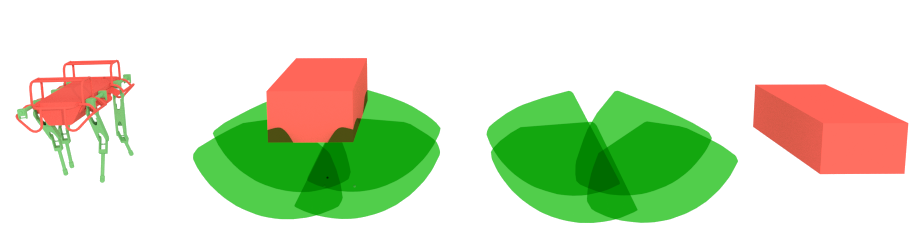
\includegraphics[width=0.95\linewidth]{figures/HyQ_roms}
%DIFDELCMD <   %%%
\DIFdelendFL \DIFaddbeginFL 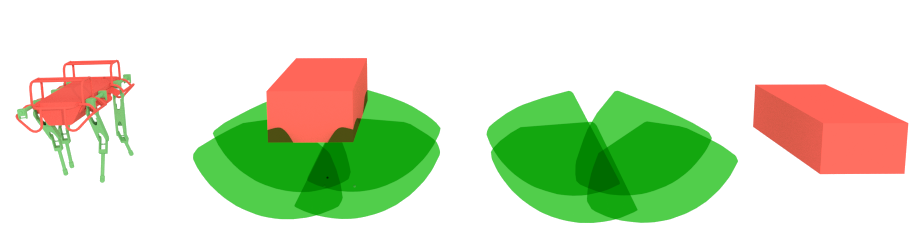
\includegraphics[width=1\linewidth]{figures/HyQ_roms}
  \DIFaddendFL \caption{
           Reachable workspace and torso bounding box of HyQ. Each green shape represent a reachable workspace $W^k$ of a limb. The red shape is $W^0$.}
		   \label{fig:HyQ_roms}
\end{figure}
% !TEX root =  ../main.tex
%~ \section{Computing a guide path in $C^0_{reach}$ ($\mathcal{P}_1$) }
\section{Root path planning in the contact reachable space}
\label{rbprm}

During the root path planning we only consider the root configuration $\mathbf{q}^0$ defined in the previous Section,
as well as the environment $O$.

Given \DIFdelbegin \DIFdel{a start and a }\DIFdelend \DIFaddbegin \DIFadd{start and }\DIFaddend goal configurations, we aim at computing a guide path $\mathbf{q}^0(t) : [0,1] \longrightarrow$ $\mathbb{R}^r$ verifying:
\begin{equation*} \label{eq:path}
\forall t \in [0,1], \mathbf{q}^0(t)  \in C_{Equil}^0
\end{equation*}
This means that any root configuration must be extended into a whole-body, static equilibrium configuration.
$C_{Equil}^0$  cannot be described analytically.

The \DIFdelbegin \DIFdel{strong }\DIFdelend \DIFaddbegin \DIFadd{main }\DIFaddend hypothesis of this work is that for a large variety of locomotion tasks, we can define a space  $C_{Reach}^0 \simeq C_{Contact}^0$, such that 
\begin{equation} \label{eq:creach}
\forall t \in [0,1], \mathbf{q}^0(t) \in C_{Reach}^0 \Rightarrow \mathbf{q}^0(t)  \in C_{Equil}^0
\end{equation}
% for \gls{cluttered} problems.
We call  $C_{Reach}^0$ the \textit{contact reachable workspace}, and detail its construction in the following.
The validity of this hypothesis is discussed in depth in Section~\ref{sec:discussion}.
%~ We describe the construction of $C_{Reach}^0$ in the following.

\subsection{Conditions for contact reachability}
The contact reachable workspace is defined as a compromise between two necessary and a sufficient condition for contact creation.

\textbf{necessary conditions:}
For a contact to be possible, an obstacle $O_i \subset O$ necessarily intersects the reachable workspace $W(\mathbf{q}^{0})$ of the robot\DIFdelbegin \DIFdel{(Figure~\ref{fig:contact_gen}--1). }\DIFdelend \DIFaddbegin \DIFadd{. %DIF >  (Figure~\ref{fig:contact_gen}--a).
 }\DIFaddend Also the torso of the robot $W^0(\mathbf{q}^{0})$ must necessarily be collision-free.
Therefore we can define an outer approximation  $ \mathcal{C}^0_{\textrm{\it Nec}} \supset$ $C_{Contact}^0$ as: 
\begin{equation}
\mathcal{C}^0_{\textrm{\it Nec}} = \{ \mathbf{q}^0 : W(\mathbf{q}^{0}) \cap O \neq \emptyset \textrm{ \textbf{and}}\ W^0(\mathbf{q}^{0}) \cap O = \emptyset \} % \\ }
 %~ & \text{ and } & A_{torso}(\mathbf{q}^{root}) \cap W = \emptyset \}
\end{equation}
%~ The inclusion $C_{Contact}^0$ $\subset \mathcal{C}^0_{\textrm{\it Nec}}$ is straightforward, but it is very important.
%~ Planning in $\mathcal{C}^0_{\textrm{\it Nec}}$ allows a strong reduction of the search space, while not discarding 
%~ any root configuration that could lead to a solution.

%~ The condition defining $\mathcal{C}^0_{\textrm{\it Nec}}$ is only necessary. This means that it might not be possible to extend a guide path planned 
%~ in $\mathcal{C}^0_{\textrm{\it Nec}}$ into a sequence of contact configurations.

\textbf{sufficient condition:}
Similarly we can define an inner approximation \mbox{$\mathcal{C}^0_{\textrm{\it Suf}} \subset $ $C_{Contact}^0$} by considering a bounding volume $B^{\textrm{\it Suf}}$ encompassing the whole robot in a given pose, except for the effector surfaces. 
\begin{equation}
\mathcal{C}^0_{\textrm{\it Suf}} = \{ \mathbf{q}^0 : W(\mathbf{q}^{0}) \cap O \neq \emptyset \textrm{ \textbf{and}}\ B^{\textrm{\it Suf}}(\mathbf{q}^{0}) \cap O = \emptyset \} % \\ }
 %~ & \text{ and } & A_{torso}(\mathbf{q}^{root}) \cap W = \emptyset \}
\end{equation}

%~ In general, the inclusion is strict, which means that we lose the completeness of the two-stage contact planner (i.e. the planner is not able to discover a path inside \mbox{$C_{reach} \setminus \mathcal{C}^0_{\textrm{\it Suf}}$}). However, the sufficient condition guarantees that any such path leads to a valid sequence of contacts.

\subsection{The compromising reachability condition}
\label{sec:scaling}
The ideal shape \DIFdelbegin \DIFdel{$B^*, W^0 \subset B* \subset B^{\textrm{\it Suf}}$ that defines }\DIFdelend \DIFaddbegin \DIFadd{$B^*, W^0 \subset B^* \subset B^{\textrm{\it Suf}}$ would define }\DIFaddend a necessary \textbf{and} sufficient condition for contact creation\DIFaddbegin \DIFadd{. 
It would guarantee that any root configuration $\mathbf{q}^{0} \in B^*$ would result in a contact configuration, while any $\mathbf{q}^{0} \notin B^*$ could not.
To our knowledge  $B^*$ }\DIFaddend has no explicit definition.
Therefore, we approximate $B^*$ to define the contact reachable space $C_{Reach}^0$.

%~ However, using a shape between $W^0$ and $B^{\textrm{\it Suf}}$ leads to a trade-off between a necessary and a sufficient condition. 
We define $W^0_s$ as the volume $W^0$ subject to a scaling transformation by a factor $s \in \mathbb{R}^+$.
%
We then consider the spaces $C_{s}^0$
 \begin{equation}
 \label{eq:reachc}
C^0_s = \{ \mathbf{q}^0 : W(\mathbf{q}^{0}) \cap O \neq \emptyset \textrm{ \textbf{and}}\ W^0_s(\mathbf{q}^{0}) \cap O = \emptyset \} % \\ }
 %~ & \text{ and } & A_{torso}(\mathbf{q}^{root}) \cap W = \emptyset \}
\end{equation}
%
The parametrization of $s$ defines a trade-off:
If $s=1$, then $W^0_s$ = $W^0$, such that $C_1^0$ = $\mathcal{C}^0_{\textrm{\it Nec}}$.
 %~ We thus consider that $s \geq 1$, since smaller values would only worsen the approximation.
By increasing $s$, the condition can become sufficient, but less and less necessary.  
Eq.~\ref{eq:reachc} thus defines the \textit{reachability condition}. We fix a value $s^*$ for $s$ and define  $C_{Reach}^0 = C^0_{s^*}$.
The computation of $s^*$ is detailed in Section~\ref{sec:params}. 
In Appendix~\ref{app:rom}, we give a generic method to compute the $W$ volumes appearing in the definition of $C_{Reach}^0$.

\subsection{Computing the guide path in $C_{reach}^0$}
$C_{Reach}^0$ can be sampled efficiently thanks to Eq.~\ref{eq:reachc}, and can thus be used with \DIFdelbegin \DIFdel{a }\DIFdelend \DIFaddbegin \DIFadd{any }\DIFaddend standard motion planner.
\DIFdelbegin \DIFdel{The only significant change is to replace the collision checking with the \textit{reachability condition}.
}\DIFdelend %DIF > ~ The only significant change is to replace the collision checking with the \textit{reachability condition}.
Our current implementation \DIFdelbegin \DIFdel{of these modifications is based on }\DIFdelend \DIFaddbegin \DIFadd{uses }\DIFaddend the Bi-RRT planner \citep{770022} provided by the HPP software~\citep{7759083}.
\DIFaddbegin \DIFadd{Our implementation is exactly the same as the pseudo-code of the original planner (which does not detail the configuration validation method). With respect to a ``classic'' implementation, the only difference is that instead of validating a configuration using collision detection, we validate it with the \textit{reachability condition}.}\DIFaddend \\

%~ \delst{However, to improve the sampling efficiency 
%~ we bias the sampling process to generate near-obstacle configurations, similarly to cite{Amato98choosinggood}.}

This Section has presented a guide path planner for the geometric root of a robot, implemented as a low-dimensional sampling-based 
algorithm. Given start and goal configurations, it outputs a continuous path for the robot's root. 
%~ \deladp{Thanks to the \textit{reachability condition}, we assume that for any configuration in the path there exists a joint configuration that results in static equilibrium.}
%~ Thanks to these modifications, the problem of planning a \gls{contact reachable} path is reduced to a geometric collision-checking problem, of low dimension (6 for HyQ, 8 for HRP-2 that has 2 joints in the torso).
%~ By doing this we can solve the problem with a sampling-based approach, in \gls{interactive} computation times.
% !TEX root =  ../main.tex
\section{From a guide path to a discrete sequence of contact configurations ($\mathcal{P}_2$)}
\label{sec:contact}
In the second phase, we compute a discrete sequence of static equilibrium configurations $\mathbf{Q}^{\overline{0}}$ given a root path
$\mathbf{q}^0(t) : [0,1] \longrightarrow$ \gls{$C_{Reach}^0$}. This contact planner uses a contact generator, used to generate static equilibrium configurations. We first describe the contact planning algorithm, before describing
the contact generator.
%~ Our planner computes guide paths in $C_{Reach}^0$ , an approximation of \gls{$C_{Equil}^0$}.
%~ As an input of this stage, we however assume an \gls{equilibrium feasible} root guide path $\mathbf{q}^0(t) : [0,1] \longrightarrow$ \gls{$C_{Equil}^0$}.
%~ If this is not the case, our planner will fail rapidly, thus allowing replanning, as discussed in Section~\ref{sec:perf}.
%~ We now consider the second problem of computing a discrete sequence of equilibrium configurations $\mathbf{Q}^{\overline{0}}$ along $\mathbf{q}^0(t)$.


%~ In this Section we first describe a single contact-generation process, that is how to generate a contact configuration for a limb, given a
%~ root location.
%~ Then, we propose an iterative algorithm to generate a discrete sequence of contact configurations in static equilibrium.

%~ Our criterion to assert efficiently the static equilibrium of the system
%~ is described in Appendix~\ref{sec:heuristics}.

\subsection{Definition of a contact sequence}
In previous contributions~\citep{DBLP:conf/iser/EscandeKMG08}, a contact plan is defined as a sequence of quasi-static equilibrium configurations
for each contact phase. For instance, a walk cycle would be described by three key configurations: a double-support configuration, a single-support configuration (a contact is broken), and another double-support configuration (a contact is created). 
Our definition of contact plan differs: between two consecutive configurations we allow both a contact break and a contact creation---if they are on the same effector. 
In the previous example, our contact plan would simply consist of the two double-support configurations. 
%However, if the contact broken and the contact created sequentially are not on the same effector, our planner outputs two distinct states.
This representation is sufficient to describe all the contact phases\DIFaddbegin \DIFadd{, because the single support phase is implicitely described}\DIFaddend . Furthermore it removes the need to \DIFdelbegin \DIFdel{have }\DIFdelend \DIFaddbegin \DIFadd{compute a }\DIFaddend single-support quasi-static \DIFdelbegin \DIFdel{configurations }\DIFdelend \DIFaddbegin \DIFadd{configuration }\DIFaddend as in the example. \DIFdelbegin \DIFdel{As }\DIFdelend \DIFaddbegin \DIFadd{Indeed, there might be a case where no quasi-static solution exists for the single support phase (because of the environment), but
there exists a dynamic motion connecting the two double support states. Such motion will be computed by our framework, because the quasi-static constraint is only required at the contact planning phase; as }\DIFaddend shown in the companion video, \DIFdelbegin \DIFdel{this allows our framework }\DIFdelend \DIFaddbegin \DIFadd{and explained in Appendix~\ref{app:optim}, our framework is able }\DIFaddend to produce dynamic motions.

\subsection{Contact planning algorithm}
Starting from an initial whole-body configuration, we compute a sequence
of whole-body configurations  $\mathbf{Q}^{\overline{0}}$ along the root path $\mathbf{q}^0(t)$.
\DIFdelbegin \DIFdel{The algorithm can be found in Appendix~\ref{app:contact}. Here we provide }\DIFdelend \DIFaddbegin \DIFadd{We first give }\DIFaddend an intuition of \DIFdelbegin \DIFdel{it.
}%DIFDELCMD < 

%DIFDELCMD < %%%
\DIFdelend \DIFaddbegin \DIFadd{the algorithm, before providing its complete pseudo-code.
%DIF > ~ The algorithm can be found in Appendix~\ref{app:contact}. Here we provide an intuition of it.
}\subsubsection{\DIFadd{Algorithm overview}}
\DIFaddend First, the root path $\mathbf{q}^0(t)$ is discretized into a sequence of $j$ key configurations:  
\begin{equation*}
	\mathbf{Q}^0 = [\mathbf{q}^0_{0}; \mathbf{q}^0_{i}; ..., \mathbf{q}^0_{j-1}]
\end{equation*} 
\DIFaddbegin 

\DIFaddend where $\mathbf{q}^0_{0}$ and $\mathbf{q}^0_{j-1}$ are the start and goal configurations. %To ensure continuity in the contact transition phases,
\DIFaddbegin \DIFadd{$j$ depends on a user-defined variable, called the discretization step. It corresponds to the ratio between the length of the path $\mathbf{q}^0(t)$}\footnote{\DIFadd{The length of the path is computed as the weighted 6D Euclidian distance
travelled along the it, with a weight of $0.7$ for the translation part, and $0.3$ for the orientation part.}}\DIFadd{, and the number
of configurations selected along it to create the contact configurations. 
}\DIFaddend Each root configuration of $\mathbf{Q}^0$ is then extended into a whole-body configuration such that:
\begin{itemize} 
\item At most one contact is not maintained (\textit{broken}) between two consecutive configurations.
\item At most one contact is added between two consecutive configurations.
\item Each configuration is in static equilibrium.
\item Each configuration is collision-free.
\end{itemize} 


%~ We want to extend the configurations of $\mathbf{Q}^0$ in such a way that continuity is preserved regarding the contact transitions.
%~ To do so, we define an algorithm that, given the current root configuration, and the previous full body configuration, computes a full body configuration 
%~ in $C_{Equil}$ such that contacts are maintained if possible.
%~ The first full body configuration of the sequence is given by the initial state of the robot.

 %~ we propose a recursive mapping $\pi$, for any $0<i<j$:
%~ \begin{equation*}
    %~ \pi\colon\left\{
    %~ \begin{aligned}		
        %~ \mathbf{Q}^0 \in C_{Equil}^0 & \longrightarrow C_{Equil} \\
        %~ %\mathbf{q}^{0}_0 &  \longrightarrow  \mathbf{q}_{start} \\
        %~ \mathbf{q}^{0}_i &  \longrightarrow  g(\mathbf{q}_{i - 1},\mathbf{q}^{0}_i) 
    %~ \end{aligned}
    %~ \right.
%~ \end{equation*} 
%~ $g$ is the method that extends a root configuration into a full-body configuration. At each step, it tries to generate a contact configuration that preserves as much as possible
%~ the previous contacts while allowing for static equilibrium. The objective is thus to characterize $g$.
%~ We initialize the recurrence with $\pi(\mathbf{q}^0_{0}) = \mathbf{q}_0$ the initial configuration of the robot.

%~ The function $g$ is defined independently by $g^k$ for each limb $R^k$. In defining $g^k$, two aspects must be considered. Is the limb $R^k$ in contact? And which criteria is it optimizing? 

\DIFdelbegin \subsubsection{\DIFdel{Maintaining a contact in the sequence}}
%DIFAUXCMD
\addtocounter{subsubsection}{-1}%DIFAUXCMD
\DIFdelend \DIFaddbegin \paragraph{\DIFadd{Maintaining a contact in the sequence}}
\DIFaddend 

%~ Figure~\ref{fig:break_contact} illustrates the contact-persistence strategy.
If kinematically possible, a limb in contact at step $i-1$ remains in contact at step $i$ (Figure~\ref{fig:break_contact}). 
%~ The contact is broken if an inverse-kinematics solver fails to find a collision-free limb configuration that satisfies joint limits. 
%~ The solver is directly provided by the HPP software.
Otherwise the contact is broken and a collision-free configuration is assigned to the limb.
If two or more contacts can't be maintained between two consecutive configurations, one or more intermediate configurations are added, to ensure
that at most one contact is broken between two sequential configurations.
%~ For these steps the root configuration is the same as for the previous step, with the difference that
%~ one faulty contact is repositioned, in the hope that it will not be broken at the next step.

\begin{figure}[t]
\centering
  \DIFdelbeginFL %DIFDELCMD < \begin{overpic}[width=0.9\linewidth]{figures/break_contact}
%DIFDELCMD < 		%%%
\DIFdelendFL \DIFaddbeginFL \begin{overpic}[width=1\linewidth]{figures/break_contact}
		\DIFaddendFL \put (0,4) {1} 
		\put (25,4) {2} 
		\put (50,4) {3} 
		\put (76,4) {4} 
		%~ \put (68,58) {3.a)} 
		%~ \put (5,27) {3.b)} 
		%~ \put (37,27) {4.a)} 
		%~ \put (68,27) {4.b)} 
	\end{overpic}
\caption{Contacts are maintained if joint limits and collisions constraints are respected (2). They are broken otherwise(3,4). The green line represents the root path. \DIFaddbeginFL \DIFaddFL{The blurred character
represents the previous contact configuration.}\DIFaddendFL }
		   \label{fig:break_contact}
\end{figure}

%~ \begin{figure}[t]
%~ \centering
  %~ \begin{overpic}[width=0.6\linewidth]{figures/generate_contact}
		%~ \put (5,58) {1)} 
		%~ \put (37,58) {2)} 
		%~ \put (68,58) {3.a)} 
		%~ \put (5,27) {3.b)} 
		%~ \put (37,27) {4.a)} 
		%~ \put (68,27) {4.b)} 
	%~ \end{overpic}
%~ \caption{Contacts are generated when the configuration is not balanced.}
		   %~ \label{fig:generate_contact}
%~ \end{figure}


%\subsection{Generation of a contact configuration}  
\DIFdelbegin \subsubsection{\DIFdel{Creating contacts}}
%DIFAUXCMD
\addtocounter{subsubsection}{-1}%DIFAUXCMD
\DIFdelend \DIFaddbegin \paragraph{\DIFadd{Creating contacts}}
\DIFaddend Contacts are created using a FIFO approach: we try first to create a contact with the limb that has been contact-free the longest. If the contact creation does not succeeds, the limb is pushed on top of the queue, and will only be tried again after the others. \DIFaddbegin \\ \\
\DIFaddend %~ \begin{enumerate}
%~ \item \deladp{At most one contact creation happens between two consecutive steps. }
%~ \item \deladp{A contact is validated if and only if the resulting configuration is in static equilibrium;}
%~ \item \deladp{We use a FIFO approach:  we always try first to create a contact with the limb that has been contact-free the longest. If the contact creation
%~ was not successful for a limb, the limb is pushed on top of the queue, and will only be tried again after the others.}
%~ \end{enumerate}

%~ \deladp{However, in practice the planner is successful in the large majority of cases, as discussed in Section~\ref{sec:perf}.}


%DIF >  !TEX root =  ../main_tro.tex
\DIFaddbegin \subsubsection{\DIFadd{Pseudo-code of the Algorithm}}
\label{app:contact}


\DIFadd{First, we define an abstract structure State,
that describes a contact configuration.
The use of queues allows a FIFO approach regarding the order 
in which contacts are tested: we try to replace older contacts first when necessary.
Thus the algorithm is deterministic even though it can handle acyclic motions. }\\

\begin{lstlisting}]
Struct Limb
{
    // Limb Configuration
    Configuration qk;
    // Effector position in
    // world coordinates
    vector6 pk;
};

Struct State
{
    // root location
    Configuration q0;
    // List of limbs not in contact
    queue<Limb> freeLimbs;
    // List of limbs in contact
    queue<Limb> contactLimbs;
};
\end{lstlisting}

\DIFadd{From the start configuration, given as an input by the user,
we create the initial state $s0$.
Algorithm~\ref{alg:interpolate}  is then called with $s0$, as well as the discretized path 
$\mathbf{Q}^0$, as input parameters.
}

\begin{algorithm}[!tbp]
\caption{\DIFadd{Discretization of a path}} \label{interpolate}
	\begin{algorithmic}[1]
	%DIF > ~ \Function{GenerateConfiguration}{}
	\Function{Interpolate}{$s0$,$\mathbf{Q}^0$, $MAX\_TRIES$}
		\State \DIFadd{$list<$State$>$ $states = [s0]$
		}\State \DIFadd{$nb\_fail = 0$ 
		}\State \DIFadd{$i = 1;$ /*Current index in the list*/
		}\While {\DIFadd{$i < length(\mathbf{Q}^0)$}}
			\State \DIFadd{State $pState = last\_element(states)$
			}\State \DIFadd{State $s =$ \textsc{GenFullBody}$(pState, \mathbf{Q}^0[i])$
			}\If {\DIFadd{$s != NULL $}}
				\State \DIFadd{$nb\_fail = 0$
				}\State \DIFadd{$i += 1$
				}\State \DIFadd{\textbf{return} $\mathbf{q}^{0}$
			}\Else
				\State \DIFadd{$nb\_fail += 1$
				}\If {\DIFadd{$nb\_fail == MAX\_TRIES$}}
					\State \DIFadd{\textbf{return} $FAILURE$
				}\EndIf				
				\State \DIFadd{$s = $\textsc{IntermediateContactState}$(pState)$
			}\EndIf
			\State \DIFadd{$push\_back(states, s)$
		}\EndWhile
		\State \DIFadd{\textbf{return} $states$
	}\EndFunction
\end{algorithmic}
\label{alg:interpolate}
\end{algorithm}

\DIFadd{At each step, \textsc{GenFullBody} is called with the previous state as a parameter, as well
as a new root configuration. \textsc{GenFullBody} returns a new contact configuration, if it succeeded
in computing a configuration with only one contact switch occurring.
Otherwise, the method \textsc{IntermediateContactState} is called.
It repositions one end effector (either a free limb, or the oldest active contact) towards a new contact position if possible.
This repositioning allows to increase the odds that the contact can be maintained at the next step.
Algorithm~\ref{alg:pi} gives the pseudo code for \textsc{GenFullBody}.
}

\begin{algorithm}[!tbp]
\caption{\DIFadd{Full body contact generation method}} \label{interpolate}
	\begin{algorithmic}[1]
	%DIF > ~ \Function{GenerateConfiguration}{}
	\Function{\textsc{GenFullBody}}{$pState$,$\mathbf{q}^0$}
		\State \DIFadd{State $newState$
		}\State \DIFadd{$newState.q0 = \mathbf{q}^0$
		}\State \DIFadd{$newState.freeLimbs = pState.freeLimbs$
		}\State \DIFadd{/*First try to maintain previous contacts*/
		}\State \DIFadd{$nbContactsBroken = 0$
		}\For {\DIFadd{\textbf{each} Limb $k$ in $pState.contactLimbs$}}
			\If {\DIFadd{$!$\textsc{MaintainContact}$(pState,\mathbf{q}^0,k)$}}
				\State \DIFadd{$nbContactsBroken += 1$
				}\If {\DIFadd{$nbContactsBroken > 1$}}				
					\State \DIFadd{\textbf{return} $NULL$
				}\EndIf				
				\State \DIFadd{$push(newState.freeLimbs,k)$
			}\Else 					
				\State \DIFadd{$push(newState.contactLimbs,k)$
			}\EndIf
		\EndFor
		\For {\DIFadd{\textbf{each} Limb $k$ in $pState.freeLimbs$}}
			\If {\DIFadd{\textsc{GenerateContact}$(\mathbf{q}^0,k)$}}	
				\State \DIFadd{$push(newState.contactLimbs,k)$
				}\State \DIFadd{$remove(newState.freeLimbs,k)$		
				}\State \DIFadd{\textbf{return} $newState$
			}\EndIf
		\EndFor
		\If {\DIFadd{\textsc{IsInStaticEquilibrium}$(newState)$}}
			\State \DIFadd{\textbf{return} $newState$
		}\Else
			\State \DIFadd{\textbf{return} $NULL$
		}\EndIf
	\EndFunction
\end{algorithmic}
\label{alg:pi}
\end{algorithm}

\DIFadd{The method \textsc{MaintainContact}$(pState,\mathbf{q}^0,k)$ performs inverse kinematics to reach the previous contact position for the Limb.
If it succeeds, the new limb configuration is assigned to $k$. If it fails, a random collision free configuration is assigned to $k$.
}

\DIFadd{The method \textsc{IsInStaticEquilibrium} returns whether a given state is in static equilibrium.
}

\DIFadd{The pseudo code for the method \textsc{IntermediateContactState} is given by Algorithm~\ref{alg:repo}.
}


\DIFadd{\textsc{GenerateContact}$(\mathbf{q}^0,k)$ is a call to the contact generator presented in the following Section~\ref{sec:single_contact}.
 It generates a contact configuration in static equilibrium, and assigns the corresponding configuration to $k$.
If it fails, $k$ remains unchanged if it is collision free, otherwise it is assigned a random collision free configuration.
}



\begin{algorithm}[!tbp]
\caption{\DIFadd{Adds or repositions a contact for one limb}} \label{interpolate}
	\begin{algorithmic}[1]
	\Function{IntermediateContactState}{$state$}
		\State \DIFadd{$i=0$
		}\While {\DIFadd{$i<length(states.freeLimbs)$}}
			\State \DIFadd{Limb $k = pop(states.freeLimbs)$
			}\If {\DIFadd{\textsc{GenerateContact}$(state.q0,k)$}}	
				\State \DIFadd{$push(newState.contactLimbs,k)$			
				}\State \DIFadd{\textbf{return}
			}\Else
				\State \DIFadd{$i+=1$
				}\State \DIFadd{$push(states.freeLimbs,k)$		
			}\EndIf
		\EndWhile
		\State \DIFadd{$i=0$
		}\While {\DIFadd{$i<length(states.contactLimbs)$}}
			\State \DIFadd{Limb $k = pop(states.contactLimbs)$
			}\State \DIFadd{Limb $copy = k$
			}\State \DIFadd{$i+=1$
			}\If {\DIFadd{\textsc{GenerateContact}$(state.q0,k)$}}	
				\State \DIFadd{$push(newState.contactLimbs,k)$			
				}\State \DIFadd{\textbf{return}
			}\Else
				\State \DIFadd{$push(newState.contactLimbs,copy)$	
			}\EndIf
		\EndWhile
		\DIFadd{/*Fails if impossible to relocate any effector*/
		}\State \DIFadd{\textbf{return} $FAILURE$
	}\EndFunction
\end{algorithmic}
\label{alg:repo}
\end{algorithm}

%DIF > ~ \section{Derivation of the manipulability ellipsoid}
%DIF > ~ \label{app:manipulability}
%DIF > ~ 
%DIF > ~ Again, we assume that $\mathbf{J}$ is full rank. We discard the $k$ indices, and write the pseudo-inverse of $\mathbf{J}$ as $\mathbf{J}^{\dagger}$.
%DIF > ~ \begin{eqnarray*}
%DIF > ~ \mathbf{\dot{p}} & =  & \mathbf{J} \dot{\mathbf{q}} \\ 
%DIF > ~ \mathbf{\dot{q}} & =  & \mathbf{J}^{\dagger} \dot{\mathbf{p}} \\ 
%DIF > ~ \mathbf{\dot{q}}^T & =  & \dot{\mathbf{p}}^T \mathbf{J}^{\dagger T} \\ 
%DIF > ~ \mathbf{\dot{q}}^T\mathbf{\dot{q}} & =  & \dot{\mathbf{p}}^T \mathbf{J}^{\dagger T} \mathbf{J}^{\dagger} \dot{\mathbf{p}}\\ 
%DIF > ~ \end{eqnarray*}
%DIF > ~ 
%DIF > ~ Then, the equality $\mathbf{J}^{\dagger T} \mathbf{J}^{\dagger} = (\mathbf{J}\mathbf{J}^T)^{-1}$ follows from the SVD decomposition of each term
%DIF > ~ ~\citep{ben2003generalized}.

\DIFaddend \subsection{Contact generator}
\label{sec:single_contact}

\begin{figure*}
  \centering
  \begin{overpic}[width=0.8\linewidth]{figures/contact_gen}
		\put (1,1) {a} 
		\put (22,1) {b} 
		\put (42,1) {c} 
		\put (62,1) {d} 
		\put (83,1) {e} 
	\end{overpic}
  \caption{Generation of a contact configuration for the right leg of HRP-2. (a): Selection of reachable obstacles. (b): Entries of the limb samples database (with $N = 4$). (c): With a proximity query between the octree database and the obstacles, configurations too far from obstacles are discarded. (d): The best candidate according to a user-defined heuristic $h$ is chosen. (e): The final contact is achieved using inverse kinematics.}
  \label{fig:contact_gen}
\end{figure*}

Given a configuration of the root and the list of effectors that should be in contact, the contact generator computes the configuration of the limbs such that contacts are properly satisfied and the robot is in static equilibrium:

\begin{equation}
\label{eq:contact_gen}
	\mathbf{q}^{\overline{k}}  \longrightarrow \mathbf{q}^k, (\mathbf{q}^{k} \oplus \mathbf{q}^{\overline{k}}) \in  C_{Equil} \textrm{ \textbf{and}}\ \mathbf{q}^k \in  C_{Contact}^k 
\end{equation}

In previous works~\cite{DBLP:conf/iser/EscandeKMG08,Bouyarmane2009}, the generation of contact is typically implemented by randomly sampling configurations and projecting the whole robot configuration onto the closest surfaces with an inverse kinematics solver.
In case of failure of the projection, the process would randomly iterate.


We propose two modifications of this general algorithm principle.
First our contact generator handles each limb $R^k$ independently.
By handling each limb separately, we reduce the complexity of the generation of contact configurations.
This is made possible thanks to the reachability condition in $\mathcal{P}_1$ that produces a root path that we can afford not to modify in $\mathcal{P}_2$, and because we allow both a contact break and a contact creation between two consecutive configurations of the contact sequence.
Second, we rely on off-line generation of configuration candidates.
%~ Contact generation is typically addressed by randomly sampling a limb configuration, before projecting the effector onto the closest surface with an inverse kinematics solver.
%~ This process is repeated until either a solution for Eq.~(\ref{eq:contact_gen}) is found, or the generator fails, according to a user-defined maximum number of trials.
%~ We favor a modified implementation of this naive approach, more computationally efficient, introduced in our previous work~\citep{Tonneau2014}.



%~ Given a configuration $\mathbf{q}^{\overline{k}}$ of the root and all the limbs but $R^k$, we look for a limb configuration $\mathbf{q}^k$ such that
%~ $R^k$ is in contact, and not colliding (neither with parts of the robot nor with the environment).
%~ While exhibiting analytically a $\mathbf{q}^{k}$ does not seem tractable, we can iteratively try to generate one as follows:
%~ \begin{enumerate}
%~ \item Generate randomly a collision-free limb configuration;
%~ \item Project the end-effector onto the closest surface with inverse kinematics;
%~ \item If a valid solution is found, stop. Otherwise repeat from step 1.
%~ \end{enumerate}


%~ We favor a modified implementation of this naive approach, more computationally efficient, introduced in our previous work~\citep{Tonneau2014}.

We define $C_{Contact}^{\epsilon} \supset C_{Contact}$ as the set of configurations such that the minimum \DIFaddbegin \DIFadd{3D }\DIFaddend distance 
between an effector and an obstacle is less than $\epsilon \in \mathbb{R}$.
We then apply the following steps:
\begin{enumerate}
\item Generate off-line $N$ valid sample limb configurations $\mathbf{q}^k_i,  0 \leq i < N$ (We choose $N=10^4$);
\item Using the end-effector positions $\mathbf{p}(\mathbf{q}^k_i)$ as indices, store each sample in an octree data structure;
\item At runtime, when contact creation is required, intersect the octree and the environment\DIFaddbegin \footnote{\DIFadd{this operation is achieved natively by the fcl library https://flexible-collision-library.github.io/}} \DIFaddend to retrieve the list of samples $S \subset C_{Contact}^{\epsilon}$ close to contact (Figure~\ref{fig:contact_gen} (b) and (c));
\item Use a user-defined heuristic $h$ to sort $S$;
\item If $S$ is empty, stop (failure). Else select the first configuration of $S$. Project it onto contact using inverse kinematics. (Figure~\ref{fig:contact_gen} (d) and (e));
\item If Eq.~\ref{eq:contact_gen} is verified, stop (success). Otherwise remove the element from $S$ and go to step 5.
\end{enumerate}

%DIF < ~ This approach has two main advantages.
%DIF < ~ First, this allows us to select a large number of candidates in a single proximity request.
%DIF < ~ Having several candidates is interesting, because it allows to compare them using a user-selected heuristic $h$, thus obtaining
%DIF < ~ a locally-optimal candidate.
%DIF < ~ Furthermore, the fact that the candidates are already close to contact increases the odds that the inverse kinematics will converge to a valid solution in a small number of iterations.
%DIF < ~ Regarding convergence, it is immediate to verify that as $N$ grows, the probability of finding a solution if it exists converges to 1.
%DIF < ~ $N$ is a parameter that allows us to specify the trade-off between exhaustiveness and efficiency.
\DIFdelbegin \DIFdel{The reader is referred to our previous work for an extensive discussion on the benefits of this approach, and the optimal choice 
of the parameter $N$~\citep{Tonneau2014}.
Our criterion to assert efficiently the static equilibrium of the robot, as well as the heuristics $h$ are detailed inAppendix~\ref{sec:heuristics}.
}\DIFdelend %DIF > ~ The reader is referred to our previous work for an extensive discussion on the benefits of this approach, and the optimal choice 
%DIF > ~ of the parameter $N$~\citep{Tonneau2014}. Our criterion to assert efficiently the static equilibrium of the robot, as well as the heuristics $h$ are detailed in Appendix~\ref{sec:heuristics}.
\DIFaddbegin \DIFadd{Because the distance $\epsilon$ does not account for the variation in orientation, several samples of $ C_{Contact}^{\epsilon}$  may turn out to be unfeasible at the time of projection. One could consider additionally filtering $ C_{Contact}^{\epsilon}$ based on the orientation with respect to the obstacle normal, but in our experience we did not notice
any significant improvement in the computational performances of the planner, so we do not perform this additional step. 
 }\DIFaddend 

%DIF < ~ It should be noted that a failure case for our contact generator does not necessarily mean that the planner will globally fail. Indeed,
%DIF < ~ for a given root configuration, if contact configurations are found for other limbs, resulting in static equilibrium, the configuration will be accepted despite
%DIF < ~ the failure to generate a contact.
\DIFaddbegin \DIFadd{In all our experiments, the heuristic $h$ is implemented as a variation of a manipulability-based heuristic~\cite{Yoshikawa1984}. The manipulability is a real number that quantifies how 
``good'' a configuration is to perform a given task, based on the analysis of the Jacobian matrix. With such heuristics, a configuration can be chosen because it is far from singularities, and thus allows mobility in all directions. On the contrary, it can be chosen because it is particularly efficient to exert a force in a desired direction. In our experiments, the former solution is usually chosen for computing leg contacts, while the latter is used for computing hand contacts. We recall the manipulability measure and its derivatives in Appendix~\ref{sec:heuristics}.
}\DIFaddend 

%DIF < ~ In this Section, we have thus defined a deterministic contact planning algorithm.
%DIF < ~ The determinism of this algorithm makes it efficient, at the cost of not being probabilistically complete.
\DIFaddbegin \DIFadd{Finally, to verify that a configuration is in static equilibrium, we use a new robust LP formulation. It replaces the computationally inefficient double description
approach used in our previous work~\cite{tonneauisrr15}, and presented in the following Section~\ref{sec:Equil}.
}



%DIF > ~ TODO: $h$ in appendix, the static equilibrium is here ~\ref{sec:Equil}

\DIFaddend % !TEX root =  ../main.tex
\DIFaddbegin 

\section{\DIFadd{A criterion for robust static equilibrium}}
\label{sec:Equil}
%DIF > ~ The planner is designed so that any generated contact configuration is in static equilibrium.
%DIF > ~ We are interested in a robust 
%DIF > ~ criterion, that ensures that the robot remains in equilibrium in a real-world application, regardless of perception and control uncertainties.

\DIFadd{We first give a linear program (LP) that verifies whether a contact configuration allows for static equilibrium. This LP is the same that was proposed in  \citep{Prete2016}.
From this formulation we derive a new LP that quantifies the robustness of the equilibrium to uncertainties in the contact forces.
In turn, from this value we can either choose the most robust candidate, or set a threshold on the required robustness. 
%DIF > ~ While the presented LP is original, it is based on an analysis of the problem that we proposed in, where the interested reader can find more details.
}


\subsubsection{\DIFadd{Conditions for static equilibrium}}
\DIFadd{We first define the variables of the problem, for $e$ contact points, expressed in world coordinates:
}\begin{itemize}
\item \DIFadd{$\mathbf{c} \in \mathbb{R}^3$ is the robot center of mass (COM);
}\item \DIFadd{$m \in \mathbb{R}$ is the robot mass;
}\item \DIFadd{$\mathbf{g} = [0,0,-9.81]^T$ is the gravity acceleration;
}\item \DIFadd{$\mu$ is the friction coefficient;
}\item \DIFadd{for the i-th contact point $1 \leq i \leq e$:
	}\begin{itemize}
	\item \DIFadd{$\mathbf{p_i}$ is the contact position;
	}\item \DIFadd{$\mathbf{f_i}$ is the force applied at $\mathbf{p_i}$;
	}\item \DIFadd{$\mathbf{n}_i,\mathbf{\boldsymbol\upgamma}_{i1},\mathbf{\boldsymbol\upgamma}_{i2}$ form a local Cartesian coordinate system centered at $\mathbf{p_i}$. $\mathbf{n}_i$ is aligned
	with the contact surface normal, and the $\mathbf{\boldsymbol\upgamma}_i$s are tangent vectors.
	}\end{itemize}
\end{itemize}

\DIFadd{According to Coulomb's law, the non-slipping condition is verified if all the contact forces lie in the friction cone defined by the surface.
As classically done, we linearize the friction cone in a conservative fashion with a pyramid included in it, described by four generating rays of unit length. We choose for instance:
}\begin{equation*}
\DIFadd{\mathbf{V}_{i} = \mat{\mathbf{n}_{i} + \mu \mathbf{\boldsymbol\upgamma}_{i1} & \mathbf{n}_{i} -\mu \mathbf{\boldsymbol\upgamma}_{i1} & \mathbf{n}_{i} + \mu \mathbf{\boldsymbol\upgamma}_{i2} & \mathbf{n}_{i} - \mu \mathbf{\boldsymbol\upgamma}_{i2}}^T
}\end{equation*}

\DIFadd{Any force belonging to the linearized cone
can thus be expressed as a positive combination of its four generating rays.
}

\begin{equation*}
\DIFadd{\forall i  \qquad  \exists \bm{\beta}_i \in \mathbb{R}^{4} : \bm{\beta}_i \ge 0 \text{ and } \mathbf{f}_{i} = \mathbf{V}_{i} \bm{\beta}_i,
}\end{equation*}
\DIFadd{where $\bm{\beta}_i$ contains the coefficients of the cone generators.
We can then stack all the constraints to obtain:
}\begin{equation}\DIFadd{\label{eq:gen}
\exists \bm{\beta} \in \mathbb{R}^{4e} ,  \bm{\beta} \ge 0 \text{ and } \mathbf{f} = \mathbf{V} \bm{\beta},
}\end{equation}
\DIFadd{where $\mathbf{V} = \diag{ \{\mathbf{V}_1, \dots, \mathbf{V}_e\} }$, and $\mathbf{f} = (\mathbf{f}_0,...,\mathbf{f}_e)$.
}

\DIFadd{From the Newton-Euler equations, to be in static equilibrium the contact forces have to compensate the gravitational forces:
}


\begin{align} \DIFadd{\label{eq:new_eul}
\underbrace{
\mat{\mathbf{I}_3 & \dots & \mathbf{I}_3 \\
\hat{\mathbf{p}}_1 & \dots & \hat{\mathbf{p}}_e} \mathbf{V}
}_\mathbf{G} \bm{\beta}, = 
\underbrace{\mat{\mathbf{0}_{3\times 3} \\ m \hat{\mathbf{g}}}}_{\mathbf{D}} \mathbf{c} + 
\underbrace{\mat{-m\mathbf{g} \\ \mathbf{0}}}_{\mathbf{d}}
}\end{align}
\DIFadd{where $\hat{\mathbf{x}} \in \R{3}{3}$ is the cross-product matrix associated to $\mathbf{x}$.
}


\DIFadd{If there exists a $\bm{\beta}^*$ satisfying }\eqref{eq:gen} \DIFadd{and }\eqref{eq:new_eul}\DIFadd{, it means that the configuration is in static equilibrium.
The problem can then be formulated as an LP:
}

\begin{equation} \DIFadd{\label{eq:lin_prog} \begin{aligned}
\find \quad & \bm{\beta} \in \Rv{4e} \\
%~ \st \quad &\mathbf{G} \bm{\beta} = \mathbf{D}^{xy} \mathbf{c}^{xy} + \mathbf{d} \\
\st \quad &\mathbf{G} \bm{\beta} = \mathbf{D} \mathbf{c} + \mathbf{d} \\
& \bm{\beta} \ge 0 \\
\end{aligned} }\end{equation}

\subsubsection{\DIFadd{Formulation of a robust LP}}
\DIFadd{Let $b_0 \in \mathbb{R}$ be a scalar value. We now define the following LP:
}

\begin{equation} \DIFadd{\label{eq:lin_prog_rob} \begin{aligned}
\find \quad & \bm{\beta} \in \Rv{4e}, b_0 \in \Rv{} \\
\minimize  \quad & -b_0 \\
\st \quad &\mathbf{G} \bm{\beta} = \mathbf{D} \mathbf{c} + \mathbf{d} \\
%~ \st \quad &\mathbf{G} \bm{\beta} = \mathbf{D}^{xy} \mathbf{c}^{xy} + \mathbf{d} \\
& \bm{\beta} \ge b_0 \bm{1}\\
\end{aligned} }\end{equation}

\DIFadd{We observe that if $b_0$ is positive then }\eqref{eq:lin_prog} \DIFadd{admits a solution, and $b_0$ is proportional to the minimum distance of the contact forces to the boundaries of the friction cones.
If $b_0$ is negative, the configuration is not in static equilibrium, and $b_0$ indicates ``how far'' from equilibrium the configuration is. We thus use $b_0$ as a measure of robustness.
%DIF > ~ One advantage of $b_0$ is that it gives a constant margin 
A simple approach to robustness consists in choosing a smaller friction coefficient, to constrain the forces to lie away from the boundaries of the real cone.  However, this would result in a small safety margin for forces of low magnitude, and an excessively big safety margin for large forces as the boundaries grow more and more appart. In comparison, our margin $b_0$ is constant, and provides a helpful mean to compare the robustness of different contact configurations.
}

\DIFadd{In our implementation, rather than solving directly }\eqref{eq:lin_prog_rob}\DIFadd{, we solve an equivalent problem of smaller dimension that we get by taking the dual of }\eqref{eq:lin_prog_rob} \DIFadd{and eliminating the Lagrange multipliers associated to the inequality constraints:
}\begin{equation} \DIFadd{\label{eq:dual} \begin{aligned}
\find \quad & \bm{\nu} \in \Rv{6}\\
\maximize  \quad & -(\mathbf{D} \mathbf{c} + \mathbf{d})^T \bm{\nu} \\
\st \quad &\mathbf{G}^T \bm{\nu} \ge 0 \\
& \mathbf{1}^T \mathbf{G}^T \bm{\nu} = 1 \\
\end{aligned} }\end{equation}

\DIFadd{Indeed, from Slater's conditions \citep{Boyd:2004:CO:993483}, we know that the optimal values of an LP and its dual are equal.
Therefore the optimal value $\bm{\nu}^*$ gives the optimal value $b_0^*$ through the equality $b_0^* = (\mathbf{D} \mathbf{c} + \mathbf{d})^T \bm{\nu}^*$.
 %DIF > ~ Thus the optimal value of the LP~\eqref{eq:dual} is indeed the optimal $b_0$.
}

\section{\DIFadd{Source code of our planner}}
\label{app:hpp}
\DIFadd{Our planner is implemented using the Humanoid Path Planner (HPP) software, introduced in~\cite{7759083}.
HPP is an open source motion planning framework developed by the Gepetto team at LAAS-CNRS.
HPP implements the standard tools and algorithms used in motion planning,
such as the Bi-RRT planner from which RB-RRT is derived.
}

\DIFadd{The robot models used in our experiments are described using the standard urdf file format, compatible with HPP.
}

\DIFadd{Our implementation of the planner is also open source.
Both HPP and our planner can be simply downloaded and compiled by following the instructions on
}\url{https://humanoid-path-planner.github.io/hpp-doc/download.html?branch=rbprm}\DIFadd{. 
%DIF >  !TEX root =  ../main_tro.tex
}\DIFaddend \section{Results}
\label{sec:results}
In this section we present some of the results obtained with our planner. The complete sequences are shown in the companion video.
Specifically, we demonstrate the planner for two legged robots, in a large variety of environments: the humanoid HRP-2 and the quadruped HyQ.
\DIFdelbegin \DIFdel{Finally, a last example suggests possible applications to dexterous manipulation.
}\DIFdelend %DIF > ~ Finally, a last example suggests possible applications to dexterous manipulation.

\DIFdelbegin \DIFdel{At the end of the video, we validate our contact plans by exhibiting a }\DIFdelend \DIFaddbegin \DIFadd{Our contact plans are then interpolated with a dedicated }\DIFaddend solution to the interpolation problem $\mathcal{P}_3$. \DIFaddbegin \DIFadd{This allows us to validate the obtained
motions in a dynamic simulator. This validation is an important contribution as it increases the confidence that the contact plans we compute can effectively
result in feasible motions on the real robot. One motion is demonstrated on the real HRP-2 robot.
%DIF > ~ The obtained motions can be seen at at the end of the video.
}\DIFaddend 

At the end of this section, we discuss the role of the parameters of our framework. We then provide the \textit{interactive} computation times obtained in each case.
We also compare the times obtained with HRP-2 with respect to previous works.

\DIFdelbegin \DIFdel{These scenarios complement the ones demonstrated on virtual avatars (Figure~\ref{fig:robots_old})in our previous ISRR paper~\citep{tonneauisrr15} and video}\footnote{%DIFDELCMD < \url{http://youtu.be/LmLAHgGQJGA}%%%
}%DIFAUXCMD
\addtocounter{footnote}{-1}%DIFAUXCMD
\DIFdel{.
}\DIFdelend \DIFaddbegin \subsection{\DIFadd{Experimental validation of the contact plans}} \label{sec:valid}
%DIF > ~ \adnote{I added the description of the simulations here, but I wonder whether this part should not be moved to the beginning of the Results section.}
\DIFadd{To generate continuous movements from our contact plans we used either the framework proposed in \cite{Carpentier2016}, or our own implementation of a $\mathcal{P}_3$ solver (Appendix~\ref{app:optim}).
The resulting movements have been validated either on the real HRP-2 robot (details can be found in~\cite{Carpentier2016}), or with our dynamic simulator, based on a state-of-the-art algorithm~\cite{Kaufman2008}.
In the simulations we controlled the robot with a standard inverse-dynamics controller~\cite{DelPrete2015b}.
This controller tries to follow the given whole-body trajectories, giving higher priority to the center-of-mass and end-effectors tracking with respect to the joint tracking.
The controller also makes sure that the resulting contact forces lie inside the specified friction cones (we used a friction coefficient of 0.3), and that the joint position, velocity and torque limits are satisfied.
The companion video shows the obtained motions.
}

%DIF > ~ These scenarios complement the ones demonstrated on virtual avatars (Figure~\ref{fig:robots_old}) in our previous ISRR paper~\citep{tonneauisrr15} and video\footnote{\url{http://youtu.be/LmLAHgGQJGA}}.
\DIFaddend %~ (Figure~\ref{fig:robots_old}).
 %~ We invite the interested reader to watch the ISRR video (\url{http://youtu.be/LmLAHgGQJGA}), and 
%~ to refer to the previous paper for a discussion on these results.

%~ We say that the planning is \gls{interactive} when the computation time for one step is lesser than the
%~ time to execute it. We arbitrarily approximate this time to one second.

\DIFdelbegin %DIFDELCMD < \begin{figure}[t]
%DIFDELCMD < \centering
%DIFDELCMD <   \begin{overpic}[width=1\linewidth]{figures/robots_old}
%DIFDELCMD < 		%%%
%DIF < ~ \put (5,) {1)} 
		%DIF < ~ \put (37,) {2)} 
		%DIF < ~ \put (68,) {3.a)} 
		%DIF < ~ \put (5,27) {3.b)} 
		%DIF < ~ \put (37,27) {4.a)} 
		%DIF < ~ \put (68,27) {4.b)} 
	%DIFDELCMD < \end{overpic}
%DIFDELCMD < %%%
%DIFDELCMD < \caption{%
{%DIFAUXCMD
\DIFdelFL{Virtual avatars in various scenarios demonstrated in our conference paper.}}
		   %DIFAUXCMD
%DIFDELCMD < \label{fig:robots_old}
%DIFDELCMD < \end{figure}
%DIFDELCMD < %%%
\DIFdelend %DIF > ~ \begin{figure}[t]
%DIF > ~ \centering
  %DIF > ~ \begin{overpic}[width=1\linewidth]{figures/robots_old}
	%DIF > ~ \end{overpic}
%DIF > ~ \caption{Virtual avatars in various scenarios demonstrated in our conference paper.}
		   %DIF > ~ \label{fig:robots_old}
%DIF > ~ \end{figure}

\subsection{Description of the scenarios}
In all the scenarios considered, the formulation of the problem is always the same:
a start and goal root \DIFdelbegin \DIFdel{configurations }\DIFdelend \DIFaddbegin \DIFadd{configuration }\DIFaddend are provided as input (except in the stair climbing scenario where the start whole body configuration is given).
The framework computes the initial contact configuration, and outputs a sequence of contact configurations connecting it to the goal.
In each scenario we detail the contacts involved and the heuristics chosen (either $h_{\textrm{\it EFORT}}$, $h_{vel}$ or $h_{w}$, all of which are defined in the Appendix~\ref{sec:heuristics}).
 %~ and the constraints on the reachable workspaces (for instance in all the scenarios, the reachable workspaces of the legs of HRP-2 are always required to intersect with the environment). 
%~ The companion video presents the complete contact sequence obtained in all these scenarios.

% \subsubsection*{Truck egress (Figure~\ref{res_truck_pres} and Figure~\ref{res_truck_bd}) -- Humanoid and insectoid robots.}
%\subsubsection*{Truck egress -- Humanoid and insectoid robots (Figure~\ref{res_truck_bd}).}
\DIFdelbegin \subsubsection{\DIFdel{HRP-2 -- Steep staircase (Figure~\ref{fig:stair_robust})}}
%DIFAUXCMD
\addtocounter{subsubsection}{-1}%DIFAUXCMD
\DIFdelend 


\DIFdelbegin %DIFDELCMD < \begin{figure}
%DIFDELCMD <   \centering
%DIFDELCMD <   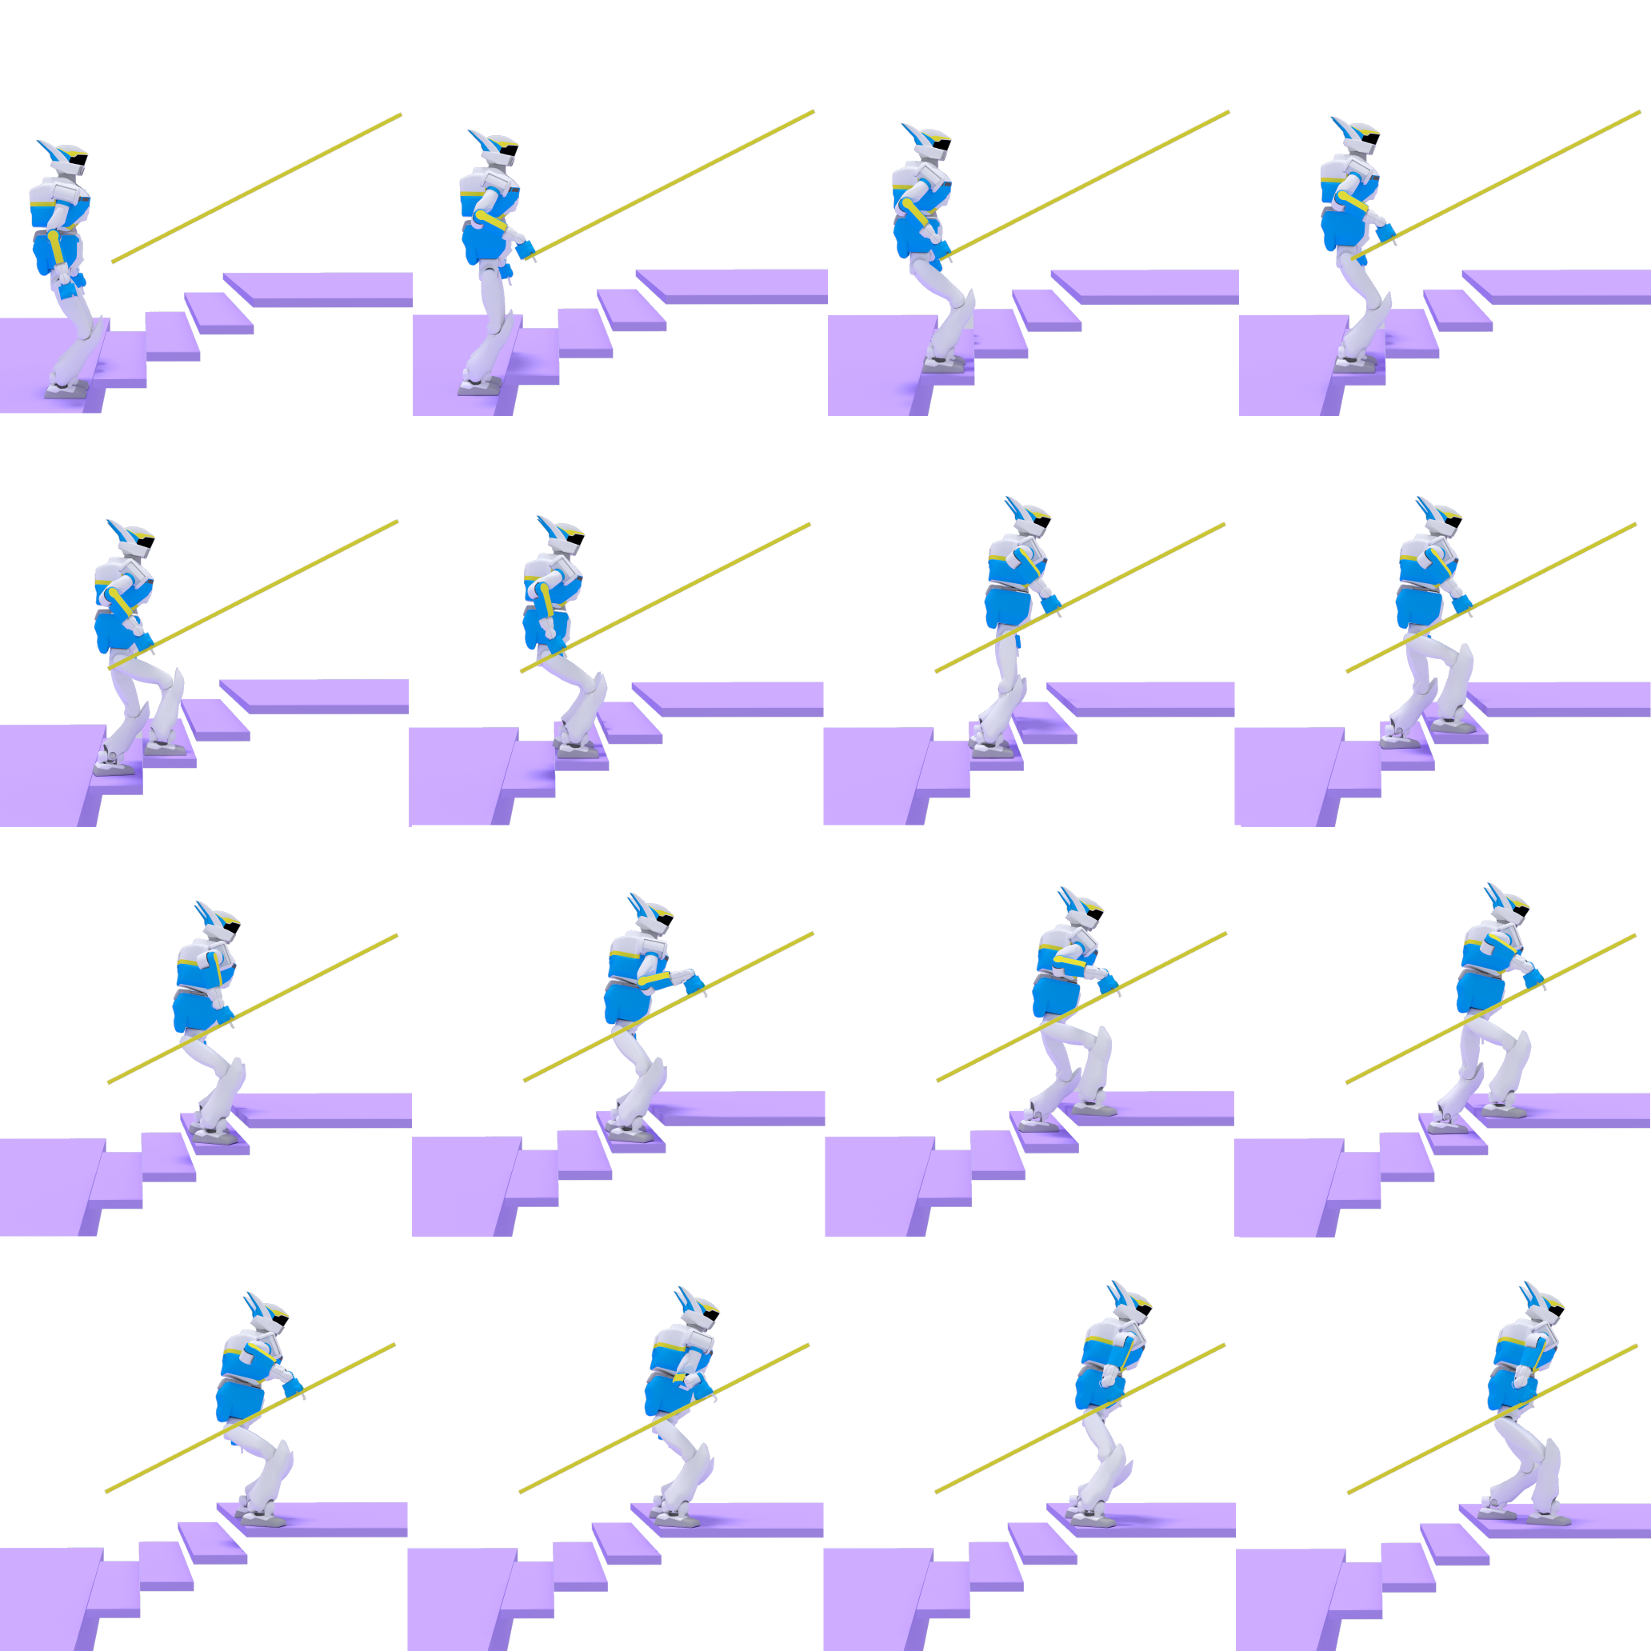
\includegraphics[width=1\linewidth]{figures/stair}
%DIFDELCMD <   %%%
%DIFDELCMD < \caption{%
{%DIFAUXCMD
\DIFdelFL{HRP-2 in the steep stair climbing scenario. }}
		   %DIFAUXCMD
%DIFDELCMD < \label{fig:stair_robust}
%DIFDELCMD < \end{figure}
%DIFDELCMD < 

%DIFDELCMD < %%%
\DIFdel{The goal is to climb three 15-cm high steps.
}%DIFDELCMD < 

%DIFDELCMD < \noindent%%%
\DIFdel{\textbf{Contacts involved:} Feet and right arm.
}%DIFDELCMD < 

%DIFDELCMD < \noindent%%%
\DIFdel{\textbf{Heuristics:} The manipulability $h_w$ is chosen for the feet; $h_{\textrm{\it EFORT}}$ is chosen for the right arm.
%DIF < ~ Regarding equilibrium, the video demonstrates two sequences computed for two different threshold values of $b_0$: $0$ and $2$ (Figure~\ref{fig:stair_robust}). 
}%DIFDELCMD < 

%DIFDELCMD < %%%
%DIF < ~ \noindent\textbf{Observations:}
%DIF < ~ This scenario illustrates best the importance of the equilibrium-robustness criterion.
%DIF < ~ With a robust approach, more states are required to reach the last step (15 rather than 13 in average).
%DIF < ~ However, when the last step is reached by both feet, in the nonrobust case the contacts are extremely close to 
%DIF < ~ the cone limits (Figure~\ref{fig:stair_comp}).
%DIF < ~ 
%DIF < ~ 
%DIF < ~ The geometry of the environment is easily addressed by our planner, and the contact planning is several times faster than real time in this scenario.
%DIF < ~ 
%DIF < ~ Again, the interpolation motion between the contact steps is out of the scope of this paper. However it should be noted that the computed plan in this scenario has been executed successfully on the robot (\url{http://youtu.be/YjL-DBQgXwk#t=0m28s}).
%DIF < ~ 
%DIF < ~ \begin{figure}
  %DIF < ~ \centering
  %DIF < ~ \begin{overpic}[width=0.5\linewidth]{figures/stair_robust}
		%DIF < ~ \put (17,5) {\small{\color{red}$b_0 = 0.23$}} 
		%DIF < ~ \put (79,5) {\small{\color{green}$b_0 = 6.16$}} 
	%DIF < ~ \end{overpic}
  %DIF < ~ \caption{
           %DIF < ~ Evaluation of the robustness $b_0$ of two contact configurations. Although in equilibrium, the left configuration is on the verge of slipping.}
		   %DIF < ~ \label{fig:stair_comp}
%DIF < ~ \end{figure}
%DIFDELCMD < 

%DIFDELCMD < %%%
\DIFdelend \subsubsection{HRP-2 -- Standing up (Figure~\ref{fig:standing})}
From a bent configuration, the robot has to stand up using a wall as support, and climbing a 25-cm high step.

\begin{figure}
  \centering
  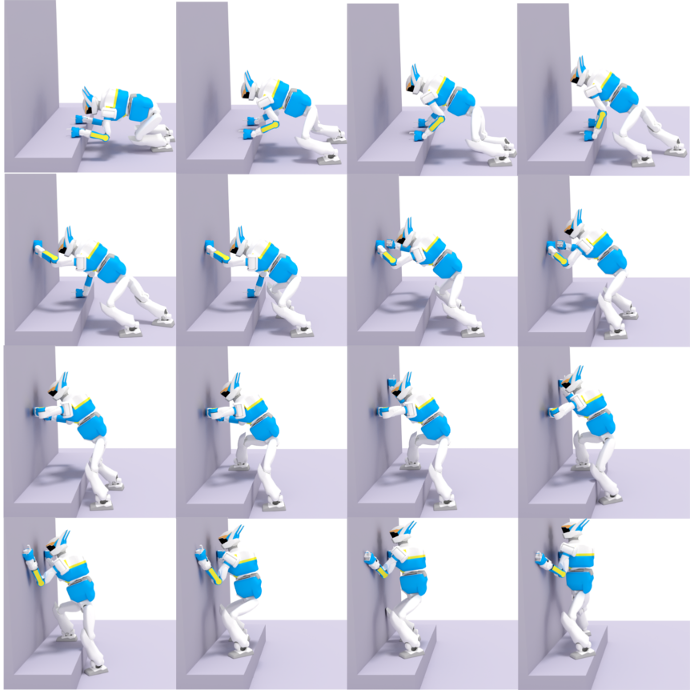
\includegraphics[width=1\linewidth]{figures/standing}
  \caption{
           HRP-2 in the standing scenario. }
		   \label{fig:standing}
\end{figure}


\noindent\textbf{Contacts involved:} All (both feet and hands).

\noindent\textbf{Heuristics:} $h_w$ for the feet, $h_{\textrm{\it EFORT}}$  for the hands.

%~ \noindent\textbf{Observations:} The scenario illustrates well the acyclic aspect of the planning. For instance, in the four first frames of Figure~\ref{fig:standing}, we can see that the right foot
%~ is moved twice, with the left foot in between, before the configuration allows HRP-2 to move its hand.
%~ Because the contacts are tried in a FIFO manner, the fact that the output contact sequence is acyclic shows that a cyclic approach (with a finite state machine for instance) is not sufficient
%~ for the computed path. The reason for this is not reachability, but equilibrium. The planning is slower than for the stair scenario (because the contact generation fails more),
%~ though it remains compatible with \gls{interactive} performances. % \adnote{Maybe define what you mean by 'interactive' and 'real-time' at some point.}


\subsubsection{HRP-2 -- Car egress (Figure~\ref{fig:car})}
In this scenario inspired from the DRC car egress HRP-2 has to step out of a car.

\begin{figure}
  \centering
  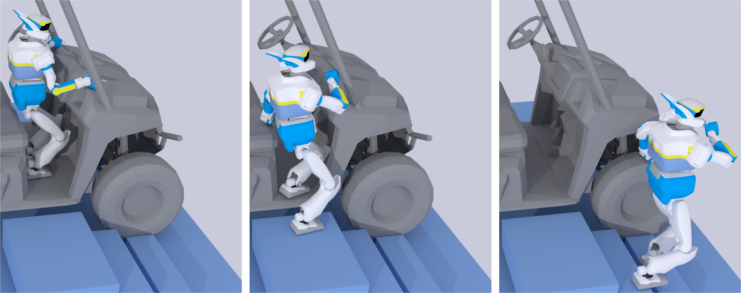
\includegraphics[width=1\linewidth]{figures/polaris}
  \caption{
           Selected frames from the car egress scenario. }
		   \label{fig:car}
\end{figure}


\noindent\textbf{Contacts involved:} All (both feet and hands).

\noindent\textbf{Heuristics:} $h_w$.

%~ \noindent\textbf{Observations:} The difficulty of this scenario lies in the strong reduction of the reachable workspace induced 
%~ by the extreme proximity of all obstacles. The planner is able to find a sequence, that consists in many steps.
%~ The proximity of the obstacles invalidate a large number of contact candidates because of collisions. To avoid breaking more than one contact between each step, the motion has to be decomposed into a large number of steps (61 in average).
%~ While this scenario is the slowest to solve, the planner still computes a solution \glslink{interactive}{interactively}.

\subsubsection{HRP-2 -- Staircase with high steps (Figure~\ref{fig:stair_robust})}
\newcommand{\widthValue}{0.13\linewidth}

\begin{figure*}[h!t!]
  \begin{center}
  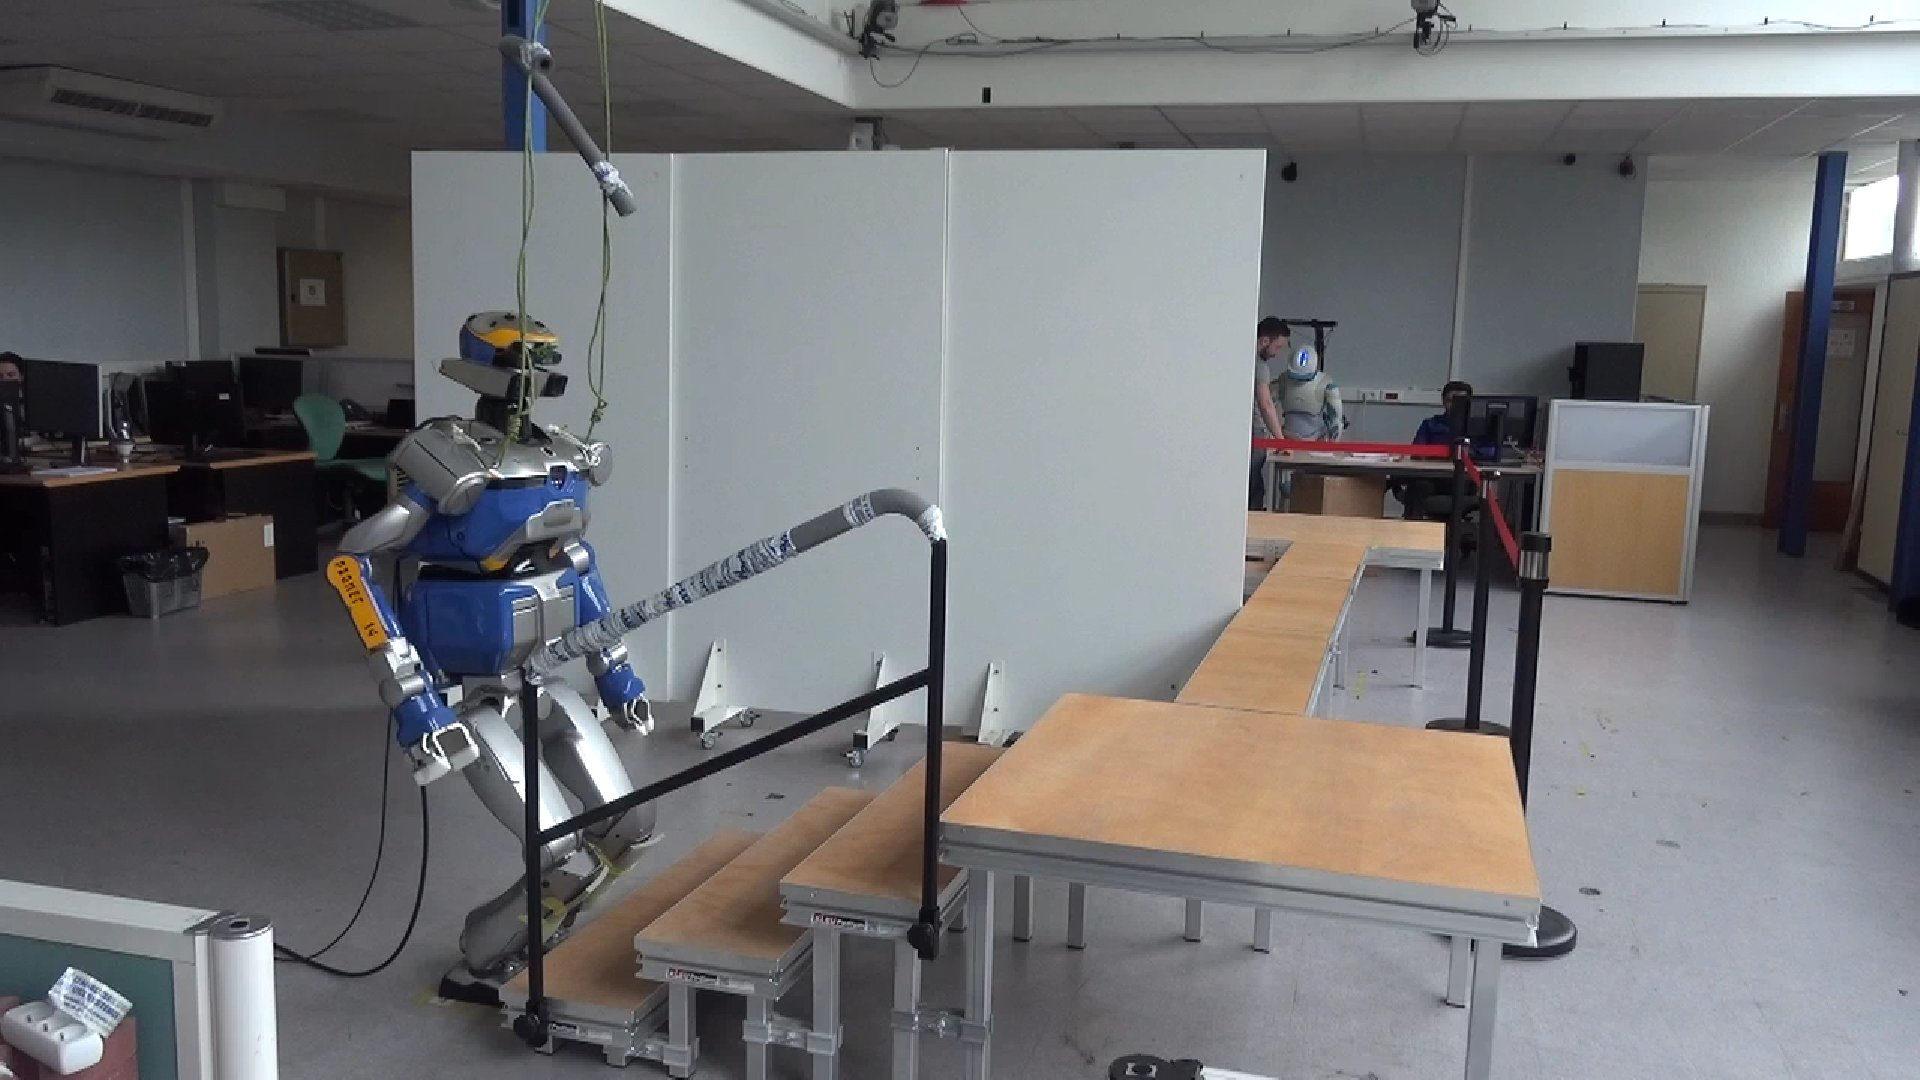
\includegraphics[trim={7.0cm 0.0cm 20.0cm 0.0cm}, clip, width=\widthValue]
    {./video/stairclimbing1.jpeg}
  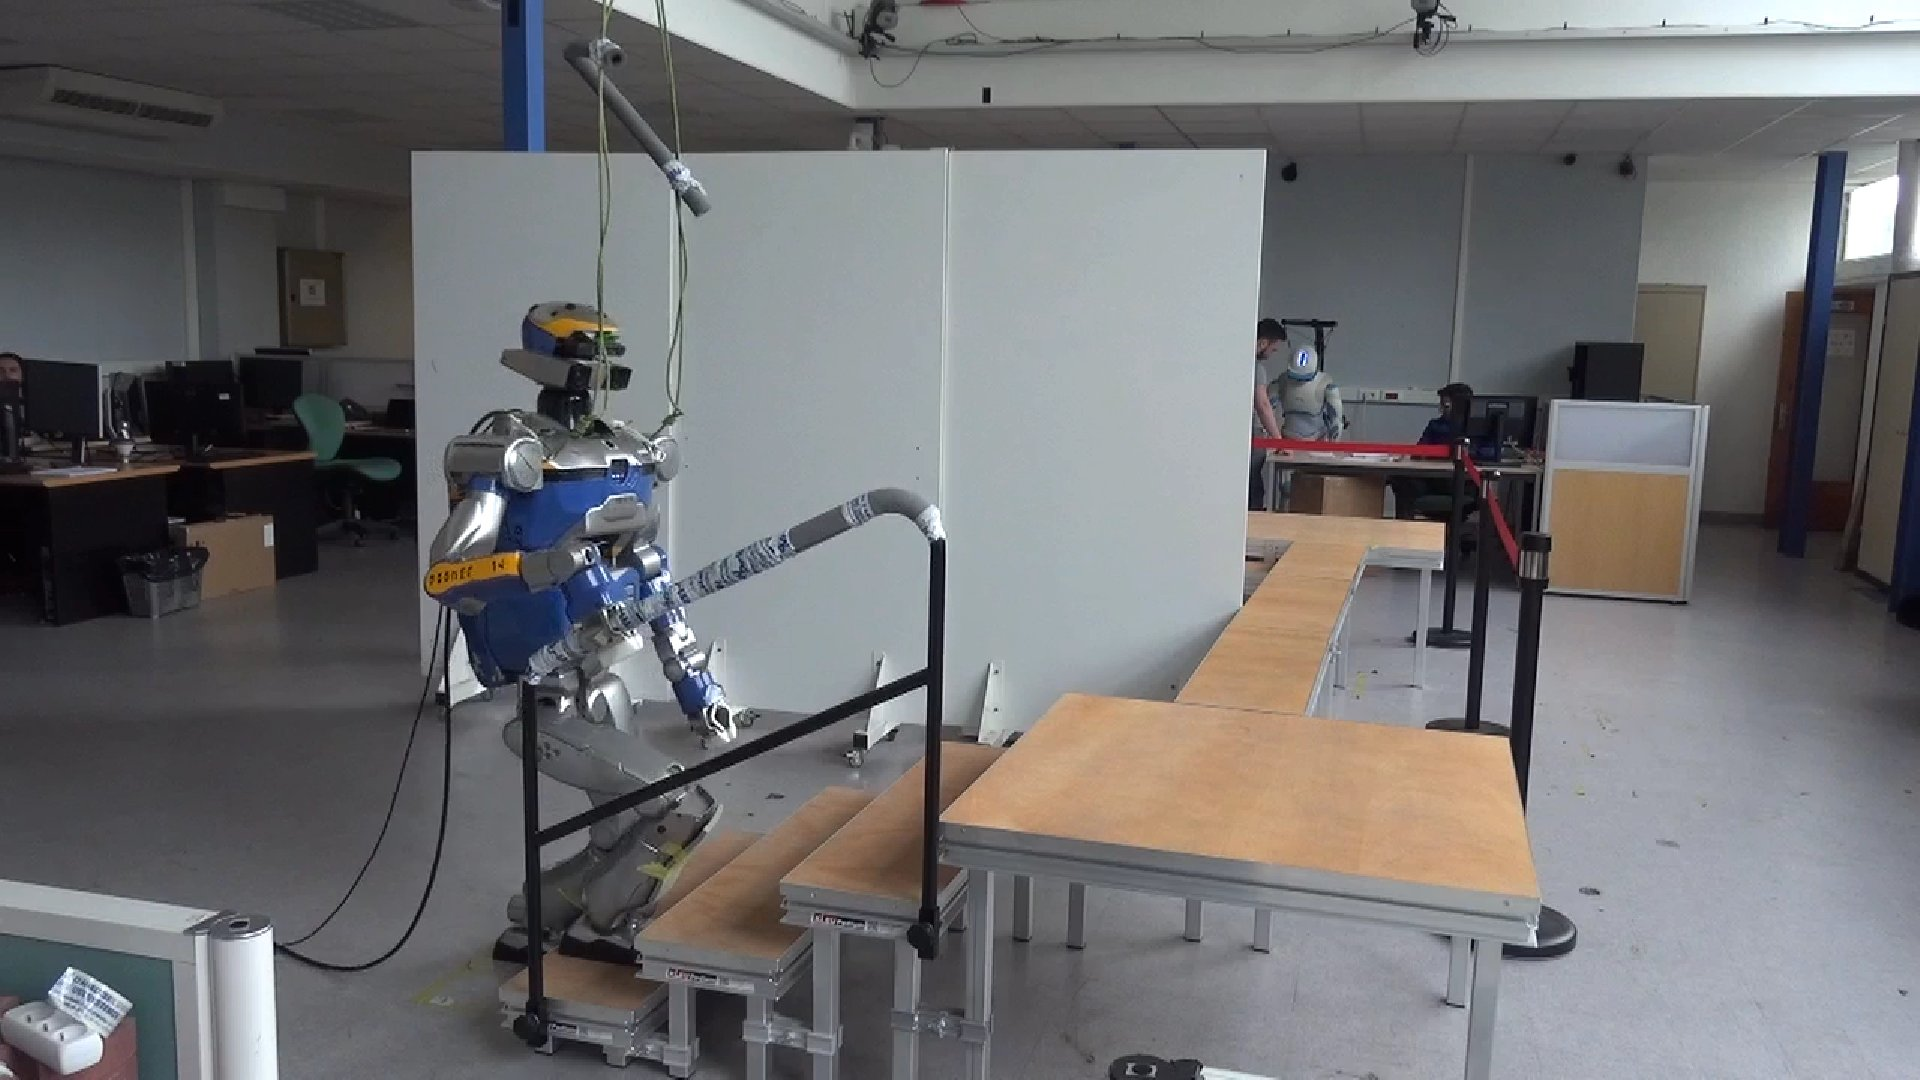
\includegraphics[trim={7.0cm 0.0cm 20.0cm 0.0cm}, clip, width=\widthValue]
    {./video/stairclimbing2.jpeg}
  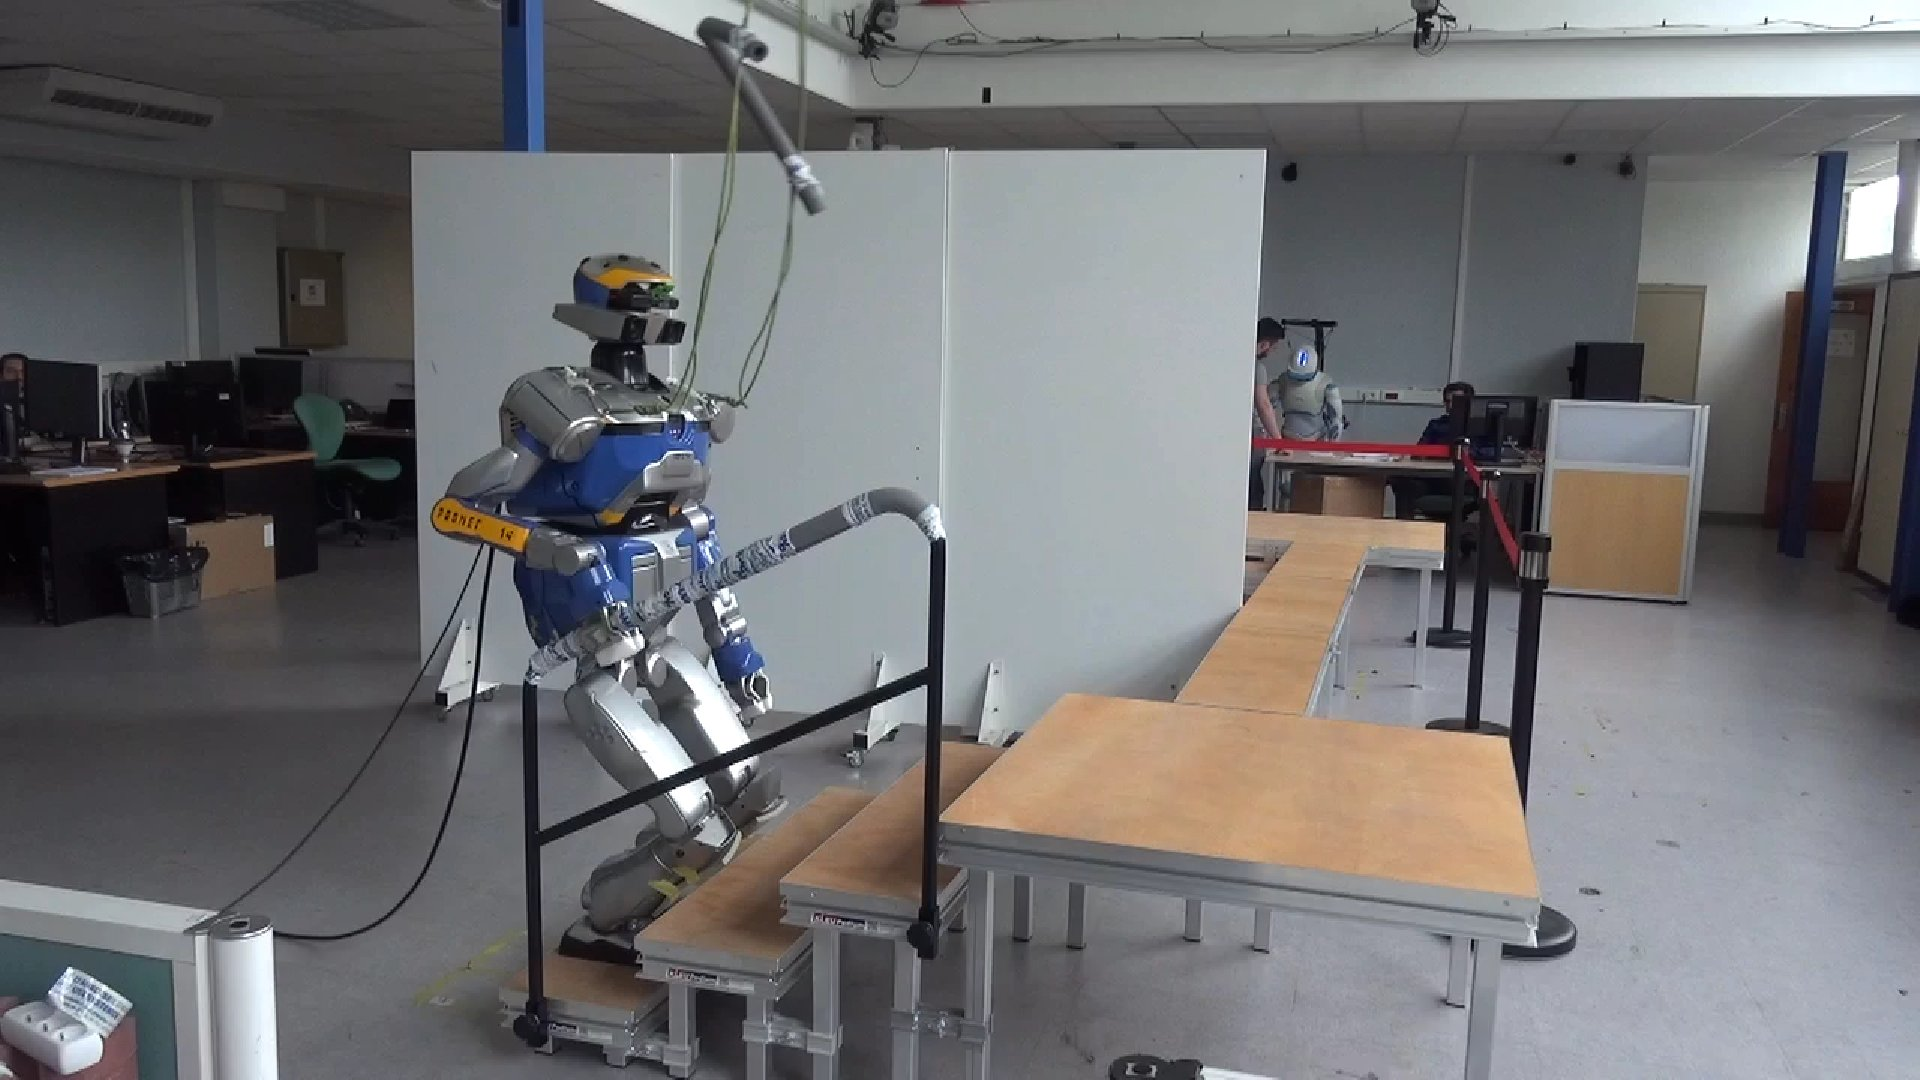
\includegraphics[trim={7.0cm 0.0cm 20.0cm 0.0cm}, clip, width=\widthValue]
    {./video/stairclimbing3.jpeg}
  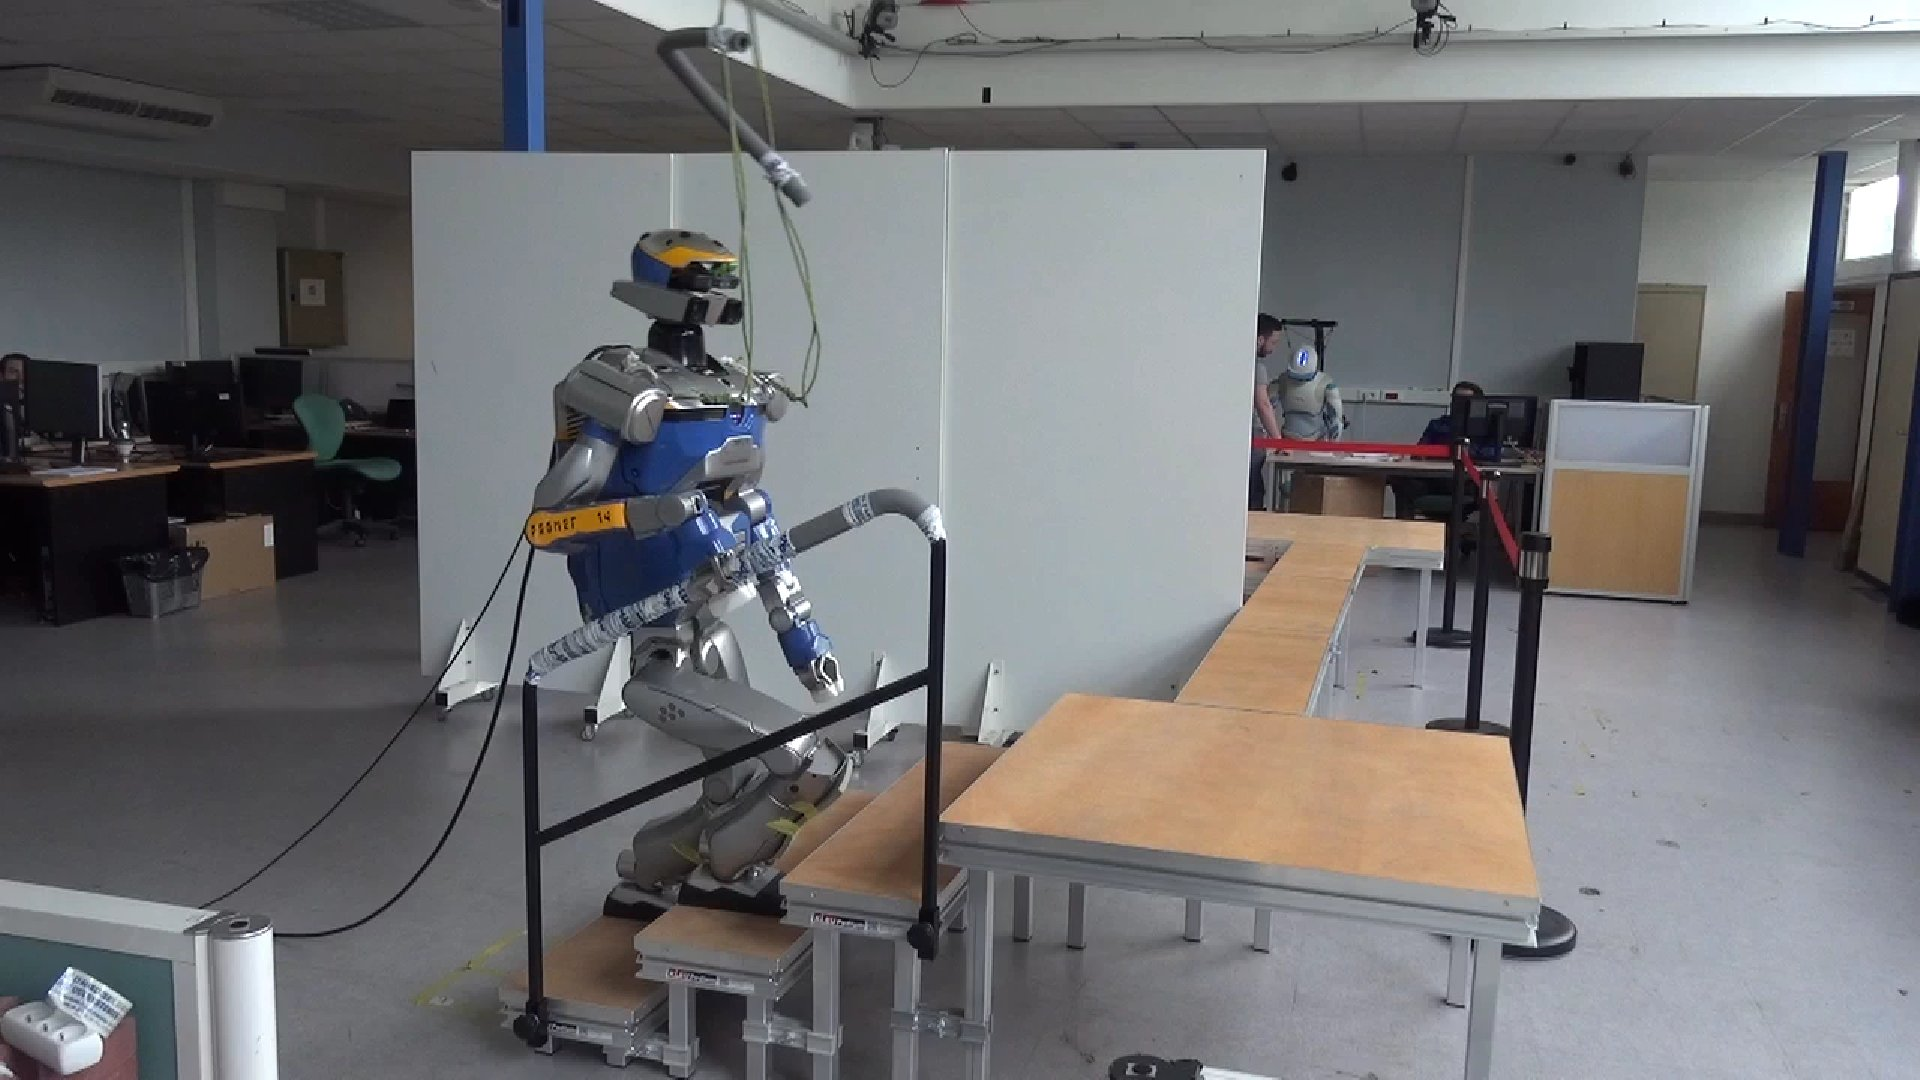
\includegraphics[trim={7.0cm 0.0cm 20.0cm 0.0cm}, clip, width=\widthValue]
    {./video/stairclimbing4.jpeg}
  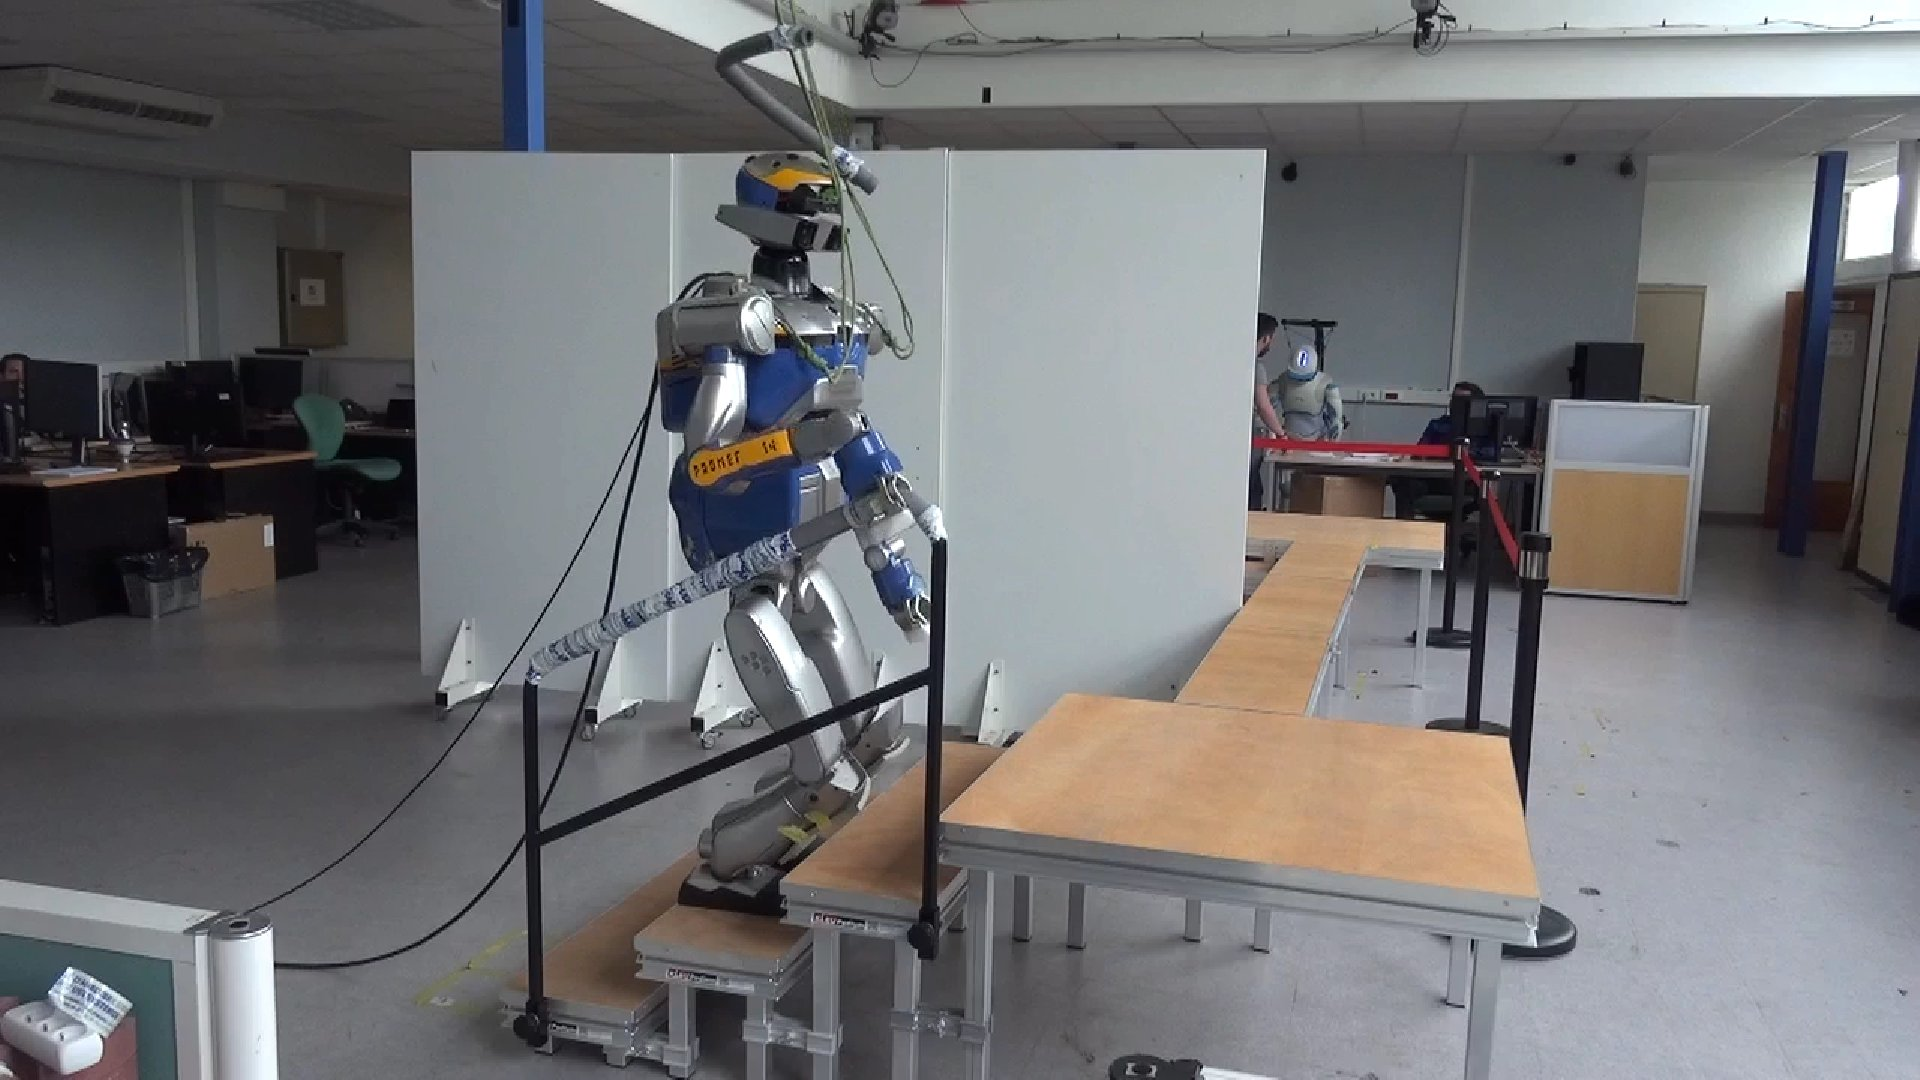
\includegraphics[trim={7.0cm 0.0cm 20.0cm 0.0cm}, clip, width=\widthValue]
    {./video/stairclimbing5.jpeg}
  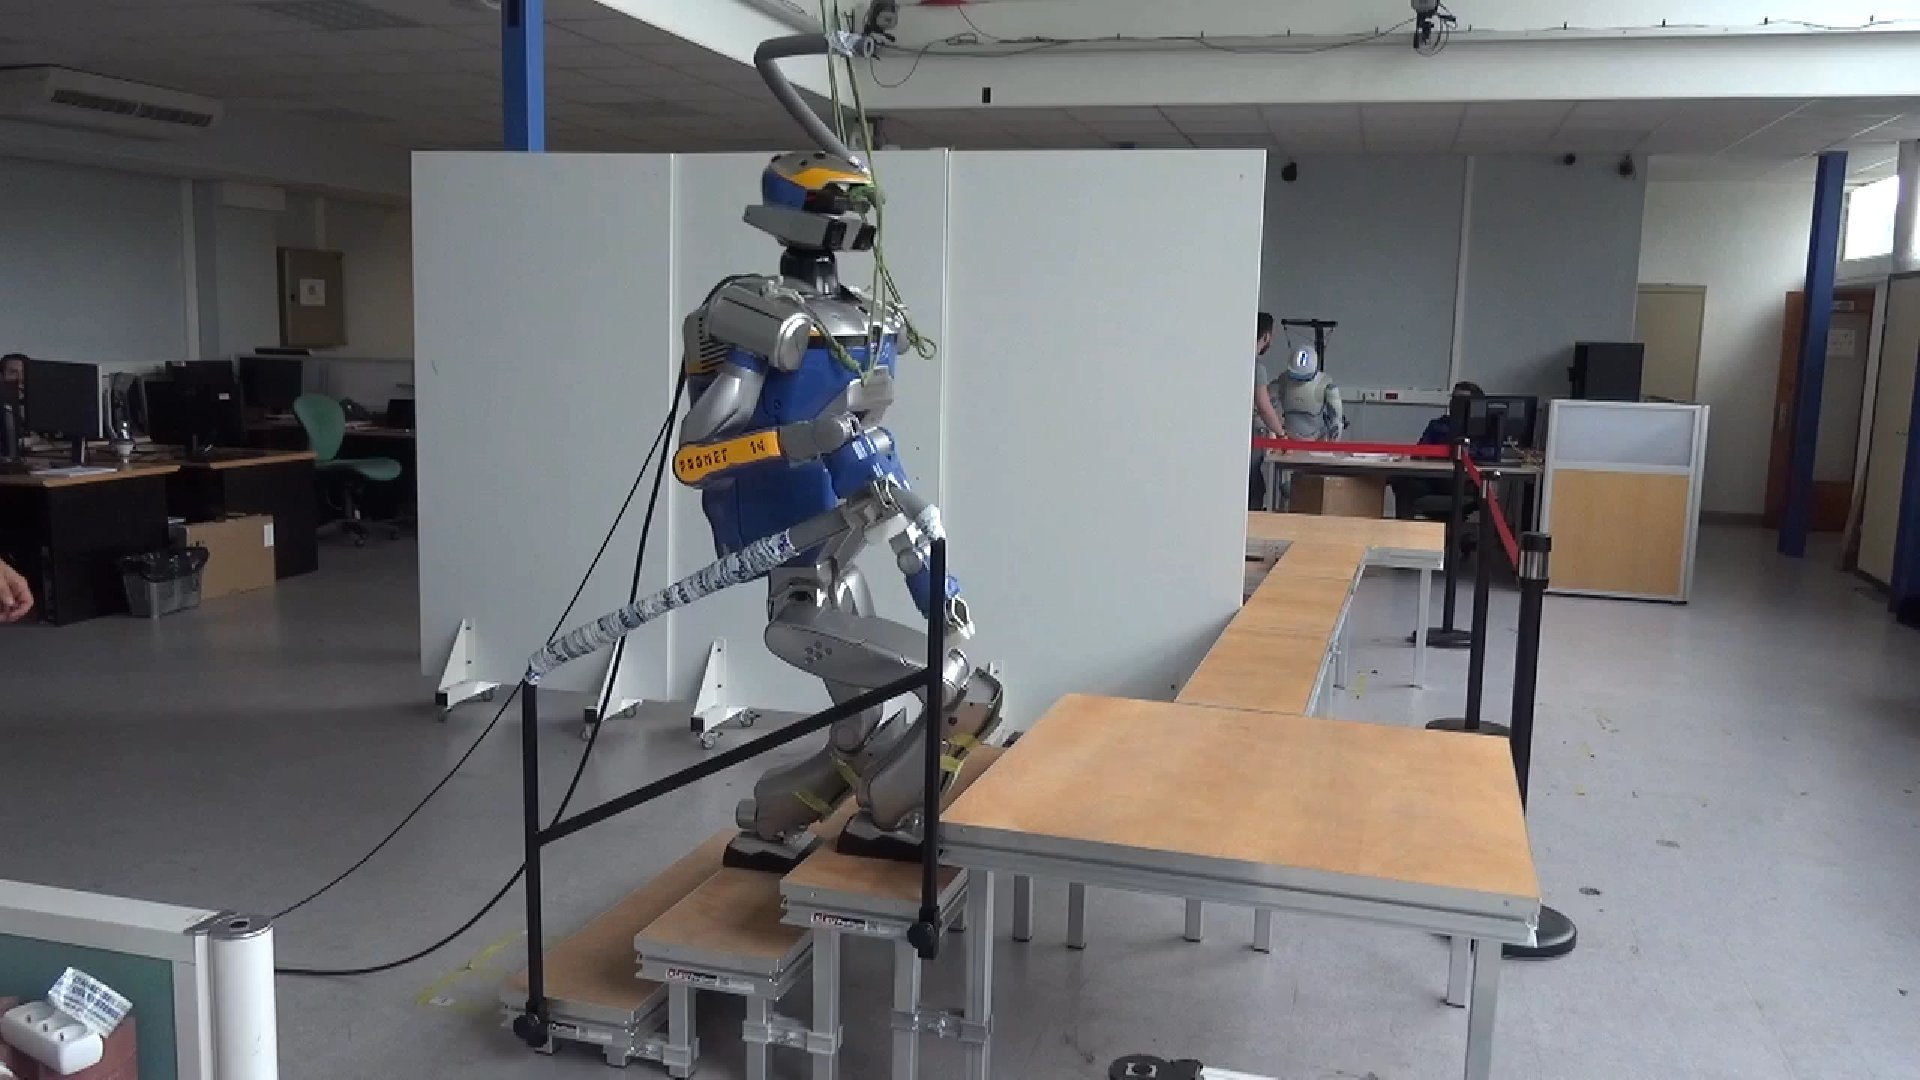
\includegraphics[trim={7.0cm 0.0cm 20.0cm 0.0cm}, clip, width=\widthValue]
    {./video/stairclimbing6.jpeg}
  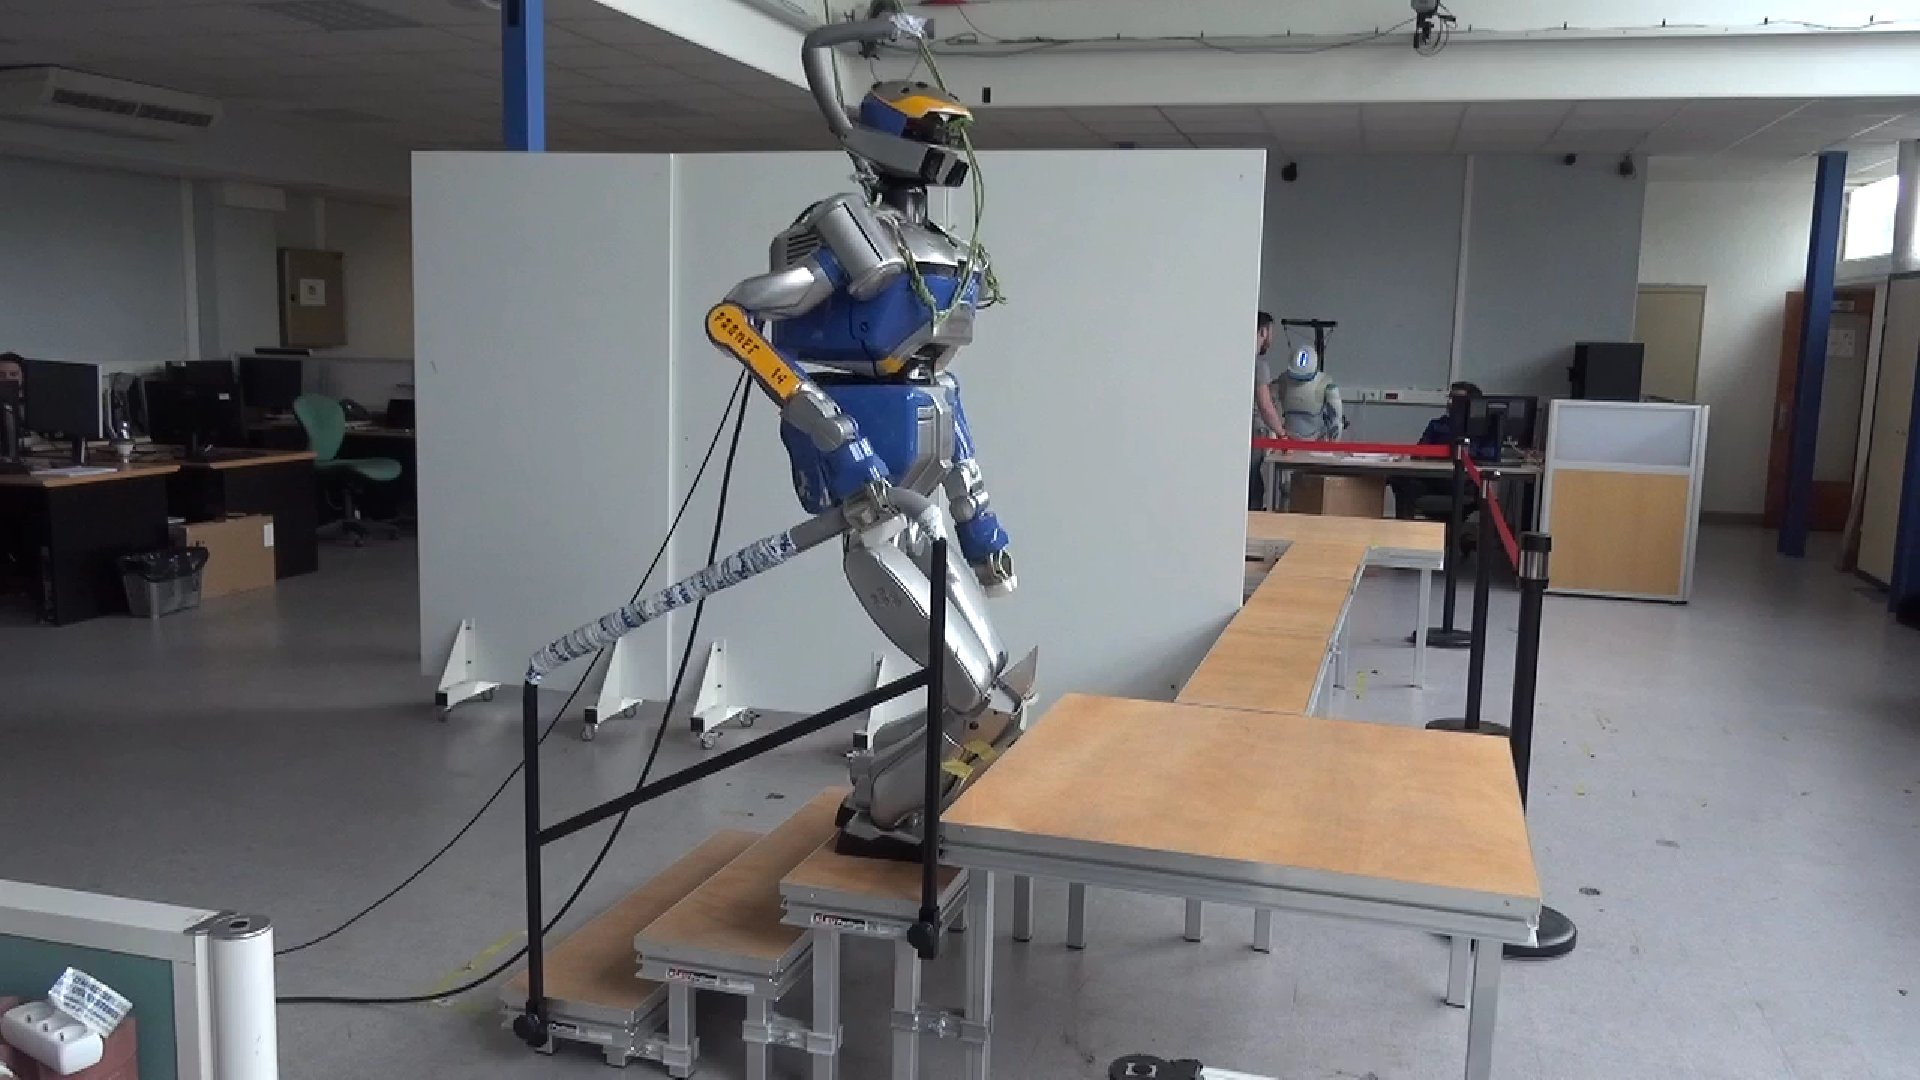
\includegraphics[trim={7.0cm 0.0cm 20.0cm 0.0cm}, clip, width=\widthValue]
    {./video/stairclimbing7.jpeg}
  \caption{
           HRP-2 in the stair climbing scenario. }
		   \label{fig:stair_robust}
  \end{center}
  \vspace{-0.5cm}
\end{figure*}

%DIF > ~ \begin{figure}
  %DIF > ~ \centering
  %DIF > ~ 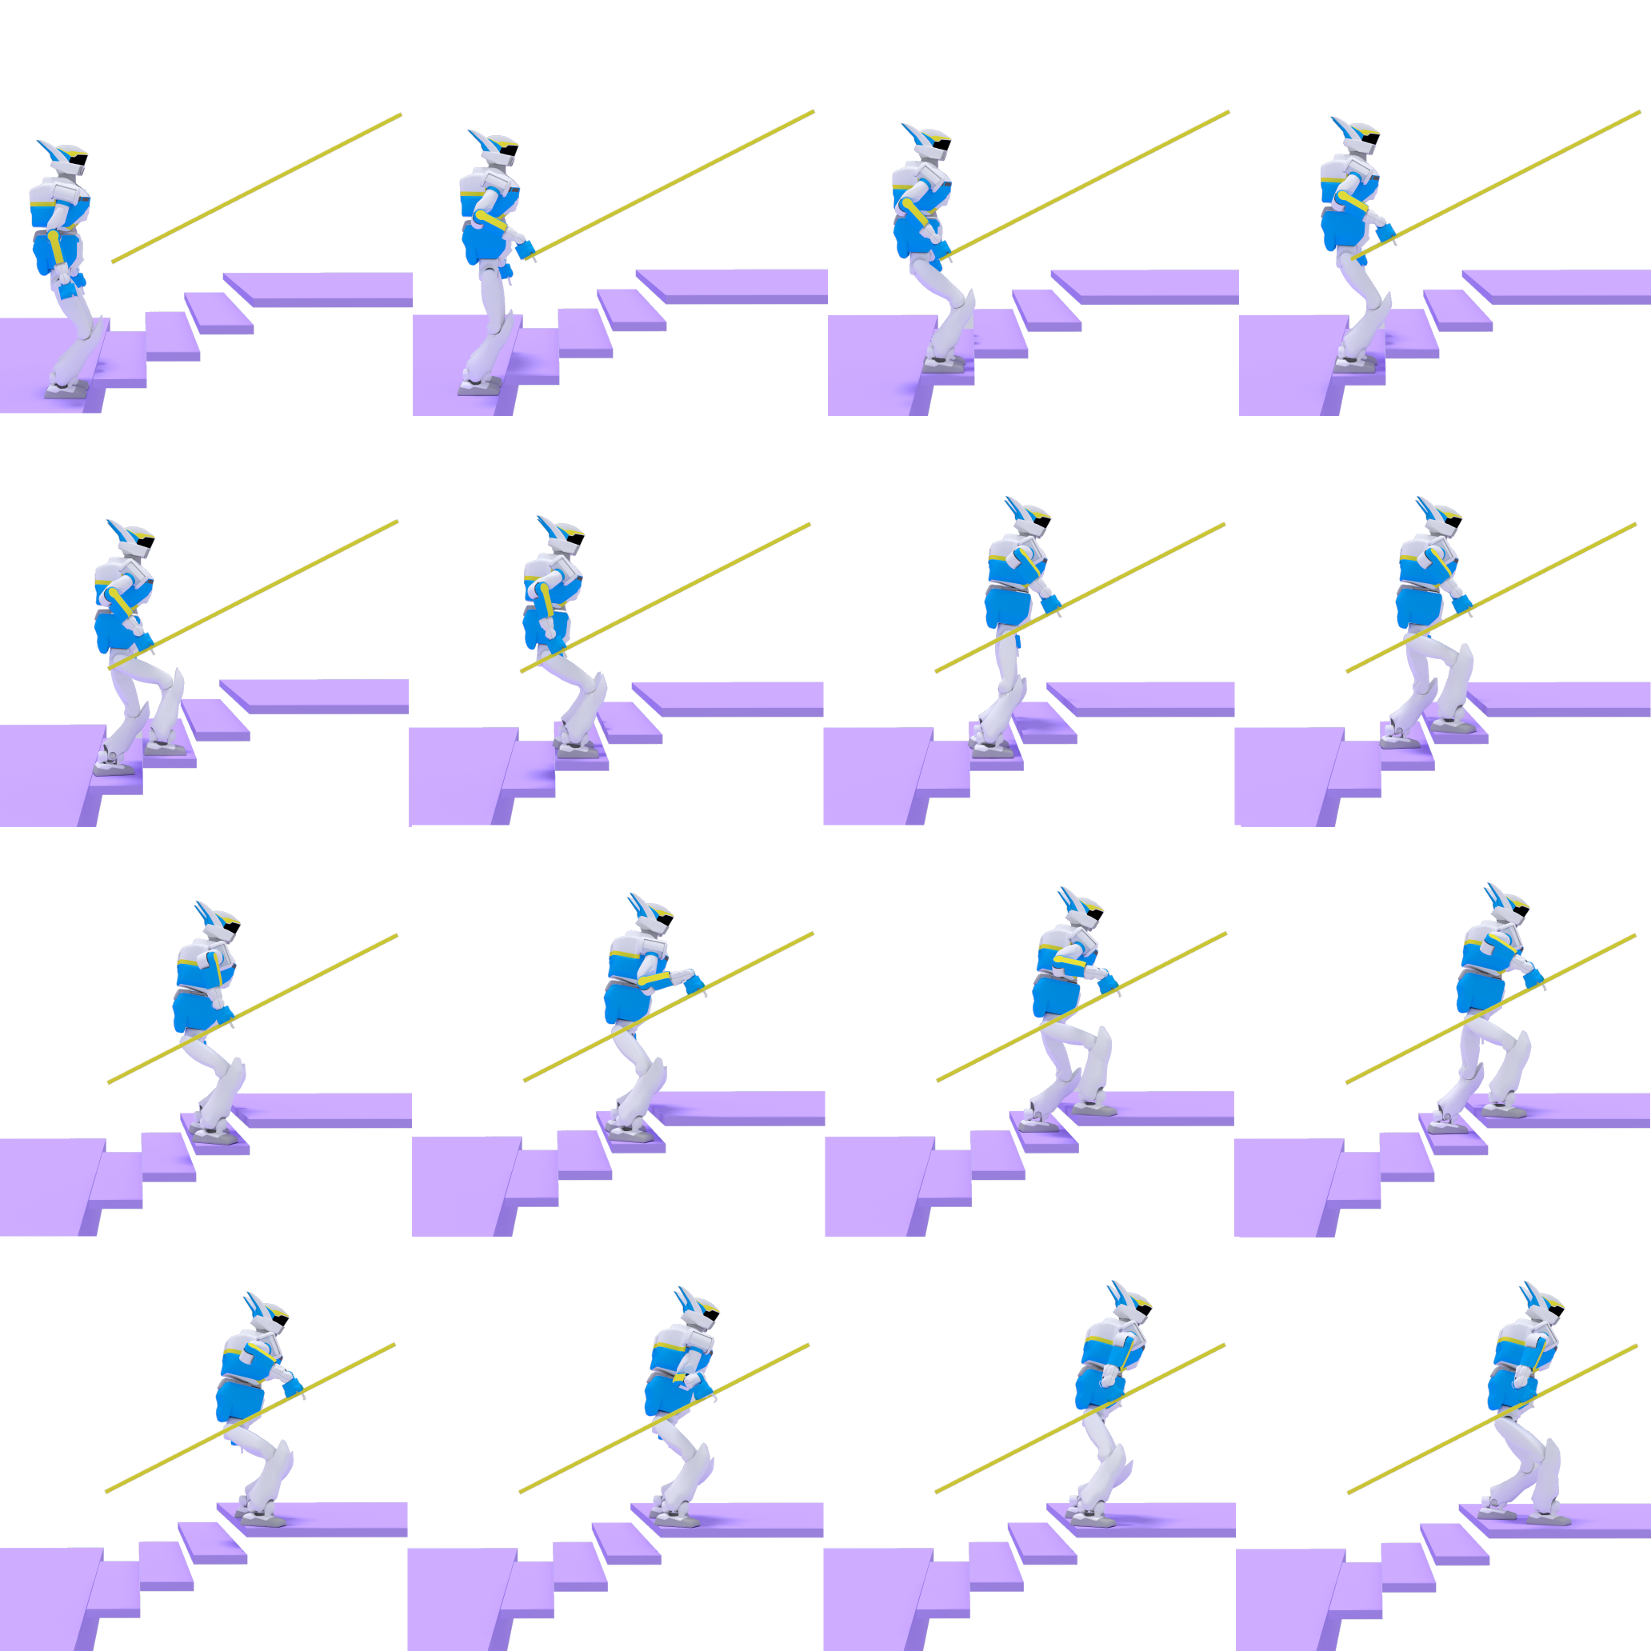
\includegraphics[width=1\linewidth]{figures/stair}
  %DIF > ~ \caption{
           %DIF > ~ HRP-2 in the stair climbing scenario. }
		   %DIF > ~ \label{fig:stair_robust}
%DIF > ~ \end{figure}

\DIFadd{The goal is to climb three 15-cm high steps.
}

\noindent\DIFadd{\textbf{Contacts involved:} Feet and right arm.
}

\noindent\DIFadd{\textbf{Heuristics:} The manipulability $h_w$ is chosen for the feet; $h_{\textrm{\it EFORT}}$ is chosen for the right arm.
%DIF > ~ Regarding equilibrium, the video demonstrates two sequences computed for two different threshold values of $b_0$: $0$ and $2$ (Figure~\ref{fig:stair_robust}). 
}

%DIF > ~ \noindent\textbf{Observations:}
%DIF > ~ This scenario illustrates best the importance of the equilibrium-robustness criterion.
%DIF > ~ With a robust approach, more states are required to reach the last step (15 rather than 13 in average).
%DIF > ~ However, when the last step is reached by both feet, in the nonrobust case the contacts are extremely close to 
%DIF > ~ the cone limits (Figure~\ref{fig:stair_comp}).
%DIF > ~ 
%DIF > ~ 
%DIF > ~ The geometry of the environment is easily addressed by our planner, and the contact planning is several times faster than real time in this scenario.
%DIF > ~ 
%DIF > ~ Again, the interpolation motion between the contact steps is out of the scope of this paper. However it should be noted that the computed plan in this scenario has been executed successfully on the robot (\url{http://youtu.be/YjL-DBQgXwk#t=0m28s}).
%DIF > ~ 
%DIF > ~ \begin{figure}
  %DIF > ~ \centering
  %DIF > ~ \begin{overpic}[width=0.5\linewidth]{figures/stair_robust}
		%DIF > ~ \put (17,5) {\small{\color{red}$b_0 = 0.23$}} 
		%DIF > ~ \put (79,5) {\small{\color{green}$b_0 = 6.16$}} 
	%DIF > ~ \end{overpic}
  %DIF > ~ \caption{
           %DIF > ~ Evaluation of the robustness $b_0$ of two contact configurations. Although in equilibrium, the left configuration is on the verge of slipping.}
		   %DIF > ~ \label{fig:stair_comp}
%DIF > ~ \end{figure}


\DIFaddend \subsubsection{HyQ -- DRC-style rubble (Figure~\ref{fig:darpa})}
The quadruped robot must cross a rubble composed of bricks rotated at different angles and directions.

\begin{figure}
  \centering
  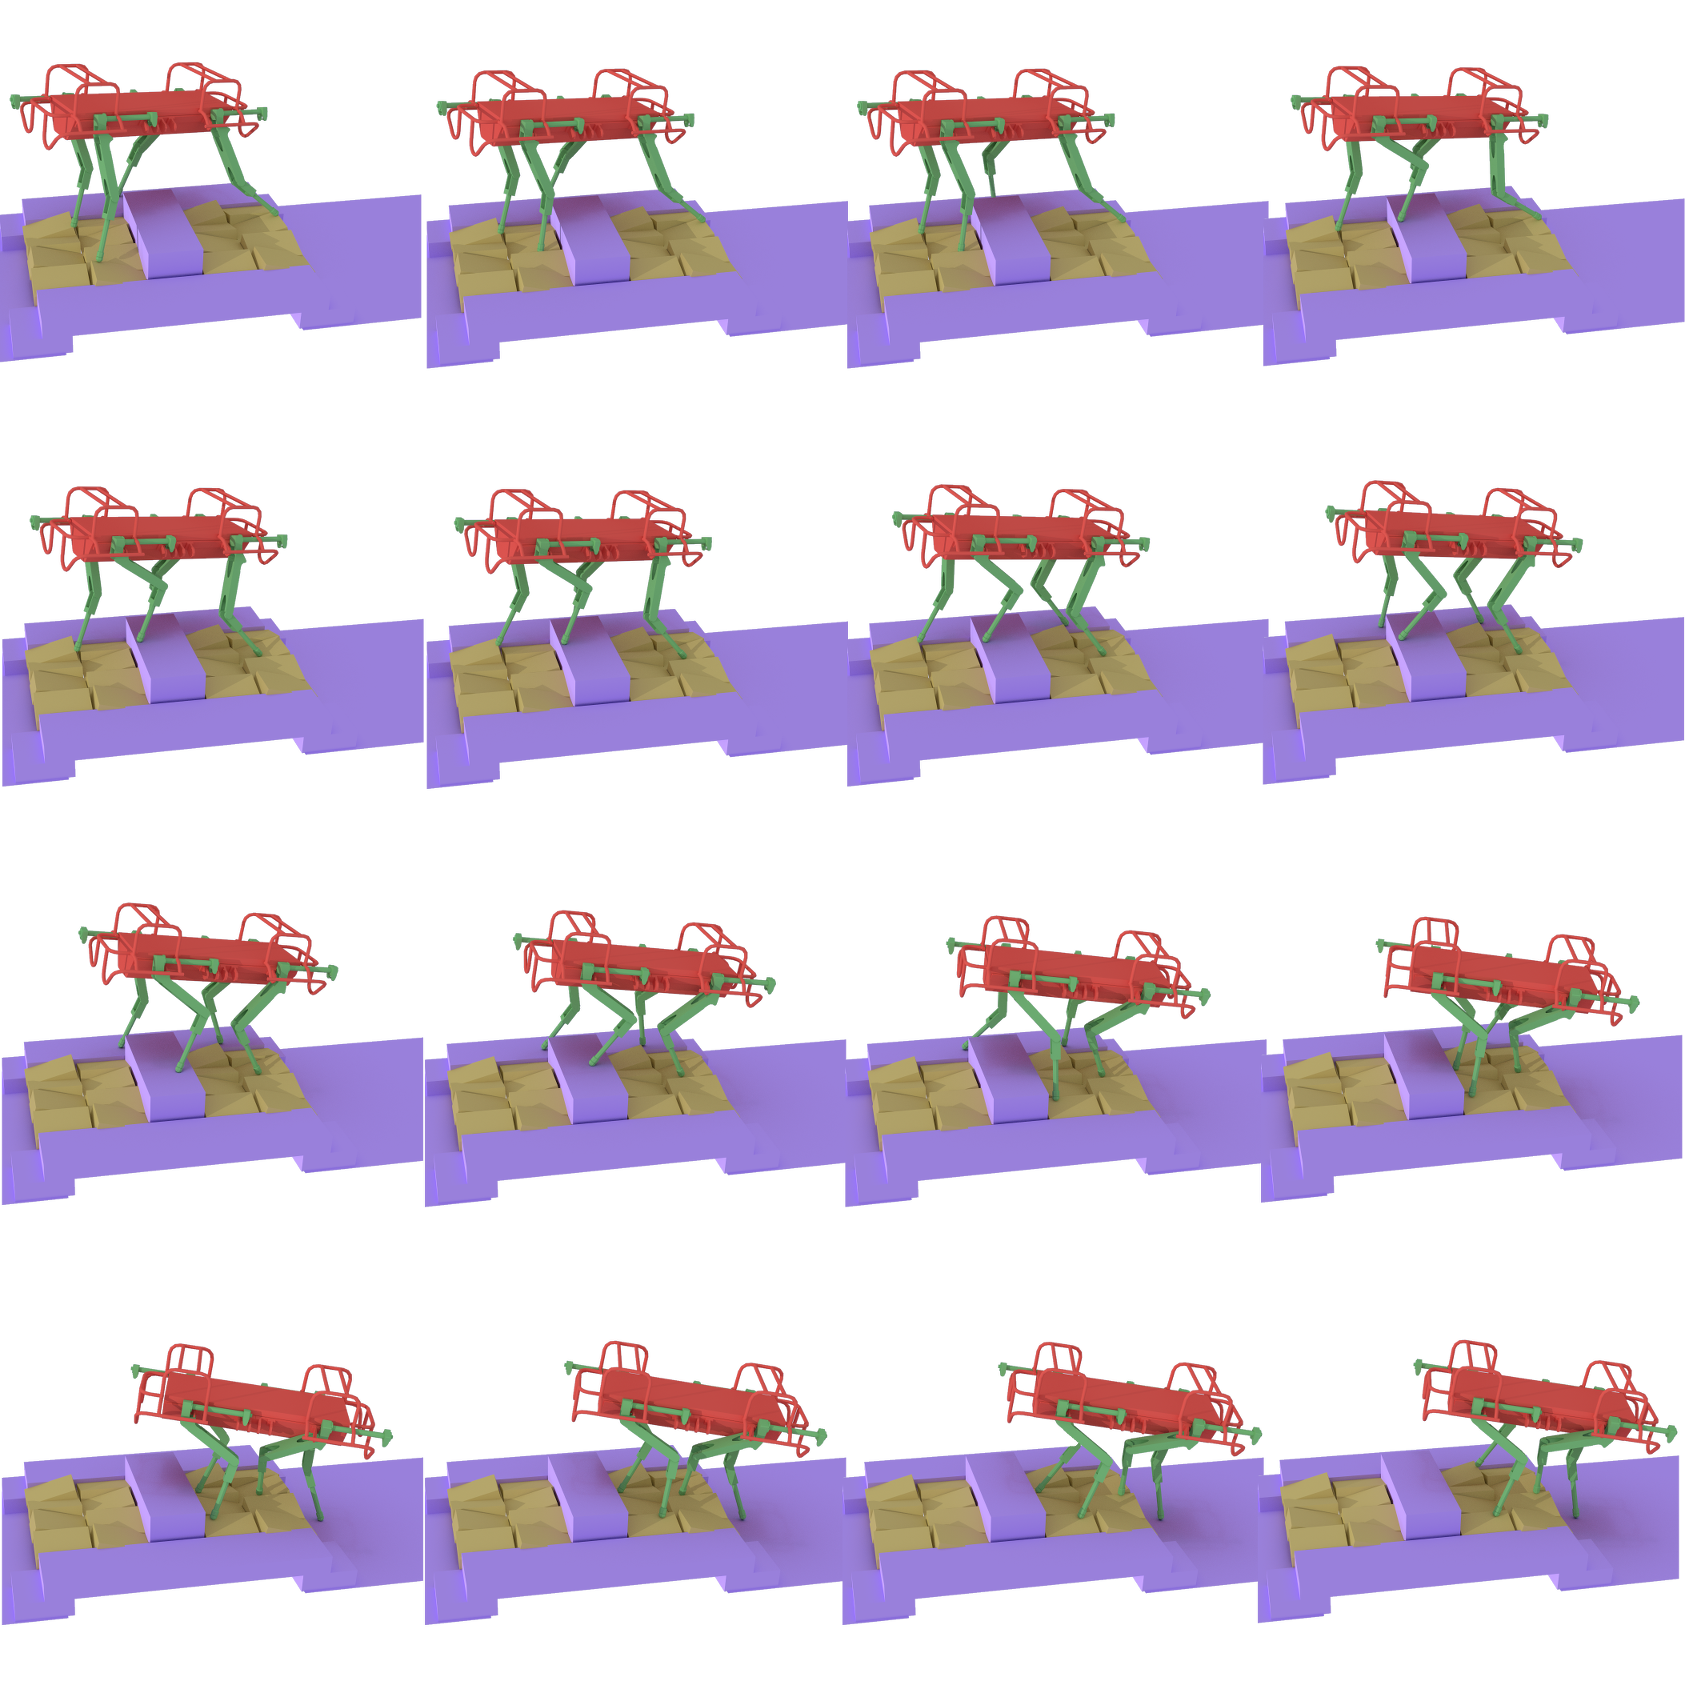
\includegraphics[width=1\linewidth]{figures/darpa}
  \caption{
           Robust crossing of rubbles by HyQ. }
		   \label{fig:darpa}
\end{figure}


\noindent\textbf{Contacts involved:} All (the 4 legs).

\noindent\textbf{Heuristics:} $h_w$ for all legs. The robustness threshold $b_0$ is set to $20$.

%~ \noindent\textbf{Observations:} In this context, setting up a really important minimum value for $b_0$ is possible due to the high
%~ stability of the HyQ robot, and results in more contact switches, in exchange for safety. The guide path-planning in this scenario takes a few seconds in average, more than
%~ in any other scenarios. This is explained by the necessity of discovering a safe way to ``climb down'' the rubble. In this part of the planning, the constraint that the 4 reachable workspaces of all legs must collide with the environment at all times is hard to respect, but enforces the equilibrium of HyQ. %\adnote{Why do not relax this constraint and require only 3 legs?} 
%~ Again, the computation times remain however \gls{interactive}.

\subsubsection{HyQ -- Obstacle race (Figure~\ref{fig:HyQ_bridge} and~\ref{fig:HyQ_obs})}
In this long scene, HyQ has to cross a 55-cm large hole, followed by a narrow ``bridge'', only 25-cm large.

\begin{figure}
  \centering
  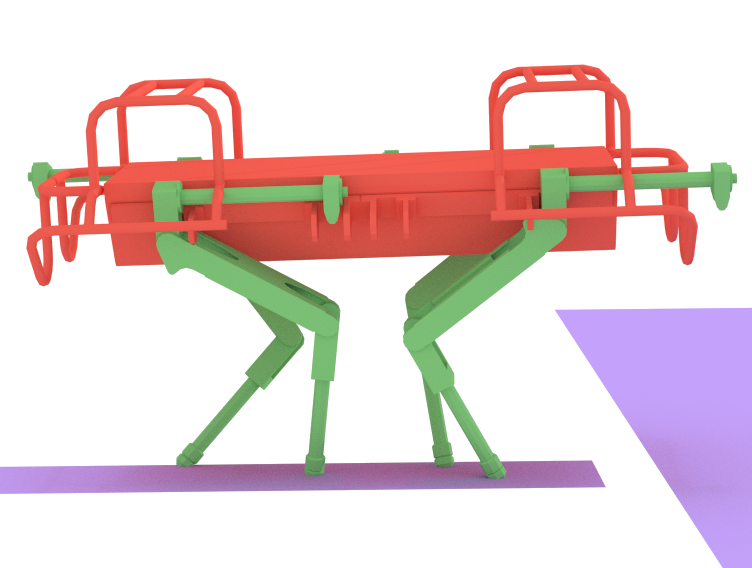
\includegraphics[width=0.4\linewidth]{figures/HyQ_bridge}
  \caption{
           HyQ crossing a narrow bridge. }
		   \label{fig:HyQ_bridge}
\end{figure}

\begin{figure}
  \centering
  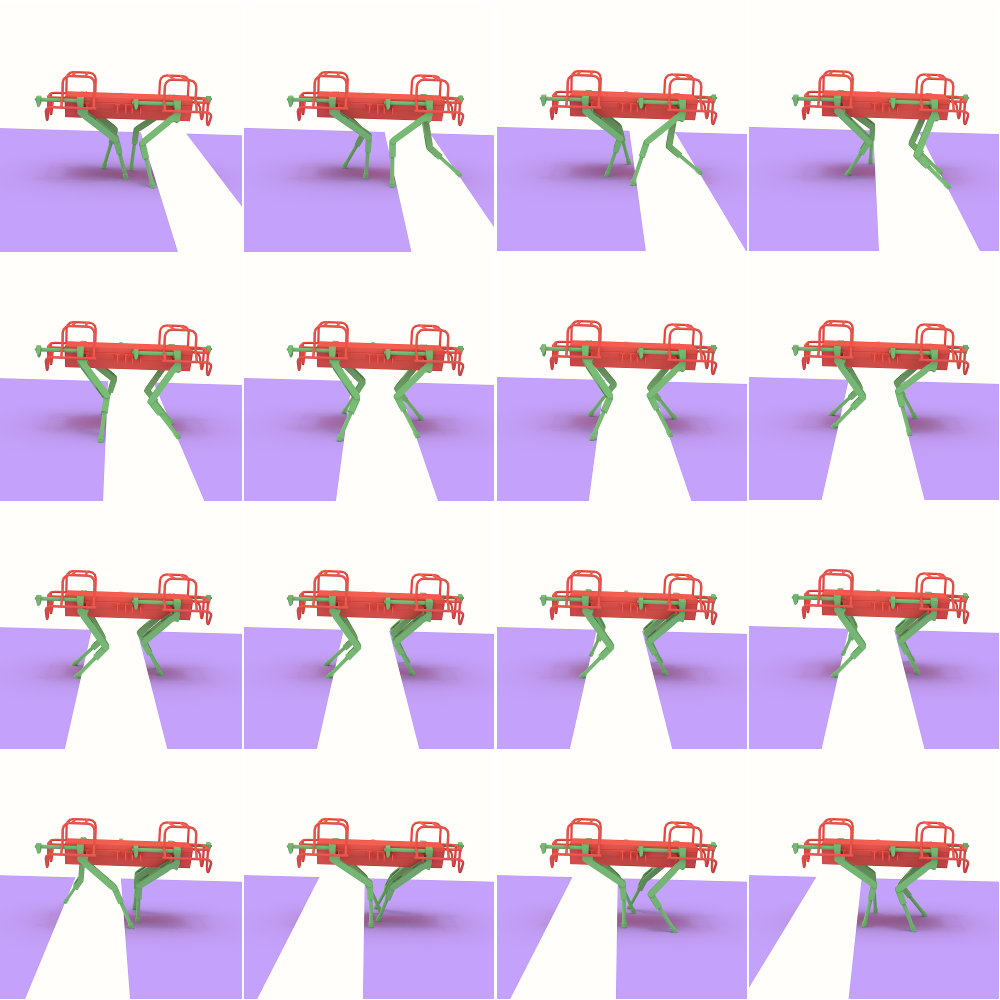
\includegraphics[width=1\linewidth]{figures/HyQ_obs}
  \caption{
           Crossing a hole contact sequence for HyQ. }
		   \label{fig:HyQ_obs}
\end{figure}



\noindent\textbf{Contacts involved:} All (the 4 legs).

\noindent\textbf{Heuristics:} $h_w$ for all legs. The robustness threshold $b_0$ is set to $10$.

%~ \noindent\textbf{Observations:} Despite the apparent simplicity of the scene, this scenario is a hard case for a contact planner.
%~ While finding a guide path above the hole is easy for the guide planner, finding a sequence of contacts that allows for equilibrium is not trivial.
%~ Second, the narrow bridge is hard both for the planner and the contact generator: to make sure that equilibrium is preserved along the traversal,
%~ the bridge must be approached with the appropriate angle.
%~ The difficulty is illustrated in Figure~\ref{fig:HyQ_obs}, where several feet rearrangements are required to cross the hole (although the video shows this best).
%~ The planner however succeeds in finding a feasible sequence in the end, again with \gls{interactive} computation times.

\subsubsection{HRP-2 -- Path re-planning (Figure~\ref{fig:re-planning})}
In this long scene, HRP-2 plans a path through several obstacles. The scene is edited during the execution of the motion: a stair is added,
some stepping stones are removed, and part of the final staircase is deleted. All these modifications require re-planning.


\begin{figure}
  \centering
  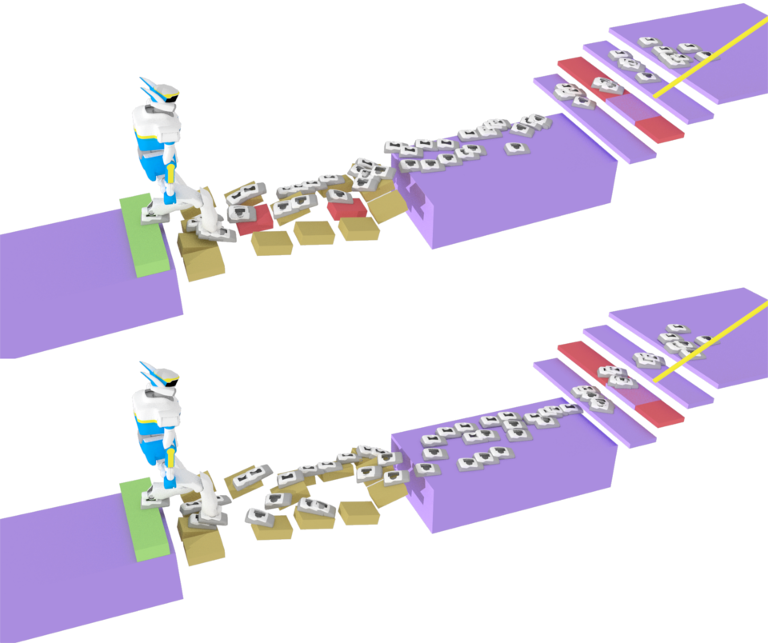
\includegraphics[width=0.7\linewidth]{figures/replanning}
  \caption{
           HRP-2 in the re-planning scenario. After the red step stones are removed, a new sequence of contacts is re-planned. Hand contacts
           are not presented here for readability.}
		   \label{fig:re-planning}
\end{figure}

\noindent\textbf{Contacts involved:} Feet and the right arm.

\noindent\textbf{Heuristics:} $h_w$  for all legs. $h_{\textrm{\it EFORT}}$  for the right arm. The robustness threshold is set to $2$.

%~ \noindent\textbf{Observations:} This scenario is designed to illustrate concretely the computation times of the planner.
%~ In the video, the footsteps indicating the contact sequence appear at the average speed of their computation (including the guide-path planning).


\DIFdelbegin \subsubsection{\DIFdel{3-fingered hand -- Manipulation of a pen (Figure~\ref{fig:penrot})}}
%DIFAUXCMD
\addtocounter{subsubsection}{-1}%DIFAUXCMD
\DIFdel{This scenario is proposed to illustrate the generality of our approach: we consider a manipulation task for a robotic hand and use
our contact planner to compute a contact sequence for the fingers, considered as effectors (Figure~\ref{fig:penrot}).
Although we do not address the hard issue of accounting for rolling motions, the planner is able to compute the shown sequences in less than 5 seconds.
}\DIFdelend %DIF > ~ \subsubsection{3-fingered hand -- Manipulation of a pen (Figure~\ref{fig:penrot})}
%DIF > ~ This scenario is proposed to illustrate the generality of our approach: we consider a manipulation task for a robotic hand and use
%DIF > ~ our contact planner to compute a contact sequence for the fingers, considered as effectors (Figure~\ref{fig:penrot}).
%DIF > ~ Although we do not address the hard issue of accounting for rolling motions, the planner is able to compute the shown sequences in less than 5 seconds.
%DIF > ~ 
%DIF > ~ \begin{figure*}
%DIF > ~ \centering
  %DIF > ~ \begin{overpic}[width=1\linewidth]{figures/penrot}
	%DIF > ~ \end{overpic}
%DIF > ~ \caption{Contact sequence found for a pen manipulation in a zero gravity environment.}
		   %DIF > ~ \label{fig:penrot}
%DIF > ~ \end{figure*}
%DIF > ~ 
 %DIF > ~ 
%DIF > ~ \noindent\textbf{Contacts involved:} Three finger-tips.
%DIF > ~ 
%DIF > ~ \noindent\textbf{Heuristics:} $h_{\textrm{\it EFORT}}$ for all fingers.

 
\DIFdelbegin %DIFDELCMD < \begin{figure*}
%DIFDELCMD < \centering
%DIFDELCMD <   \begin{overpic}[width=1\linewidth]{figures/penrot}
%DIFDELCMD < 	\end{overpic}
%DIFDELCMD < %%%
%DIFDELCMD < \caption{%
{%DIFAUXCMD
\DIFdelFL{Contact sequence found for a pen manipulation in a zero gravity environment.}}
		   %DIFAUXCMD
%DIFDELCMD < \label{fig:penrot}
%DIFDELCMD < \end{figure*}
%DIFDELCMD < 

%DIFDELCMD <  
%DIFDELCMD < \noindent%%%
\DIFdel{\textbf{Contacts involved:} Three finger-tips.
}%DIFDELCMD < 

%DIFDELCMD < \noindent%%%
\DIFdel{\textbf{Heuristics:} $h_{\textrm{\it EFORT}}$ for all fingers.
 }%DIFDELCMD < 

%DIFDELCMD <  
%DIFDELCMD < %%%
\DIFdelend \subsection{Role of the main parameters} \label{sec:influence}
We discuss the factors that influence the outcome of our planner: the root scaling factor $s$ (Section~\ref{sec:scaling}), the heuristics for
contact generation (Appendix~\ref{sec:heuristics}), and lastly, the discretization step for the guide path. The appropriate value for these parameters
is computed empirically based on use-case analysis or trials and errors.

\subsubsection{Choosing the scaling factor $s$} \label{sec:params}
%~ \deladp{To find a convenient value $s^*$ of $s$, we proceeded as follows. }
For several values of $s$, we generated $10 000$ configurations. 
%DIF > ~ We then computed the sensitivity of the reachability condition (percentage of configurations in $C_{Reach}^0$ belonging to \gls{$C_{Contact}^0$}).
%DIF > ~ Similarly we computed the specificity of the condition (percentage of configurations \textbf{not} in $C_{Reach}^0$ \textbf{not} belonging to \gls{$C_{Contact}^0$}).
We then computed the sensitivity \DIFaddbegin \DIFadd{and specificity }\DIFaddend of the reachability condition\DIFdelbegin \DIFdel{(}\DIFdelend \DIFaddbegin \DIFadd{.  In this context, the sensitivity refers to the }\DIFaddend percentage of configurations in $C_{Reach}^0$, effectively belonging to \gls{$C_{Contact}^0$}\DIFdelbegin \DIFdel{). Similarly we computed the specificity of the condition (}\DIFdelend \DIFaddbegin \DIFadd{. If a sampled configuration is in $C_{Reach}^0$, but our method is unable to generate a contact configuration from it, as a result the sensitivity
decreases. The sensitivity thus illustrates the confidence we have that any configuration in $C_{Reach}^0$ will effectively lead to a contact configuration.
Conversely, the specificity refers to the }\DIFaddend percentage of configurations \textbf{not} in $C_{Reach}^0$, effectively \textbf{not} belonging to \gls{$C_{Contact}^0$}\DIFdelbegin \DIFdel{).
}\DIFdelend \DIFaddbegin \DIFadd{.
If a sampled configuration is \textbf{not} in $C_{Reach}^0$, but our method is able to generate a contact configuration from it, as a result the specificity
decreases. The specificity thus illustrates the confidence we have that all configurations that allow contact creation belong to $C_{Reach}^0$ (or informally, the confidence that we are not missing valid solutions).
We thus look for a compromise between sensitivity and specificity.
}

\DIFaddend The obtained results for HRP-2 are shown in Table~\ref{tab:scale}, averaged over all scenes (except for the car egress: in this scenario, 
statistical tests are not really conclusive since we are only interested in a small area of the environment).

As it can be expected, the scaling results in a high increase of the sensitivity, with a decrease of the specificity.
For HRP-2 we decided to set $s^*=1.2$.
%~ , and was also effective for the car egress scenario. 

\begin{table}
\centering
\footnotesize
\begin{tabular}{c | c | c}
   Value of $s$ &  Sensitivity & Specificity\\
 \hline
   1   & 76\% & 100 \%\\
   1.1& 88\% & 96\% \\
   1.15& 93\% & 94\%\\
   1.2 & 97\% & 92.5\%\\
   1.25& 98\% & 91.7\%\\
   1.5 & 99\% & 90.5\%\\
 \end{tabular}
\caption{Sensitivity and specificity values of the reachability condition, depending on the scaling value $s$ of $W^0$.}
\label{tab:scale}
\quad
\end{table}

\subsubsection{Choosing the heuristics} \label{sec:heuristichoices}
In our conference paper~\citep{tonneauisrr15}, the computed motions were generated using the EFORT heuristic.
EFORT is designed for tasks requiring \DIFdelbegin \DIFdel{to exert important }\DIFdelend \DIFaddbegin \DIFadd{large magnitude contact }\DIFaddend forces (such as pushing / pulling / climbing). 
In locomotion tasks, such as the stair scenario, one issue with EFORT is that it tends to generate
configurations close to singularities (and joint limits). While this did not significantly impact
the generation of the plan, the resulting interpolation turned out to be harder.
For this reason, we prefer to use our manipulability-based heuristic for the legs of the robot, but we still
use EFORT for the arms, which results in fewer contact repositionings.

%~ \subsubsection{On the robustness equilibrium criterion:} \label{sec:parrob}
%~ Robustness is really important when considering practical applications on the robot, to account 
%~ for the various uncertainties that result from environment and state estimation. However,
%~ maximizing the robustness criterion is often not optimal, because the resulting configurations may be too conservative, thus not favoring the motion. In our experiments, we choose not to maximize the robustness,
%~ but to empirically se	t a robustness threshold value under which a configuration is not considered to be in
%~ static equilibrium (If no candidate reaches the threshold, instead of failing, the algorithm can eventually return the ``more robust'' configuration
%~ found). Currently for HRP-2, a threshold value of 2 subjectively gives the best results in the considered scenarios, while 10 seems to be a good choice for HyQ. Both values do not
%~ significantly slow down the planning times.

\subsubsection{Discretization of the guide path} \label{sec:disc}
The discretization step is a user-defined, fixed parameter. The step
has an influence on the output of the planner: if too large steps are taken,
the planner may fail since we impose the constraint that only one contact change might occur
between two consecutive steps. On the other hand, a small step will not impact the success rate of the planner, 
but may generate unnecessary states. In most scenarios the torso of HRP-2 moves about 15 cm between two postures, but only 3 cm
for the car egress scenario to handle the geometry of the car.
For future work, we would like to automatically adapt the size of the discretization step to the complexity of the environment.

\subsection{Performance analysis} \label{sec:perf}
To analyze performance, we ran the planner 1000 times for each scenario.
We measured the computation time spent in each part of the algorithm, and analyzed \DIFdelbegin \DIFdel{their }\DIFdelend success rate.




\DIFdelbegin %DIFDELCMD < \begin{table*}
%DIFDELCMD < %%%
\DIFdelendFL \DIFaddbeginFL \begin{table}
\DIFaddendFL \centering
\DIFaddbeginFL \begin{tabular}{ l | c}
  &  \DIFaddFL{Path planning success rate }\\
 \hline
   \DIFaddFL{Stairs     	}& \DIFaddFL{100\% }\\
   \DIFaddFL{Standing			}& \DIFaddFL{68\% 	}\\
   \DIFaddFL{Car 			}& \DIFaddFL{77\% 	}\\
   \DIFaddFL{Rubble 				}& \DIFaddFL{97\% 	}\\
   \DIFaddFL{Race        }& \DIFaddFL{88.0\% 	}\\
 \end{tabular}
\caption{ \DIFaddFL{Percentage of successful complete contact planning rates for each scenario, rounded to the first decimal.}}
\label{tab:sucess_planning}
\quad
\end{table}

\begin{table}
\centering
\begin{tabular}{ l | >{\centering\arraybackslash}m{65pt} | >{\centering\arraybackslash}m{35pt} | >{\centering\arraybackslash}m{35pt} | c}
  &  \DIFaddFL{Equilibrium success rate }& \DIFaddFL{Kinematic failure }& \DIFaddFL{Equilibrium failure }\\
 \hline
   \DIFaddFL{High stairs 	}& \DIFaddFL{99.5\%  }& \DIFaddFL{0.1\% 	}& \DIFaddFL{0.4\% }\\
   \DIFaddFL{Standing up 		}& \DIFaddFL{87.8\%  }& \DIFaddFL{6.1\% 	}& \DIFaddFL{6.1\% }\\
   \DIFaddFL{Car egress 		}& \DIFaddFL{66.2\%  }& \DIFaddFL{15.9\% 	}& \DIFaddFL{17.9\% }\\
   \DIFaddFL{Rubble 			}& \DIFaddFL{97.54\% }& \DIFaddFL{0.16\% 	}& \DIFaddFL{2.3\% }\\
   \DIFaddFL{Obstacle race 	}& \DIFaddFL{92.4\%  }& \DIFaddFL{0.15\% 	}& \DIFaddFL{7.45\% }\\
 \end{tabular}
\caption{\DIFaddFL{Success rates obtained for the generation of static equilibrium contact configurations for each scenario, rounded to the first decimal. Column 1 indicates 
indicates the rate of contact generation that succeeded. In the cases where the generation fails, it can be
either a kinematic issue (column 2), or because no contact configuration led to a static equilibrium configuration (column 3). Note that a failure in the contact generation
is not equivalent to a failure of the contact planning algorithm.}}
\label{tab:requestpercent}
\quad
\end{table}


\begin{table*}[b!t!p!]
\centering
\DIFaddendFL \footnotesize
\begin{tabular}{ >{\centering\arraybackslash}m{37pt} | >{\centering\arraybackslash}m{57pt} | >{\centering\arraybackslash}m{65pt} | >{\centering\arraybackslash}m{70pt} | >{\centering\arraybackslash}m{73pt} | >{\centering\arraybackslash}m{80pt} | >{\centering\arraybackslash}m{10pt}}
  Scenario (nb steps) &  Complete guide generation (ms) & Static equilibrium (ms) & Collision (ms) & Inverse Kinematics (ms) & Total generation time (ms) & Time per step (ms)\\
 \hline
   Stairs (18) 	& 5 -- \textbf{6} --  18 		 & 13 --  \textbf{32} -- 329   	& 1 --  \textbf{4} -- 38 & 26 --  \textbf{127} -- 1345 & 92 --  \textbf{261} -- 2174 & \textbf{15} \\
   Standing (24)& 65 -- \textbf{1086} --  5227   & 27 --  \textbf{144} -- 338   & 2 --  \textbf{12} -- 37 & 144 --  \textbf{1046} -- 2374 & 371 --  \textbf{2257} -- 7671 & \textbf{94}  \\
   Car (86)& 320 -- \textbf{6971} --  44002 & 409 --  \textbf{1766} -- 14752   	& 297 -- \textbf{1187} -- 8483 & 3154 --  \textbf{15323} -- 165541 & 5834 --  \textbf{31391} -- 281000 & \textbf{365}\\
   Rubble (82)& 37 -- \textbf{573} --  1685 & 583 --  \textbf{2714} -- 9459 & 491 --  \textbf{1971} -- 6273 & 269 --  \textbf{706} -- 3118 & 1811 --  \textbf{7195} -- 23241 & \textbf{86} \\
   Race (134)& 14 -- \textbf{51} --  125 & 455 --  \textbf{1359} -- 21045   & 397 --  \textbf{923} -- 9924 & 228 --  \textbf{471} -- 5415 & 1436 --  \textbf{3343} -- 41446 & \textbf{25}
 \end{tabular}
\caption{minimum, \textbf{average} and worst time (in ms) spent in the generation process for each scenario and each critical part of the generation process (not all parts are timed,
thus the average total computation time is higher than the sum of each part). The last
column indicates the average time necessary to compute one contact transition. \DIFaddbeginFL \DIFaddFL{The Collision column times includes the (negligeable) octree intersection operation necessary to retrieve the candidate samples.}\DIFaddendFL }
\label{tab:requestime}
\quad
\end{table*}


\DIFdelbegin %DIFDELCMD < \begin{table}
%DIFDELCMD < \centering
%DIFDELCMD < \begin{tabular}{ l | c}
%DIFDELCMD <   &  %%%
\DIFdelFL{Path planning success rate }%DIFDELCMD < \\
%DIFDELCMD <  \hline
%DIFDELCMD <    %%%
\DIFdelFL{Stairs     	}%DIFDELCMD < & %%%
\DIFdelFL{100\% }%DIFDELCMD < \\
%DIFDELCMD <    %%%
\DIFdelFL{Standing			}%DIFDELCMD < & %%%
\DIFdelFL{68\% 	}%DIFDELCMD < \\
%DIFDELCMD <    %%%
\DIFdelFL{Car 			}%DIFDELCMD < & %%%
\DIFdelFL{77\% 	}%DIFDELCMD < \\
%DIFDELCMD <    %%%
\DIFdelFL{Rubble 				}%DIFDELCMD < & %%%
\DIFdelFL{97\% 	}%DIFDELCMD < \\
%DIFDELCMD <    %%%
\DIFdelFL{Race        }%DIFDELCMD < & %%%
\DIFdelFL{88.0\% 	}%DIFDELCMD < \\
%DIFDELCMD <  \end{tabular}
%DIFDELCMD < %%%
%DIFDELCMD < \caption{%
{%DIFAUXCMD
\DIFdelFL{Percentage of successful complete contact planning rates for each scenario, rounded to the first decimal.}}
%DIFAUXCMD
%DIFDELCMD < \label{tab:sucess_planning}
%DIFDELCMD < \quad
%DIFDELCMD < \end{table}
%DIFDELCMD < %%%
\DIFdelend \DIFaddbegin \subsubsection{\DIFadd{Success rates (Table~\ref{tab:sucess_planning})}}
%DIF > ~ Table~\ref{tab:sucess_planning} summarizes the successful planning rates.
\DIFadd{Despite the complexity of the scenarios and the approximations made in our formulation, our planner succeeded in the large majority of cases.
}\DIFaddend 

\DIFdelbegin %DIFDELCMD < \begin{table}
%DIFDELCMD < \centering
%DIFDELCMD < \begin{tabular}{ l | >{\centering\arraybackslash}m{65pt} | >{\centering\arraybackslash}m{35pt} | >{\centering\arraybackslash}m{35pt} | c}
%DIFDELCMD <   &  %%%
\DIFdelFL{Equilibrium success rate }%DIFDELCMD < & %%%
\DIFdelFL{Kinematic failure }%DIFDELCMD < & %%%
\DIFdelFL{Equilibrium failure }%DIFDELCMD < \\
%DIFDELCMD <  \hline
%DIFDELCMD <    %%%
\DIFdelFL{Steep stairs 	}%DIFDELCMD < & %%%
\DIFdelFL{99.5\%  }%DIFDELCMD < & %%%
\DIFdelFL{0.1\% 	}%DIFDELCMD < & %%%
\DIFdelFL{0.4\% }%DIFDELCMD < \\
%DIFDELCMD <    %%%
\DIFdelFL{Standing up 		}%DIFDELCMD < & %%%
\DIFdelFL{87.8\%  }%DIFDELCMD < & %%%
\DIFdelFL{6.1\% 	}%DIFDELCMD < & %%%
\DIFdelFL{6.1\% }%DIFDELCMD < \\
%DIFDELCMD <    %%%
\DIFdelFL{Car egress }%DIFDELCMD < & %%%
\DIFdelFL{66.2\%  }%DIFDELCMD < & %%%
\DIFdelFL{15.9\% 	}%DIFDELCMD < & %%%
\DIFdelFL{17.9\% }%DIFDELCMD < \\
%DIFDELCMD <    %%%
\DIFdelFL{Rubble 			}%DIFDELCMD < & %%%
\DIFdelFL{97.54\% }%DIFDELCMD < & %%%
\DIFdelFL{0.16\% 	}%DIFDELCMD < & %%%
\DIFdelFL{2.3\% }%DIFDELCMD < \\
%DIFDELCMD <    %%%
\DIFdelFL{Obstacle race 	}%DIFDELCMD < & %%%
\DIFdelFL{92.4\%  }%DIFDELCMD < & %%%
\DIFdelFL{0.15\% 	}%DIFDELCMD < & %%%
\DIFdelFL{7.45\% }%DIFDELCMD < \\
%DIFDELCMD <  \end{tabular}
%DIFDELCMD < %%%
%DIFDELCMD < \caption{%
{%DIFAUXCMD
\DIFdelFL{Success rates obtained for the generation of static equilibrium contact configurations for each scenario, rounded to the first decimal. Column 1 indicates 
indicates the rate of contact generation that succeeded. In the cases where the generation fails, it can be
either a kinematic issue (column 2), or because no contact configuration led to a static equilibrium configuration (column 3). Note that a failure in the contact generation
is not equivalent to a failure of the contact planning algorithm.}}
%DIFAUXCMD
%DIFDELCMD < \label{tab:requestpercent}
%DIFDELCMD < \quad
%DIFDELCMD < \end{table}
%DIFDELCMD < %%%
\DIFdelend \DIFaddbegin \DIFadd{Table~\ref{tab:requestpercent} presents the rate of successful contact generation. Note that a failure in contact generation for a root configuration is not equivalent to a failure in the contact plan. It simply means that another limb was tested for contact generation for the same root configuration.
As expected, a more constrained scenario such as the car egress provides less satisfying results, despite the high success rate of the planner.
}\DIFaddend 

\subsubsection{Computation times (Table~\ref{tab:requestime})}
 %~ summarizes the computation times.

For HRP-2, most of the time was spent performing inverse kinematics.
This is not surprising considering the number of calls to the methods: IK projection is used intensively to maintain contact continuity between two postures; 
it is also applied every time a new candidate needs to be evaluated. In particular for the car egress scenario,
the kinematic constraints are very demanding to avoid collisions.

On the other hand for HyQ most of the time is spent testing the static equilibrium of the candidate configurations.

In all scenarios, one can observe that the average computation time for one single step is largely below one second,
thus allowing to consider \gls{interactive} applications and online autonomous planning of the robot motion.

\DIFdelbegin \subsubsection{\DIFdel{Success rates (Table~\ref{tab:sucess_planning})}}
%DIFAUXCMD
\addtocounter{subsubsection}{-1}%DIFAUXCMD
%DIF < ~ Table~\ref{tab:sucess_planning} summarizes the successful planning rates.
\DIFdel{Despite the complexity of the scenarios and the approximations made in our formulation, our planner succeeded in the large majority of cases.
}%DIFDELCMD < 

%DIFDELCMD < %%%
\DIFdel{Table~\ref{tab:requestpercent} presents the rate of successful contact generation. Note that a failure in contact generation for a root configuration is not equivalent to a failure in the contact plan. It simply means that another limb was tested for contact generation for the same root configuration.
As expected, the more constrained scenario, the car egress, provides the less satisfying results, despite the high success rate of the planner.
}%DIFDELCMD < 

%DIFDELCMD < %%%
\DIFdelend \DIFaddbegin \subsubsection*{\DIFadd{Conclusion}}
\DIFaddend These results confirm that our approach provides a satisfying compromise between completeness and efficiency, thus \DIFdelbegin \DIFdel{allowing to consider }\DIFdelend \DIFaddbegin \DIFadd{enabling }\DIFaddend online planning
while controlling the robot. Indeed, when the contact planning fails, it fails rapidly. This allows us to rapidly re-plan with a reasonable chance of success.
The most efficient (and immediate) approach to obtain a valid contact plan as fast as possible would be to launch in parallel several instances of the planner (our current implementation is single-threaded) and to use any successful result as a plan for solver $\mathcal{P}_3$.


\begin{table}
\centering
\begin{tabular}{ c | c | c }
 Scenario & Method  & Computation time \\
 \hline
   \multirow{3}{*}{Stair 20 cm} & Hauser~\cite{Hauser06usingmotion} &  5.42 min  \\							 
							  & Mordatch et al.\cite{Mordatch:2012:DCB:2185520.2185539} & 2 to 10 min \\
							 & \textbf{Ours} + \cite{Carpentier2016}  & \textbf{$ <$ 2s} \\
 \hline
   \multirow{3}{*}{Stair 30 cm} & Hauser~\cite{Hauser06usingmotion} &  4.08 min  \\
							 & Mordatch et al.\cite{Mordatch:2012:DCB:2185520.2185539} & 2 to 10 min \\
							 & \textbf{Ours}  & \textbf{$ <$ 2s}   \\
 \hline
   \multirow{3}{*}{Stair 40 cm} & Hauser \cite{Hauser06usingmotion} &  10.08 min  \\
							 & Mordatch et al.\cite{Mordatch:2012:DCB:2185520.2185539} & 2 to 10 min \\
							 & \textbf{Ours}   & \textbf{$ <$ 5s}   \\
 \hline
   \multirow{2}{*}{Table (car) egress} & Bouyarmane et al.~\cite{Bouyarmane2009, DBLP:conf/iser/EscandeKMG08} & 3.5 hours  \\
							 & \textbf{Ours}  & \textbf{$<$ 60 s} \\

 \end{tabular}
\caption{Comparison between the computation times obtained by our method and previous ones for addressing the whole problem.}
\label{tab:compprev}
\quad
\end{table}



\DIFdelbegin \subsection{\DIFdel{Validation of the contact plans}} %DIFAUXCMD
\addtocounter{subsection}{-1}%DIFAUXCMD
%DIFDELCMD < \label{sec:valid}
%DIFDELCMD < %%%
\DIFdel{To validate our plans, we either use the framework of \cite{Carpentier2016}, or our own implementation of a $\mathcal{P}_3$ solver (Appendix~\ref{app:optim}).
The companion video shows the obtained motions.
}%DIFDELCMD < 

%DIFDELCMD < %%%
\DIFdelend \subsection{Comparison with previous work} \label{sec:compa}
%~ Few contributions provided computation times on the complete problem. To provide a completely fair comparison, it would be required to compare the methods on the same computers and exact same scenarios, which is not possible because 
%~ the source code of the other methods is often not available. %, necessary to provide comparison between our approaches. 
We did our best to provide a fair comparison of the computation complexity of our method with the state of the art. 
%Few contributions provided computation times on the complete problem. 
However existing benchmarks for motion planning algorithms~\cite{moll2014extensible} do not yet encompass contact planning.
Moreover, the source code of the previous methods of the state of the art is often not available.
Providing a fair comparison with the algorithms performing on the same computer and on the same scenarios is yet out of reach.
A step in this direction is the open-source release of our source code (see \DIFdelbegin \DIFdel{Appendix}\DIFdelend \DIFaddbegin \DIFadd{Section}\DIFaddend ~\ref{app:hpp}) that allows any reader to reproduce our results.
Furthermore, $\mathcal{P}_3$ remains challenging in the presence of obstacles. The only valid scenarios addressed completely in previous works are thus the stair-climbing scenarios of different heights proposed by Hauser in \cite{Hauser06usingmotion}, and the table-egress scenario by Escande et al. in~\cite{DBLP:conf/iser/EscandeKMG08}, which we consider to be of similar complexity with respect to the car-egress scenario (we did not consider the stairs in the scene). Both scenarios are tested with HRP-2.

Table~\ref{tab:compprev} presents the computation times for these scenarios, clearly demonstrating that our approach is order of magnitude faster than previous works.

 %~ Despite this observation and the fact that some results are old, we believe that the results show that our method
%~ performs better. Indeed, a difference in technology does not justify a difference as important as the one demonstrated in Table~\ref{tab:sucess_planning}.   



%DIF <  !TEX root =  ../main.tex
 %DIF >  !TEX root =  ../main_tro.tex
 \section{Discussion: validity and \DIFdelbegin \DIFdel{interest }\DIFdelend \DIFaddbegin \DIFadd{purpose }\DIFaddend of our contact planner} 
\label{sec:discussion}

\DIFdelbegin \subsection{\DIFdel{Accuracy and performance gain of the reachability condition}}
%DIFAUXCMD
\addtocounter{subsection}{-1}%DIFAUXCMD
\DIFdelend %DIF > ~ \subsection{Accuracy and performance gain of the reachability condition}

As demonstrated in the results section, the main \DIFdelbegin \DIFdel{interest }\DIFdelend \DIFaddbegin \DIFadd{purpose }\DIFaddend of our method is the reduction of the algorithmic complexity of the problem, which leads to an interactive 
application. This property is critical for 
online applications with the robot and was not proposed by any of the previous contributions. Our method addresses highly constrained environments while improving the search time by orders of magnitude. This high performance is reached at the cost of some approximations that we discuss here. 
%~ In previous approaches, we identified 2 sources of high computational cost. 

The first approximation is the verification of \contactreachability\ ($\mathbf{q}^0 \in C_{Contact}^0$).  Our \textit{reachability condition} ($\mathbf{q}^0 \in C_{Reach}^0$) is computationally efficient and provides an accurate approximation of $C_{Contact}^0$ (Section~\ref{sec:scaling}). This is demonstrated by the second column of Table~\ref{tab:requestpercent}, and illustrated by Figure~\ref{fig:dedefeas}. Indeed, in the large majority of cases, (84\% in the worst car egress case), we are able to find a contact configuration for any configuration in $C_{Reach}^0$.

%~ These results clearly demonstrate that the reachability condition, presented in Section~\ref{sec:scaling}, provides an accurate representation of the 
%~ contact we combine only-necessary and only-sufficient conditions which are trivial to estimate. Only-necessary conditions are appealing because they preserve the completeness of the search, while reducing 
%~ the search space: they provide an outer approximation of $C_{Contact}^0$. On the other hand, only-sufficient conditions provide the guarantee that any configuration that satisfies them is indeed \gls{contact reachable}: they provide an inner approximation of $C_{Contact}^0$.

Another source of computational cost identified in previous works is the verification of \equilibriumfeasibility. 
The \DIFdelbegin \DIFdel{strong }\DIFdelend \DIFaddbegin \DIFadd{main }\DIFaddend assumption of our work is that for the class of problems we consider \contactreachability\ implies \equilibriumfeasibility.
Our scenarios show that the  assumption is verified in the majority of cases when at least one contact surface is \textit{quasi flat}~\cite{Prete2016}, that is when
the friction cone of the contact surface contains the direction opposite to the gravity.
Figure~\ref{fig:dedefeas} illustrates this observation, demonstrated empirically by the third column of Table~\ref{tab:requestpercent}. In the worst case, in our experiment
the assumption was verified for 82\% of the total amount of trials that verified \textit{contact reachability}.
In the example of \cite{Bouyarmane2009}, the verification of \equilibriumfeasibility\ implies a constructive demonstration by exhibiting a valid $\mathbf{q}^{\overline{0}}$, requiring
several minutes of planning. Our method, in comparison, takes from a few milliseconds to several seconds.

These results clearly justify our pragmatic approach.

\DIFdelbegin \subsection{\DIFdel{Addressing $\mathcal{P}_3$}}
%DIFAUXCMD
\addtocounter{subsection}{-1}%DIFAUXCMD
\DIFdel{This paper focuses on contact planning of multi-contact locomotion.It does not address directly the continuous motion generation,
. Problem $\mathcal{P}_3$ remains an active research topic~\cite{Carpentier2016, herzog2015trajectory},
for which no off-the shelf solution exists thus far. We thus implemented a dedicated solution, described in Appendix~\ref{app:optim}.
The companion video shows the results that we obtained in simulation and on the real HRP-2 robot.
In these scenarios the robot is able to execute our plans, while respecting the constraints inherent to the problem: joint kinematics and torque limits and
collision avoidance.
%DIF < ~ \adnote{Probably you should add in appendix an explanation of how you solve $P_3$ and refer to it here.}
}\DIFdelend %DIF > ~ \subsection{Addressing $\mathcal{P}_3$}
%DIF > ~ \adnote{This subsection seems redundant to me}
%DIF > ~ This paper focuses on contact planning of multi-contact locomotion.It does not address directly the continuous motion generation
%DIF > ~ . Problem $\mathcal{P}_3$ remains an active research topic~\cite{Carpentier2016, herzog2015trajectory},
%DIF > ~ for which no off-the shelf solution exists thus far. We thus implemented a dedicated solution, described in Appendix~\ref{app:optim}.
%DIF > ~ The companion video shows the results that we obtained in simulation and on the real HRP-2 robot.
%DIF > ~ In these scenarios the robot is able to execute our plans, while respecting the constraints inherent to the problem: joint kinematics and torque limits and
%DIF > ~ collision avoidance.

\begin{figure}[t]
\centering
  \begin{overpic}[width=1\linewidth]{figures/2D_feas}
		\put (15,) {$C_{Equil}^0$      $\subset$} 
		\put (47,) {$C_{Contact}^0$ $\approx$ } 
		\put (76,) {$C_{Reach}^0$} 
	\end{overpic}
\caption{Illustration of several root configurations sets used in this paper in a 2D scene. Obstacles are violet, and units are in meters. To show the sets in a 2D representation, all the rotational joints of HRP-2 are locked in the shown configuration, such that a torso configuration
is only described by two positional parameters (x and y). The root of the robot is indicated with a black cross. To compute the reachable workspace, the point on the ankle indicated by a green cross was used. $C_{Equil}^0$ is included in $C_{Contact}^0$. $C_{Reach}^0$ approximates $C_{Contact}^0$. Depending on a parametrization, we can obtain $C_{Contact}^0 \subset C_{Reach}^0$. Considering the configurations around the top obstacle, we can observe a similarity between  $C_{Equil}^0$  and $C_{Contact}^0$ when the reachable workspace of the legs includes \textit{quasi-flat} surfaces.}
		   \label{fig:dedefeas}
\end{figure}


%DIF < ~ \subsection{feasibility }
\DIFdelbegin %DIFDELCMD < 

%DIFDELCMD < %%%
\DIFdelend \section{Conclusion} 
\label{sec:conclusion}

In this paper we consider the multi-contact planning problem, formulated as \DIFdelbegin \DIFdel{two }\DIFdelend \DIFaddbegin \DIFadd{three }\DIFaddend sub-problems  \DIFdelbegin \DIFdel{that we address sequentially. }\DIFdelend \DIFaddbegin \DIFadd{$\mathcal{P}_1$,  $\mathcal{P}_2$,  $\mathcal{P}_3$, addressed sequentially. While we propose a global framework that handles all these problems, our contribution focuses on  $\mathcal{P}_1$ and  $\mathcal{P}_2$.
}\DIFaddend The first problem $\mathcal{P}_1$ consists in computing an \gls{equilibrium feasible} guide path for the root of the robot;
the second problem $\mathcal{P}_2$ is the computation of a discrete sequence of whole-body configurations along the root path.
\DIFaddbegin \DIFadd{We believe that this decomposition is currently the most promising approach towards
a global resolution of the problem. We also claim to have achieved a significant step towards this objective thanks to the dimensionality reduction provided by
the reachability condition. With our results and the release of our source code, we hope to inspire further research in this direction.
}\DIFaddend 


Our contribution to \Pa is the introduction of a low-dimensional space $C_{reach}^0$, an approximation of the space of \gls{equilibrium feasible} root configurations.
$C_{reach}^0$ can be efficiently sampled and has a low-dimension. For these reasons we are able to solve \Pa much faster than previous approaches.

%~ Our contribution to \Pa is a generic characterization of the properties that the guide path must satisfy, in particular to enforce the completeness of the acyclic contact planner. 
Our contribution to \Pb is a fast contact generation scheme that can optimize user-defined criteria.

Our results demonstrate that our method allows a pragmatic compromise between three 
criteria that are hard to reconcile: generality, performance, and quality of the solution, making it the first acyclic contact
planner compatible with \gls{interactive} applications.
\DIFaddbegin 

\DIFaddend %
\textbf{Regarding generality}, the \textit{reachability condition}, coupled with an approach based on limb decomposition, 
allows the method to address automatically arbitrary legged robots.
%
\textbf{Regarding performance}, our framework is efficient in addressing both \Pa and $\mathcal{P}_2$. This results in \gls{interactive} computation times.
%
\textbf{Regarding the quality of the paths}, we are able to compute
\gls{equilibrium feasible} paths in all the presented scenarios, with high success rates.
As for \cite{Bouyarmane2009}, failures can still occur, due to the approximate condition used to compute the guide path.
The low computational burden of our framework however allows for fast re-planning in case of failure.
Furthermore, because of this approximation, the guide search is not complete. The choice is deliberate, because we believe
that it is necessary to trade completeness for efficiency at all stages of the planner.
However, one direction for future work is to focus on a more accurate formulation of $C_{reach}^0$ to improve
the approximation.

Our method applies to any scenario where at least one contact friction cone contains
the direction opposed to the gravity (i.e. \textit{quasi-flat}). This class of scenarios include all the problems proposed at the DARPA Robotics Challenge.
One way to further extend its range of application, which we consider for future work, is to include the equilibrium criterion when solving $\mathcal{P}_1$.
Considering the set of obstacles intersecting with the reachable workspace for a given root configuration as candidate surfaces, we can use them to verify the equilibrium criterion.
This would give us a necessary condition for \equilibriumfeasibility. %DIF > , which we investigate in~\cite{fernbach:hal-01486933}.

While we have exhibited complete multi-contact locomotion obtained with our contact planner, our main concern for future work is to address the interpolation
between contact sequences ($\mathcal{P}_3$), which remains an open issue in highly-constrained scenarios.
Solving $\mathcal{P}_3$ requires addressing efficiently the collision avoidance problem in the interpolation phase, an issue 
not addressed by existing frameworks. We aim at providing our plans with transition certificates, that would define constraints on $\mathcal{P}_3$, under which
the transition between two contact configurations is feasible and collision-free.
%~ Our current direction is to propose a geometric quantification of both the kinematic and dynamic constraints of the problem, expressed
%~ at the center of mass of the robot.
 %~ We are also
%~ working on new heuristics more closely related to the dynamics of the systems (for instance, choose the contacts that minimize the jerk between two contact configurations).
Finally, we aim at performing kinodynamic planning to remove the constraint that configurations be in static equilibrium. We believe that the most promising direction in this regard is to integrate the notion of Admissible Velocity Propagation \citep{DBLP:conf/rss/PhamCN13}.
Addressing these two issues is essential to bridge the gap between the planning and control aspects of legged locomotion.


% An example of a floating figure using the graphicx package.
% Note that \label must occur AFTER (or within) \caption.
% For figures, \caption should occur after the \includegraphics.
% Note that IEEEtran v1.7 and later has special internal code that
% is designed to preserve the operation of \label within \caption
% even when the captionsoff option is in effect. However, because
% of issues like this, it may be the safest practice to put all your
% \label just after \caption rather than within \caption{}.
%
% Reminder: the "draftcls" or "draftclsnofoot", not "draft", class
% option should be used if it is desired that the figures are to be
% displayed while in draft mode.
%
%\begin{figure}[!t]
%\centering
%\includegraphics[width=2.5in]{myfigure}
% where an .eps filename suffix will be assumed under latex, 
% and a .pdf suffix will be assumed for pdflatex; or what has been declared
% via \DeclareGraphicsExtensions.
%\caption{Simulation results for the network.}
%\label{fig_sim}
%\end{figure}

% Note that the IEEE typically puts floats only at the top, even when this
% results in a large percentage of a column being occupied by floats.


% An example of a double column floating figure using two subfigures.
% (The subfig.sty package must be loaded for this to work.)
% The subfigure \label commands are set within each subfloat command,
% and the \label for the overall figure must come after \caption.
% \hfil is used as a separator to get equal spacing.
% Watch out that the combined width of all the subfigures on a 
% line do not exceed the text width or a line break will occur.
%
%\begin{figure*}[!t]
%\centering
%\subfloat[Case I]{\includegraphics[width=2.5in]{box}%
%\label{fig_first_case}}
%\hfil
%\subfloat[Case II]{\includegraphics[width=2.5in]{box}%
%\label{fig_second_case}}
%\caption{Simulation results for the network.}
%\label{fig_sim}
%\end{figure*}
%
% Note that often IEEE papers with subfigures do not employ subfigure
% captions (using the optional argument to \subfloat[]), but instead will
% reference/describe all of them (a), (b), etc., within the main caption.
% Be aware that for subfig.sty to generate the (a), (b), etc., subfigure
% labels, the optional argument to \subfloat must be present. If a
% subcaption is not desired, just leave its contents blank,
% e.g., \subfloat[].


% An example of a floating table. Note that, for IEEE style tables, the
% \caption command should come BEFORE the table and, given that table
% captions serve much like titles, are usually capitalized except for words
% such as a, an, and, as, at, but, by, for, in, nor, of, on, or, the, to
% and up, which are usually not capitalized unless they are the first or
% last word of the caption. Table text will default to \footnotesize as
% the IEEE normally uses this smaller font for tables.
% The \label must come after \caption as always.
%
%\begin{table}[!t]
%% increase table row spacing, adjust to taste
%\renewcommand{\arraystretch}{1.3}
% if using array.sty, it might be a good idea to tweak the value of
% \extrarowheight as needed to properly center the text within the cells
%\caption{An Example of a Table}
%\label{table_example}
%\centering
%% Some packages, such as MDW tools, offer better commands for making tables
%% than the plain LaTeX2e tabular which is used here.
%\begin{tabular}{|c||c|}
%\hline
%One & Two\\
%\hline
%Three & Four\\
%\hline
%\end{tabular}
%\end{table}


% Note that the IEEE does not put floats in the very first column
% - or typically anywhere on the first page for that matter. Also,
% in-text middle ("here") positioning is typically not used, but it
% is allowed and encouraged for Computer Society conferences (but
% not Computer Society journals). Most IEEE journals/conferences use
% top floats exclusively. 
% Note that, LaTeX2e, unlike IEEE journals/conferences, places
% footnotes above bottom floats. This can be corrected via the
% \fnbelowfloat command of the stfloats package.





% if have a single appendix:
%\appendix[Proof of the Zonklar Equations]
% or
%\appendix  % for no appendix heading
% do not use \section anymore after \appendix, only \section*
% is possibly needed

% use appendices with more than one appendix
% then use \section to start each appendix
% you must declare a \section before using any
% \subsection or using \label (\appendices by itself
% starts a section numbered zero.)
%


\appendices


%~ \clearpage
\section{Generating the $W$ volumes for HRP-2}
\label{app:rom}

We detail our method to generate the volumes $W$ used
in RB-RRT, with the example of HRP-2.
The kinematic tree is split into four limbs $R^k$.
The arms are connected to the shoulders, and the legs to the root.
The obtained volumes $W$ are shown in Figure~\ref{fig:hrp2_w}.

\begin{figure}
\centering
  \begin{overpic}[width=1\linewidth]{figures/hrp2_w}
	\end{overpic}
\caption{The $W$ volumes computed for HRP-2. The red shapes are $W^0$. The green shapes represent the $W^k$.}
		   \label{fig:hrp2_w}
\end{figure}

\subsection{Step 1: computing the reachable workspace $W^k$ of a limb}


To generate a volume $W^k$, we proceed as follows:
\begin{enumerate}
\item Generate randomly $N$ valid limb configurations for $R^k$, for $N$ really large (say $100000$);
\item For each configuration, store the 3D position of the end effector joint relatively to the root of $R^k$; then compute the convex hull of the resulting point cloud;
\item The resulting polytope can contain a very large number of faces. A last step is thus to simplify it \DIFdelbegin \DIFdel{in a conservative way }\DIFdelend with the blender decimate tool (\url{http://wiki.blender.org/index.php/Doc:2.4/Manual/Modifiers/Generate/Decimate}). \DIFaddbegin \DIFadd{This tool removes a user-defined amount of vertices (and faces) of the polytope, thus resulting
in a convervative approximation of the original shape. }\DIFaddend For HRP-2 we apply the operator with a ratio of $0.06$, resulting in a polytope of 38 faces for the arms and the legs.
\end{enumerate}

\begin{figure}
\centering
  \begin{overpic}[width=1\linewidth]{figures/roms}
	\end{overpic}
\caption{Different approximations of the range of motion of the right arm of HRP-2. Left: non convex-hull, computed with the powercrust algorithm~\citep{Amenta:2001:PC:376957.376986}. Middle:
convex hull of the reachable workspace. Right: Simplified hull used in our experiments.}
		   \label{fig:hrp2_roms}
\end{figure}

Figure~\ref{fig:hrp2_roms} illustrate the obtained $W^k$ for HRP-2.
Regarding the procedure, we can see that step 2 is conservative (Figure~\ref{fig:hrp2_roms}--right), which 
is acceptable, especially because the lost set essentially relates to configurations close to singularity (they are close to the boundaries of the reachable workspace, and
often not \gls{contact reachable}, as illustrated in Figure~\ref{fig:dedefeas}, where the exterior boundaries of the reachable workspace appear
red, thus not belonging to $C_{Contact}^0$). We choose again to be less complete but more efficient, regarding the number of collision tests to be performed by RB-RRT.
In step 1 on the other hand, selecting the convex hull (Figure~\ref{fig:hrp2_roms}--middle) instead of a minimum encompassing shape (Figure~\ref{fig:hrp2_roms}--left) may introduce false positives.
Concretely, because the false positive set intersects with $W^0$, the scaling volume of the robot torso, the induced error is compensated,
as verified by the results shown by Table~\ref{tab:requestpercent}.

\subsection{Step 2: computing the torso scaling workspace $W^0$ of the robot}
To define the volume $W^0$ of HRP-2, we proceed in an empirical manner.
First, we compute the bounding boxes of the robot torso, head, and upper legs (Figure~\ref{fig:hrp2_w} -- red shapes).
Then, we perform a scaling of these boxes by a factor $s$. 
The higher $s$ is, the more likely sampled configurations are to be feasible, but the less complete is the approach.
To compute the appropriate value of $s$, we proceed as described in Section~\ref{sec:params}, and choose empirically
$s^*=1.2$ as the appropriate value for HRP-2.
\DIFdelbegin \section{\DIFdel{Heuristics and criteria for contact selection}}
%DIFAUXCMD
\addtocounter{section}{-1}%DIFAUXCMD
%DIFDELCMD < \label{sec:heuristics}
%DIFDELCMD < %%%
\DIFdelend %DIF > ~ \section{Heuristics and criteria for contact selection}
%DIF > ~ \label{sec:heuristics}
% !TEX root =  ../main.tex
\DIFdelbegin \subsection{\DIFdel{Manipulability-based heuristics for contact selection}}
%DIFAUXCMD
\addtocounter{subsection}{-1}%DIFAUXCMD
\DIFdelend %DIF > ~ \subsection{Manipulability-based heuristics for contact selection}
\DIFaddbegin \section{\DIFadd{Manipulability-based heuristics for contact selection}}
\label{sec:heuristics}
\DIFaddend This Section proposes \DIFaddbegin \DIFadd{two }\DIFaddend heuristics to select a contact that optimizes desired capabilities.
%~ These heuristics allow to locally optimize a contact location with respect to a particular task.
For instance, one can be interested in configurations that allow to efficiently exert a force in the global direction of motion, \DIFdelbegin \DIFdel{a high velocity in a given direction, }\DIFdelend or to stay away from singular configurations.
We derive \DIFdelbegin \DIFdel{three such }\DIFdelend \DIFaddbegin \DIFadd{these }\DIFaddend heuristics from the work by \cite{Yoshikawa1984}, recalled here. %, that we present first.

\subsubsection{The force and velocity ellipsoids}

\begin{figure}[!tbp]
  \centering
	\begin{overpic}[width=1\linewidth]{figures/EFORT/ellipsoid}
		\put (8.5,1.2) {\small{Velocity ellipsoid}}
		\put (62.5,1.2) {\small{Force ellipsoid} \tiny{(scale 0.5)}}
	\end{overpic}
  \caption{Examples of velocity and force ellipsoids for a manipulator composed of 2 DoFs and 2 segments.
Only the horizontal and vertical speeds are shown (not the rotation speeds).}
 %~ since it would require being able to draw in four dimensions.}
		   \label{sec:efort_ellipsoid}
\end{figure}


We consider: a limb configuration $\mathbf{q}^k$; its end effector position $\mathbf{p}^k$; its Jacobian matrix
$\mathbf{J}^k(\mathbf{q}^k)$; a force $\mathbf{f}$ exerted by the end effector. For clarity in the rest of the section we omit the $k$ indices and write $\mathbf{J}^k(\mathbf{q}^k)$ as $\mathbf{J}$.
Yoshikawa~\cite{Yoshikawa1984} defines the velocity(~\ref{eq:vel}) and force~(\ref{eq:for}) ellipsoids:

 \begin{equation} 
 \label{eq:vel}
\mathbf{\dot{p}}^T(\mathbf{J}\mathbf{J}^T)^{-1}\mathbf{\dot{p}} \leq 1 
\end{equation}

 \begin{equation} 
 \label{eq:for}
\mathbf{f}^T (\mathbf{J}\mathbf{J}^T) \mathbf{f} \leq 1
\end{equation}

They describe the set of end-effector velocities (respectively forces) that can
be reached under the constraint $||\dot{\mathbf{q}}||^2 \leq 1$ for the current configuration.
The longer the axis of the ellipsoid is, the more important the velocity (resp. force) of the end-effector the direction of the axis can be (Figure~\ref{sec:efort_ellipsoid}).

\subsubsection{Manipulability-based heuristics}
From these definitions, we can derive \DIFdelbegin \DIFdel{three }\DIFdelend \DIFaddbegin \DIFadd{two }\DIFaddend useful heuristics, that all account for the environment and the task being performed.
The first one, EFORT, was introduced by \cite{Tonneau2014}; the \DIFdelbegin \DIFdel{other two are new minor contributions, derived from these previous works}\DIFdelend \DIFaddbegin \DIFadd{second one derives the manipulability measure proposed by Yoshikawa~\cite{Yoshikawa1984}}\DIFaddend .

With EFORT, we define the efficiency of a configuration as the ability of a limb to exert a force in a given direction.
We thus consider the force ellipsoid as a basis for our heuristic.
In a given direction $\uprho$, the length of the ellipsoid is given by the force-transmission ratio \citep{1087795}:
\begin{equation*}
f_\mathsf{T}(\mathbf{q}, \uprho) = [\uprho^{T}(\mathbf{J}\mathbf{J}	^{T})\uprho]^{-\frac{1}{2}}
\end{equation*}

In our problem, to compare candidate configurations, we include the quality of the contact surface, and choose $\uprho$ as the direction
opposite to the local motion (given by the difference between two consecutive root positions):

\begin{equation}
h_{\textrm{\it EFORT}}(\mathbf{q}, \uprho) = [\uprho^{T}(\mathbf{J}\mathbf{J}^T)\uprho]^{-\frac{1}{2}} ( \mu \mathbf{n}^T \uprho)
\end{equation}
where $\mu$ and $\mathbf{n}$ are respectively the friction coefficient and the normal vector of the contact surface.


\DIFdelbegin \DIFdel{If the ability to generate large velocities at the effector is considered, we define a new heuristic $h_{vel}$ with a similar reasoning on the velocity ellipsoid:
}\begin{displaymath}
\DIFdel{h_{vel}(\mathbf{q}, \uprho) = }[\DIFdel{\uprho^{T}(\mathbf{J}\mathbf{J}^T)^{-1}\uprho}]\DIFdel{^{-\frac{1}{2}} ( \mu \mathbf{n}^T \uprho)
}\end{displaymath}
%DIFAUXCMD
\DIFdelend %DIF > ~ If the ability to generate large velocities at the effector is considered, we define a new heuristic $h_{vel}$ with a similar reasoning on the velocity ellipsoid:
%DIF > ~ \begin{equation}
%DIF > ~ h_{vel}(\mathbf{q}, \uprho) = [\uprho^{T}(\mathbf{J}\mathbf{J}^T)^{-1}\uprho]^{-\frac{1}{2}} ( \mu \mathbf{n}^T \uprho)
%DIF > ~ \end{equation}

%DIF > ~ $h_{\textrm{\it EFORT}}$ and $h_{vel}$ will favor contacts that allow large efforts or fast modifications in the velocity.
$h_{\textrm{\it EFORT}}$ \DIFdelbegin \DIFdel{and $h_{vel}$ }\DIFdelend will favor contacts that allow large efforts\DIFdelbegin \DIFdel{or fast modifications in the velocity}\DIFdelend .
$EFORT$ in particular is useful for tasks such as standing up, pushing / pulling.
In other less demanding cases, manipulability can also be considered to avoid singularities.
To do so, we can consider the manipulability measure $h_{w}$, also given by Yoshikawa\DIFaddbegin \DIFadd{~\cite{Yoshikawa1984}}\DIFaddend :

\begin{equation} \label{ellipsoid}
h_{w}(\mathbf{q}) = \sqrt{det(\mathbf{J}\mathbf{J}^T)}
\end{equation}
$h_{w}$ measures the ``distance'' of a given configuration to singularity. When $h_{w}$ is equal to 0, the configuration is singular;
the greater $h_{w}$ is, the further away the configuration is from singularity.



%DIF > ~ % !TEX root =  ../main.tex

\subsection{A criterion for robust static equilibrium}
The planner is designed so that any generated contact configuration is in static equilibrium.
%~ Equilibrium is of course critical in legged locomotion. For this reason 
We are interested in a robust 
criterion, that ensures that the robot remains in equilibrium in a real-world application, regardless of perception and control uncertainties.

We first give a linear program (LP) that verifies whether a contact configuration allows for static equilibrium.
From this formulation we derive a new LP that quantifies the robustness of the equilibrium to uncertainties in the contact forces.
In turn, from this value we can either choose the most robust candidate, or set a threshold on the required robustness. While the presented LP is original, it is based on an analysis of the problem that we proposed in \citep{Prete2016}, where the interested reader can find more details.


\subsubsection{Conditions for static equilibrium}
We first define the variables of the problem, for $e$ contact points, expressed in world coordinates:
\begin{itemize}
\item $\mathbf{c} \in \mathbb{R}^3$ is the robot center of mass (COM);
%~ \item $\mathbf{L}  \in \mathbb{R}^3 $ is the angular momentum at the COM;
\item $m \in \mathbb{R}$ is the robot mass;
\item $\mathbf{g} = [0,0,-9.81]^T$ is the gravity acceleration;
\item $\mu$ is the friction coefficient;
\item for the i-th contact point $1 \leq i \leq e$:
	\begin{itemize}
	\item $\mathbf{p_i}$ is the contact position;
	\item $\mathbf{f_i}$ is the force applied at $\mathbf{p_i}$;
	\item $\mathbf{n}_i,\mathbf{\boldsymbol\upgamma}_{i1},\mathbf{\boldsymbol\upgamma}_{i2}$ form a local Cartesian coordinate system centered at $\mathbf{p_i}$. $\mathbf{n}_i$ is aligned
	with the contact surface normal, and the $\mathbf{\boldsymbol\upgamma}_i$s are tangent vectors.
	\end{itemize}
\end{itemize}

According to Coulomb's law, the nonslipping condition is verified if all the contact forces lie in the friction cone defined by the surface.
As classically done, we linearize the friction cone in a conservative fashion with a pyramid, described by four generating rays of unit length. We choose for instance:
\begin{equation*}
\mathbf{V}_{i} = \mat{\mathbf{n}_{i} + \mu \mathbf{\boldsymbol\upgamma}_{i1} & \mathbf{n}_{i} -\mu \mathbf{\boldsymbol\upgamma}_{i1} & \mathbf{n}_{i} + \mu \mathbf{\boldsymbol\upgamma}_{i2} & \mathbf{n}_{i} - \mu \mathbf{\boldsymbol\upgamma}_{i2}}^T
\end{equation*}

Any force belonging to the linearized cone
can thus be expressed as a positive combination of its four generating rays.
%~ \deleted{Therefore we can express the nonslipping constraint on $\mathbf{f}_i$ as:}

\begin{equation*}
\forall i  \qquad  \exists \bm{\beta}_i \in \mathbb{R}^{4} : \bm{\beta}_i \ge 0 \text{ and } \mathbf{f}_{i} = \mathbf{V}_{i} \bm{\beta}_i,
\end{equation*}
where $\bm{\beta}_i$ contains the coefficients of the cone generators.
We can then stack all the constraints to obtain:
\begin{equation}\label{eq:gen}
\exists \bm{\beta} \in \mathbb{R}^{4e} ,  \bm{\beta} \ge 0 \text{ and } \mathbf{f} = \mathbf{V} \bm{\beta},
\end{equation}
where $\mathbf{V} = \diag{ \{\mathbf{V}_1, \dots, \mathbf{V}_e\} }$, and $\mathbf{f} = (\mathbf{f}_0,...,\mathbf{f}_e)$.

From the Newton-Euler equations, to be in static equilibrium the contact forces have to compensate the gravitational forces:


%~ \begin{align}
%~ \underbrace{\mat{m (\ddot{\mathbf{c}} - \mathbf{g})  \\ m \mathbf{c} \times (\ddot{\mathbf{c}} - \mathbf{g}) + \dot{\mathbf{L}}}}_\mathbf{w}
%~ = 
%~ \underbrace{
%~ \mat{\mathbf{I}_3 & \dots & \mathbf{I}_3 \\
%~ \hat{\mathbf{p}}_1 & \dots & \hat{\mathbf{p}}_e} \mathbf{V}
%~ }_\mathbf{G}
%~ \bm{\beta},
%~ \end{align}
%~ where $\mathbf{w}\in \Rv{6}$ is the so-called gravito-inertial wrench (GIW) \citep{qiu:dhm:2011, Caron2015} and $\hat{\mathbf{p}} \in \R{3}{3}$ is the cross-product matrix associated to $\mathbf{p}$.

%~ Static balance assumes zero acceleration thus we can write:
\begin{align} \label{eq:new_eul}
\underbrace{
\mat{\mathbf{I}_3 & \dots & \mathbf{I}_3 \\
\hat{\mathbf{p}}_1 & \dots & \hat{\mathbf{p}}_e} \mathbf{V}
}_\mathbf{G} \bm{\beta}, = 
\underbrace{\mat{\mathbf{0}_{3\times 3} \\ m \hat{\mathbf{g}}}}_{\mathbf{D}} \mathbf{c} + 
\underbrace{\mat{-m\mathbf{g} \\ \mathbf{0}}}_{\mathbf{d}}
\end{align}
where $\hat{\mathbf{x}} \in \R{3}{3}$ is the cross-product matrix associated to $\mathbf{x}$.
%~ The right hand side of \eqref{eq:new_eul} is independent of $\mathbf{c}^z$ because of the cross product matrix $\hat{\mathbf{g}}$ inside $\mathbf{D}$, so we can rewrite it as: \adnote{It is not really necessary to show that equilibrium is independent of the com altitude here, anyway the com is given, not a variable, so it does not change the size of the problem}
%~ \begin{align} \label{eq:new_eul2d}
%~ \mathbf{w}_0 = \mathbf{D}^{xy} \mathbf{c}^{xy} + \mathbf{d}
%~ \end{align}

If there exists a $\bm{\beta}^*$ satisfying \eqref{eq:gen} and \eqref{eq:new_eul}, it means that the configuration is in static equilibrium.
The problem can then be formulated as an LP:

\begin{equation} \label{eq:lin_prog} \begin{aligned}
\find \quad & \bm{\beta} \in \Rv{4e} \\
%~ \st \quad &\mathbf{G} \bm{\beta} = \mathbf{D}^{xy} \mathbf{c}^{xy} + \mathbf{d} \\
\st \quad &\mathbf{G} \bm{\beta} = \mathbf{D} \mathbf{c} + \mathbf{d} \\
& \bm{\beta} \ge 0 \\
\end{aligned} \end{equation}

\subsubsection{Formulation of a robust LP}
Let $b_0 \in \mathbb{R}$ be a scalar value. We now define the following LP:

\begin{equation} \label{eq:lin_prog_rob} \begin{aligned}
\find \quad & \bm{\beta} \in \Rv{4e}, b_0 \in \Rv{} \\
\minimize  \quad & -b_0 \\
\st \quad &\mathbf{G} \bm{\beta} = \mathbf{D} \mathbf{c} + \mathbf{d} \\
%~ \st \quad &\mathbf{G} \bm{\beta} = \mathbf{D}^{xy} \mathbf{c}^{xy} + \mathbf{d} \\
& \bm{\beta} \ge b_0 \bm{1}\\
\end{aligned} \end{equation}

We observe that if $b_0$ is positive then \eqref{eq:lin_prog} admits a solution, and $b_0$ is proportional to the minimum distance of the contact forces to the boundaries of the friction cones.
If $b_0$ is negative, the configuration is not in static equilibrium, and $b_0$ indicates ``how far'' from equilibrium the configuration is. We thus use $b_0$ as a measure of robustness.

In our implementation, rather than solving directly \eqref{eq:lin_prog_rob}, we solve an equivalent problem of smaller dimension that we get by taking the dual of \eqref{eq:lin_prog_rob} and eliminating the Lagrange multipliers associated to the inequality constraints:
\begin{equation} \label{eq:dual} \begin{aligned}
\find \quad & \bm{\nu} \in \Rv{6}\\
\maximize  \quad & -(\mathbf{D} \mathbf{c} + \mathbf{d})^T \nu \\
\st \quad &\mathbf{G}^T \bm{\nu} \ge 0 \\
& \mathbf{1}^T \mathbf{G}^T \bm{\nu} = 1 \\
\end{aligned} \end{equation}

Indeed, from Slater's conditions \citep{Boyd:2004:CO:993483}, we know that the optimal values of an LP and its dual are equal. Thus the optimal value of the LP~\eqref{eq:dual} is indeed the optimal $b_0$.

%~ In conclusion, the LP~\eqref{eq:dual} provides a method to check rapidly static equilibrium, and returns a robustness value.
%~ This robustness criterion can be immediately transformed into a heuristic, and eventually be weighted with others.
%~ Another option to enforce robustness is to set a minimum acceptable value for $b_0$, but as a result this conservative approach discards valid solutions.

% !TEX root =  ../main.tex
\DIFdelbegin %DIFDELCMD < 

%DIFDELCMD < %%%
\subsection{\DIFdel{A criterion for robust static equilibrium}}
%DIFAUXCMD
\addtocounter{subsection}{-1}%DIFAUXCMD
\DIFdel{The planner is designed so that any generated contact configuration is in static equilibrium.
%DIF < ~ Equilibrium is of course critical in legged locomotion. For this reason 
We are interested in a robust 
criterion, that ensures that the robot remains in equilibrium in a real-world application, regardless of perception and control uncertainties.
}%DIFDELCMD < 

%DIFDELCMD < %%%
\DIFdel{We first give a linear program (LP) that verifies whether a contact configuration allows for static equilibrium.
From this formulation we derive a new LP that quantifies the robustness of the equilibrium to uncertainties in the contact forces.
In turn, from this value we can either choose the most robust candidate, or set a threshold on the required robustness. While the presented LP is original, it is based on an analysis of the problem that we proposed in \citep{Prete2016}, where the interested reader can find more details.
}%DIFDELCMD < 

%DIFDELCMD < %%%
\subsubsection{\DIFdel{Conditions for static equilibrium}}
%DIFAUXCMD
\addtocounter{subsubsection}{-1}%DIFAUXCMD
\DIFdel{We first define the variables of the problem, for $e$ contact points, expressed in world coordinates:
}%DIFDELCMD < \begin{itemize}
\begin{itemize}%DIFAUXCMD
%DIFDELCMD < \item %%%
\item%DIFAUXCMD
\DIFdel{$\mathbf{c} \in \mathbb{R}^3$ is the robot center of mass (COM);
%DIF < ~ \item $\mathbf{L}  \in \mathbb{R}^3 $ is the angular momentum at the COM;
}%DIFDELCMD < \item %%%
\item%DIFAUXCMD
\DIFdel{$m \in \mathbb{R}$ is the robot mass;
}%DIFDELCMD < \item %%%
\item%DIFAUXCMD
\DIFdel{$\mathbf{g} = [0,0,-9.81]^T$ is the gravity acceleration;
}%DIFDELCMD < \item %%%
\item%DIFAUXCMD
\DIFdel{$\mu$ is the friction coefficient;
}%DIFDELCMD < \item %%%
\item%DIFAUXCMD
\DIFdel{for the i-th contact point $1 \leq i \leq e$:
	}%DIFDELCMD < \begin{itemize}
%DIFDELCMD < 	\item %%%
\item%DIFAUXCMD
\DIFdel{$\mathbf{p_i}$ is the contact position;
	}%DIFDELCMD < \item %%%
\item%DIFAUXCMD
\DIFdel{$\mathbf{f_i}$ is the force applied at $\mathbf{p_i}$;
	}%DIFDELCMD < \item %%%
\item%DIFAUXCMD
\DIFdel{$\mathbf{n}_i,\mathbf{\boldsymbol\upgamma}_{i1},\mathbf{\boldsymbol\upgamma}_{i2}$ form a local Cartesian coordinate system centered at $\mathbf{p_i}$. $\mathbf{n}_i$ is aligned
	with the contact surface normal, and the $\mathbf{\boldsymbol\upgamma}_i$s are tangent vectors.
	}
\end{itemize}%DIFAUXCMD
%DIFDELCMD < \end{itemize}
%DIFDELCMD < \end{itemize}
%DIFDELCMD < 

%DIFDELCMD < %%%
\DIFdel{According to Coulomb's law, the non-slipping condition is verified if all the contact forces lie in the friction cone defined by the surface.
As classically done, we linearize the friction cone in a conservative fashion with a pyramid, described by four generating rays of unit length. We choose for instance:
}\begin{displaymath}
\DIFdel{\mathbf{V}_{i} = \mat{\mathbf{n}_{i} + \mu \mathbf{\boldsymbol\upgamma}_{i1} & \mathbf{n}_{i} -\mu \mathbf{\boldsymbol\upgamma}_{i1} & \mathbf{n}_{i} + \mu \mathbf{\boldsymbol\upgamma}_{i2} & \mathbf{n}_{i} - \mu \mathbf{\boldsymbol\upgamma}_{i2}}^T
}\end{displaymath}
%DIFAUXCMD
%DIFDELCMD < 

%DIFDELCMD < %%%
\DIFdel{Any force belonging to the linearized cone
can thus be expressed as a positive combination of its four generating rays.
%DIF < ~ \deleted{Therefore we can express the nonslipping constraint on $\mathbf{f}_i$ as:}
}%DIFDELCMD < 

%DIFDELCMD < %%%
\begin{displaymath}
\DIFdel{\forall i  \qquad  \exists \bm{\beta}_i \in \mathbb{R}^{4} : \bm{\beta}_i \ge 0 \text{ and } \mathbf{f}_{i} = \mathbf{V}_{i} \bm{\beta}_i,
}\end{displaymath}
%DIFAUXCMD
\DIFdel{where $\bm{\beta}_i$ contains the coefficients of the cone generators.
We can then stack all the constraints to obtain:
}\begin{displaymath}\DIFdel{%DIFDELCMD < \label{eq:gen}%%%
\exists \bm{\beta} \in \mathbb{R}^{4e} ,  \bm{\beta} \ge 0 \text{ and } \mathbf{f} = \mathbf{V} \bm{\beta},
}\end{displaymath}
%DIFAUXCMD
\DIFdel{where $\mathbf{V} = \diag{ \{\mathbf{V}_1, \dots, \mathbf{V}_e\} }$, and $\mathbf{f} = (\mathbf{f}_0,...,\mathbf{f}_e)$.
}%DIFDELCMD < 

%DIFDELCMD < %%%
\DIFdel{From the Newton-Euler equations, to be in static equilibrium the contact forces have to compensate the gravitational forces:
}%DIFDELCMD < 

%DIFDELCMD < %%%
%DIF < ~ \begin{align}
%DIF < ~ \underbrace{\mat{m (\ddot{\mathbf{c}} - \mathbf{g})  \\ m \mathbf{c} \times (\ddot{\mathbf{c}} - \mathbf{g}) + \dot{\mathbf{L}}}}_\mathbf{w}
%DIF < ~ = 
%DIF < ~ \underbrace{
%DIF < ~ \mat{\mathbf{I}_3 & \dots & \mathbf{I}_3 \\
%DIF < ~ \hat{\mathbf{p}}_1 & \dots & \hat{\mathbf{p}}_e} \mathbf{V}
%DIF < ~ }_\mathbf{G}
%DIF < ~ \bm{\beta},
%DIF < ~ \end{align}
%DIF < ~ where $\mathbf{w}\in \Rv{6}$ is the so-called gravito-inertial wrench (GIW) \citep{qiu:dhm:2011, Caron2015} and $\hat{\mathbf{p}} \in \R{3}{3}$ is the cross-product matrix associated to $\mathbf{p}$.
%DIFDELCMD < 

%DIFDELCMD < %%%
%DIF < ~ Static balance assumes zero acceleration thus we can write:
\begin{align*} \DIFdel{\label{eq:new_eul}
\underbrace{
\mat{\mathbf{I}_3 & \dots & \mathbf{I}_3 \\
\hat{\mathbf{p}}_1 & \dots & \hat{\mathbf{p}}_e} \mathbf{V}
}_\mathbf{G} \bm{\beta}, = 
\underbrace{\mat{\mathbf{0}_{3\times 3} \\ m \hat{\mathbf{g}}}}_{\mathbf{D}} \mathbf{c} + 
\underbrace{\mat{-m\mathbf{g} \\ \mathbf{0}}}_{\mathbf{d}}
}\end{align*}
%DIFAUXCMD
\DIFdel{where $\hat{\mathbf{x}} \in \R{3}{3}$ is the cross-product matrix associated to $\mathbf{x}$.
%DIF < ~ The right hand side of \eqref{eq:new_eul} is independent of $\mathbf{c}^z$ because of the cross product matrix $\hat{\mathbf{g}}$ inside $\mathbf{D}$, so we can rewrite it as: \adnote{It is not really necessary to show that equilibrium is independent of the com altitude here, anyway the com is given, not a variable, so it does not change the size of the problem}
%DIF < ~ \begin{align} \label{eq:new_eul2d}
%DIF < ~ \mathbf{w}_0 = \mathbf{D}^{xy} \mathbf{c}^{xy} + \mathbf{d}
%DIF < ~ \end{align}
}%DIFDELCMD < 

%DIFDELCMD < %%%
\DIFdel{If there exists a $\bm{\beta}^*$ satisfying }%DIFDELCMD < \eqref{eq:gen} %%%
\DIFdel{and }%DIFDELCMD < \eqref{eq:new_eul}%%%
\DIFdel{, it means that the configuration is in static equilibrium.
The problem can then be formulated as an LP:
}%DIFDELCMD < 

%DIFDELCMD < %%%
\begin{displaymath} \DIFdel{\label{eq:lin_prog} \begin{aligned}
\find \quad & \bm{\beta} \in \Rv{4e} \\
%~ \st \quad &\mathbf{G} \bm{\beta} = \mathbf{D}^{xy} \mathbf{c}^{xy} + \mathbf{d} \\
\st \quad &\mathbf{G} \bm{\beta} = \mathbf{D} \mathbf{c} + \mathbf{d} \\
& \bm{\beta} \ge 0 \\
\end{aligned} }\end{displaymath}
%DIFAUXCMD
%DIFDELCMD < 

%DIFDELCMD < %%%
\subsubsection{\DIFdel{Formulation of a robust LP}}
%DIFAUXCMD
\addtocounter{subsubsection}{-1}%DIFAUXCMD
\DIFdel{Let $b_0 \in \mathbb{R}$ be a scalar value. We now define the following LP:
}%DIFDELCMD < 

%DIFDELCMD < %%%
\begin{displaymath} \DIFdel{\label{eq:lin_prog_rob} \begin{aligned}
\find \quad & \bm{\beta} \in \Rv{4e}, b_0 \in \Rv{} \\
\minimize  \quad & -b_0 \\
\st \quad &\mathbf{G} \bm{\beta} = \mathbf{D} \mathbf{c} + \mathbf{d} \\
%~ \st \quad &\mathbf{G} \bm{\beta} = \mathbf{D}^{xy} \mathbf{c}^{xy} + \mathbf{d} \\
& \bm{\beta} \ge b_0 \bm{1}\\
\end{aligned} }\end{displaymath}
%DIFAUXCMD
%DIFDELCMD < 

%DIFDELCMD < %%%
\DIFdel{We observe that if $b_0$ is positive then }%DIFDELCMD < \eqref{eq:lin_prog} %%%
\DIFdel{admits a solution, and $b_0$ is proportional to the minimum distance of the contact forces to the boundaries of the friction cones.
If $b_0$ is negative, the configuration is not in static equilibrium, and $b_0$ indicates ``how far'' from equilibrium the configuration is. We thus use $b_0$ as a measure of robustness.
}%DIFDELCMD < 

%DIFDELCMD < %%%
\DIFdel{In our implementation, rather than solving directly }%DIFDELCMD < \eqref{eq:lin_prog_rob}%%%
\DIFdel{, we solve an equivalent problem of smaller dimension that we get by taking the dual of }%DIFDELCMD < \eqref{eq:lin_prog_rob} %%%
\DIFdel{and eliminating the Lagrange multipliers associated to the inequality constraints:
}\begin{displaymath} \DIFdel{%DIFDELCMD < \label{eq:dual} %%%
\begin{aligned}
\find \quad & \bm{\nu} \in \Rv{6}\\
\maximize  \quad & -(\mathbf{D} \mathbf{c} + \mathbf{d})^T \nu \\
\st \quad &\mathbf{G}^T \bm{\nu} \ge 0 \\
& \mathbf{1}^T \mathbf{G}^T \bm{\nu} = 1 \\
\end{aligned} }\end{displaymath}
%DIFAUXCMD
%DIFDELCMD < 

%DIFDELCMD < %%%
\DIFdel{Indeed, from Slater's conditions \citep{Boyd:2004:CO:993483}, we know that the optimal values of an LP and its dual are equal. Thus the optimal value of the LP~}%DIFDELCMD < \eqref{eq:dual} %%%
\DIFdel{is indeed the optimal $b_0$.
}%DIFDELCMD < 

%DIFDELCMD < %%%
%DIF < ~ In conclusion, the LP~\eqref{eq:dual} provides a method to check rapidly static equilibrium, and returns a robustness value.
%DIF < ~ This robustness criterion can be immediately transformed into a heuristic, and eventually be weighted with others.
%DIF < ~ Another option to enforce robustness is to set a minimum acceptable value for $b_0$, but as a result this conservative approach discards valid solutions.
%DIF <  !TEX root =  ../main.tex
\DIFdelend \section{Addressing $\mathcal{P}_3$}
\label{app:optim}
The stair climbing and the standing up scenarios were validated with the trajectory optimization scheme provided in \citeauthor{Carpentier2016}. 
%~ \deladp{The optimization is formulated as an optimal control problem that aims at generating a valid trajectory for the center of mass.}
To address the other scenarios, we propose a new implementation, entirely open source (\DIFdelbegin %DIFDELCMD < \url{https://github.com/stonneau/python_sandbox}%%%
\DIFdelend \DIFaddbegin \url{https://github.com/stonneau/python_sandbox/releases/tag/tro_paper} \DIFaddend ), which can be integrated directly in our motion planner software. This formulation uses the center of mass acceleration and angular momentum as input variables, while previously the contact forces were used.
The center-of-mass trajectory resulting from the optimization is then turned into a collision-free whole-body trajectory.

We rewrite Eq.~\ref{eq:new_eul} in the general case:

%~ \begin{align} \label{eq:new_eul}
%~ \underbrace{
%~ \mat{\mathbf{I}_3 & \dots & \mathbf{I}_3 \\
%~ \hat{\mathbf{p}}_1 & \dots & \hat{\mathbf{p}}_e} \mathbf{V}
%~ }_\mathbf{G} \bm{\beta}, = 
%~ \underbrace{\mat{\mathbf{0}_{3\times 3} \\ m \hat{\mathbf{g}}}}_{\mathbf{D}} \mathbf{c} + 
%~ \underbrace{\mat{-m\mathbf{g} \\ \mathbf{0}}}_{\mathbf{d}}
%~ \end{align}

\begin{align} \label{eq:new_eul_acc}
\mathbf{G} \bm{\beta} = 
\underbrace{\mat{m (\mathbf{\ddot{c}} - \mathbf{g}) \\m \mathbf{c} \times (\mathbf{\ddot{c}} - \mathbf{g}) + \dot{L}}}_{\mathbf{w}}
%~ \underbrace{m (\mathbf{\ddot{c}} - \mathbf{g})  \\ m (\mathbf{\ddot{dc}} - \mathbf{g}) + \mathbf{\dot{L}} }_{\mathbf{w}}
\end{align}

\DIFaddbegin \noindent \DIFaddend where $\dot{L}$ is the angular momentum expressed at the com.
Eq.~\ref{eq:new_eul_acc} defines a 6-dimensional cone $\mathcal{K}$ ~\citep{qiu:dhm:2011,Caron2015}. For a given set of contacts,
this cone determines all the admissible wrenches $\mathbf{w}$ that can be generated by contact forces inside their friction cones.
The face form of $\mathcal{K}$ can be computed using the double description method~\citep{Fukuda1996}, resulting in the following linear inequalities:

\begin{equation}
\label{eq:cone_k}
	\mathcal{K} =  \left\{ \mathbf{w}, \mathbf{A}\mathbf{w} \leq \mathbf{b	} \right\}
\end{equation}

The objective 
is then to plan a trajectory for the center of mass such that the generated $\mathbf{w}$ always verifies Eq.~\ref{eq:cone_k}. 
We now consider two contact configurations  $\mathbf{q}_0$ and $\mathbf{q}_1$ computed by our planner: in the general case one contact is broken and one created to get from
$\mathbf{q}_0$ to $\mathbf{q}_1$. We manually define the duration of each of the three contact phases.
In each phase $s$ the centroidal wrench $\mathbf{w}$ is constrained to lie inside a cone $\mathcal{K}_u, u =0 \dots 2$.
We call the total duration of the motion $T$, and formulate the following optimization problem:

\begin{equation} \DIFdelbegin %DIFDELCMD < \label{eq:lin_prog_rob} \begin{aligned}
%DIFDELCMD < %~ \find \quad & \mx{R} \in \Rv{3\times T}, \mxdd{C} \in  \Rv{6\times T} \\
%DIFDELCMD < \minimize_{\mathbf{c}(t), \mathbf{\dot{c}}(t), \mathbf{\ddot{c}}(t), \mathbf{w}(t)}  \quad & \sum_{u=0}^{2} \int_{t_u}^{t_u + \Delta t_u}  \ell(\mathbf{c}(t), \mathbf{\dot{c}}(t), \mathbf{\ddot{c}}(t), \mathbf{w}(t)) \text{dt}  \\
%DIFDELCMD < \st \quad & \mathbf{\ddot{c}}(t) = dyn(\mathbf{c}(t), \mathbf{\dot{c}}(t), \mathbf{w}(t)) \\
%DIFDELCMD < 	\quad & \mathbf{A}_u \mathbf{w}(t)  \leq \mathbf{b}_u , \forall t \in  \left[t_u, t_u + \Delta t_u \right[, \forall u \\
%DIFDELCMD < 	\quad & \mathbf{Y}_u \mathbf{c}(t)  \leq \mathbf{y}_u , \forall t \in  \left[t_u, t_u + \Delta t_u \right[, \forall u \\
%DIFDELCMD < 	\quad & \mathbf{c}(0)  = \mathbf{c}_{\mathbf{q}_0} \\
%DIFDELCMD < 	\quad & \mathbf{c}(T)  = \mathbf{c}_{\mathbf{q}_1} \\
%DIFDELCMD < 	\quad & \mathbf{c}(0)  = \mathbf{\dot{c}}(0)  = \mathbf{\ddot{c}}(0) = \mathbf{0}\\
%DIFDELCMD < 	\quad & \mathbf{c}(T)  = \mathbf{\dot{c}}(T)  = \mathbf{\ddot{c}}(T) = \mathbf{0}\\
%DIFDELCMD <     %~ \quad & ({\vct{r}}\tra\vct{r}=1,  \forall t  ?) \\
%DIFDELCMD <     %~ \quad & \delta t \sum\limits_1^{T-1}{\vc{r}^1}\tra {\vc{r}^1} \ge t_{transit} \\
%DIFDELCMD <     %~ \quad & \mx{A}_{\int} \mxdd{C} \leq \vc{a}_{\int} \\
%DIFDELCMD <     %~ \quad & \mx{V}_{\int} \mxd{C} \leq \vc{v}_{\int} \\
%DIFDELCMD <     %~ \quad & \mx{B}_{\int}^{1} \mx{C} \leq \vc{b}_{\int} \\
%DIFDELCMD <     %~ \quad & [\vc{c}_0\tra, \vcd{c}_0\tra]\tra = \vc{x}_0 \\
%DIFDELCMD <     %~ \quad & \vc{c}_T = \vc{c}_T^{input} \\
%DIFDELCMD < \end{aligned} %%%
\DIFdelend \DIFaddbegin \label{eq:qp_rob} \begin{aligned}
%~ \find \quad & \mx{R} \in \Rv{3\times T}, \mxdd{C} \in  \Rv{6\times T} \\
%~ \minimize_{\mathbf{c}(t), \mathbf{\dot{c}}(t), \mathbf{\ddot{c}}(t), \mathbf{w}(t)}  \quad & \sum_{u=0}^{2} \int_{t_u}^{t_u + \Delta t_u}  \ell(\mathbf{c}(t), \mathbf{\dot{c}}(t), \mathbf{\ddot{c}}(t), \mathbf{w}(t)) \text{dt}  \\
\minimize_{\mathbf{\ddot{c}}(t), \dot{L}(t)}  \quad & \sum_{u=0}^{2} \int_{t_u}^{t_u + \Delta t_u}  \ell(\mathbf{\ddot{c}}(t), \dot{L}(t)) \text{dt}  \\
%~ \st \quad & \mathbf{\ddot{c}}(t) = dyn(\mathbf{c}(t), \mathbf{\dot{c}}(t), \mathbf{w}(t)) \\
%~ \st \quad & \mathbf{c}(t) =  dyn(\mathbf{\ddot{c}}, \mathbf{c}_{\mathbf{q}_0} )  \\
\st \quad & \mathbf{A}_u \mathbf{w}(t)  \leq \mathbf{b}_u , \forall t \in  \left[t_u, t_u + \Delta t_u \right[, \forall u \\
	\quad & \mathbf{Y}_u \mathbf{c}(t)  \leq \mathbf{y}_u , \forall t \in  \left[t_u, t_u + \Delta t_u \right[, \forall u \\
	\quad & \mathbf{c}(0)  = \mathbf{c}_{\mathbf{q}_0} \\
	\quad & \mathbf{c}(T)  = \mathbf{c}_{\mathbf{q}_1} \\
	\quad & \mathbf{c}(0)  = \mathbf{\dot{c}}(0)  = \mathbf{\ddot{c}}(0) = \mathbf{0}\\
	\quad & \mathbf{c}(T)  = \mathbf{\dot{c}}(T)  = \mathbf{\ddot{c}}(T) = \mathbf{0}\\
    %~ \quad & ({\vct{r}}\tra\vct{r}=1,  \forall t  ?) \\
    %~ \quad & \delta t \sum\limits_1^{T-1}{\vc{r}^1}\tra {\vc{r}^1} \ge t_{transit} \\
    %~ \quad & \mx{A}_{\int} \mxdd{C} \leq \vc{a}_{\int} \\
    %~ \quad & \mx{V}_{\int} \mxd{C} \leq \vc{v}_{\int} \\
    %~ \quad & \mx{B}_{\int}^{1} \mx{C} \leq \vc{b}_{\int} \\
    %~ \quad & [\vc{c}_0\tra, \vcd{c}_0\tra]\tra = \vc{x}_0 \\
    %~ \quad & \vc{c}_T = \vc{c}_T^{input} \\
\end{aligned} \DIFaddend \end{equation}
\DIFdelbegin %DIFDELCMD < 

%DIFDELCMD < %%%
\DIFdelend %DIF > ~ \adnote{Did you really use w as a variable of your problem? Or do you compute it inside your constraint function as a function of the CoM pos and acc? And what about dL? It appears in the definition of w but then it is no longer there in the problem definition!}
The cost function $\ell$ is a weighted sum of the angular momentum and center-of-mass acceleration variation over the whole trajectory.
The \DIFdelbegin \DIFdel{system dynamics $dyn$ tie together the position, velocity and acceleration of the center of mass.
}\DIFdelend \DIFaddbegin \DIFadd{center-of-mass positions and velocities $\mathbf{c}(t)$, $\mathbf{\dot{c}}(t)$ are internal variables, obtained through the double integration of $\mathbf{\ddot{c}}(t)$.
Then $\mathbf{w}(t)$ is obtained directly from these variables. $\mathbf{c}_{\mathbf{q}_0}$ and $\mathbf{c}_{\mathbf{q}_1}$ are the center-of-mass positions for configurations
 $\mathbf{q}_0$ and $\mathbf{q}_1$ respectively.
%DIF > ~ The system dynamics $dyn$ tie together the position, velocity and acceleration of the center of mass. 
}\DIFaddend $\mathbf{Y}_u$ and $\mathbf{y}_u$ denote stacked kinematic constraints on the center of mass position, determined by the active contact locations.
The inequalities for each contact are determined in the same way that the reachable workspace is computed in Appendix~\ref{app:rom}, with
the effector serving as root. % (a triangulated object is a polytope, and as such can be described as a set of linear inequalities).

This formulation can trivially be extended over the whole contact sequence.
In our implementation, the problem is discretized using time steps of 100 ms. 

The output of this optimization problem is an admissible center-of-mass trajectory.
To compute the whole body motion, we use a two-step approach.

First, we plan a kinematic motion for the robot, subject to the contact constraints. We also constrain the center of mass to follow
the computed trajectory. This is achieved using a constraint-based RRT planner~\citep{7759083}. As a result we obtain a collision-free whole-body motion.

The entire resolution takes approximatively 1.5 seconds for a complete contact transition.

\DIFdelbegin \DIFdel{This motion is then validated in our dynamic simulator~\citep{DelPrete2015b}, using the trajectory as a reference postural task for an inverse-dynamics
controller that accounts for all the robot constraints. This final result is shown in the companion video.
}\section{\DIFdel{Algorithms for the discretization of a path}}
%DIFAUXCMD
\addtocounter{section}{-1}%DIFAUXCMD
%DIFDELCMD < \label{app:contact}
%DIFDELCMD < 

%DIFDELCMD < %%%
\DIFdel{First, we define an abstract structure State,
that describes a contact configuration.
The use of queues allows a FIFO approach regarding the order 
in which contacts are tested: we try to replace older contacts first when necessary.
Thus the algorithm is deterministic even though it can handle acyclic motions. }%DIFDELCMD < \\
%DIFDELCMD < 

%DIFDELCMD < \begin{lstlisting}%DIFDELCMD < ]
%DIFDELCMD < Struct Limb
%DIFDELCMD < {
%DIFDELCMD <     // Limb Configuration
%DIFDELCMD <     Configuration qk;
%DIFDELCMD <     // Effector position in
%DIFDELCMD <     // world coordinates
%DIFDELCMD <     vector6 pk;
%DIFDELCMD < };
%DIFDELCMD < 

%DIFDELCMD < Struct State
%DIFDELCMD < {
%DIFDELCMD <     // root location
%DIFDELCMD <     Configuration q0;
%DIFDELCMD <     // List of limbs not in contact
%DIFDELCMD <     queue<Limb> freeLimbs;
%DIFDELCMD <     // List of limbs in contact
%DIFDELCMD <     queue<Limb> contactLimbs;
%DIFDELCMD < };
%DIFDELCMD < \end{lstlisting}
%DIFDELCMD < 

%DIFDELCMD < %%%
\DIFdel{From the start configuration, given as an input by the user,
we create the initial state $s0$.
Algorithm~\ref{alg:interpolate}  is then called with $s0$, as well as the discretized path 
$\mathbf{Q}^0$, as input parameters.
}%DIFDELCMD < 

%DIFDELCMD < \begin{algorithm}
%DIFDELCMD < %%%
%DIFDELCMD < \caption{%
{%DIFAUXCMD
\DIFdel{Discretization of a path}} %DIFAUXCMD
%DIFDELCMD < \label{interpolate}
%DIFDELCMD < 	\begin{algorithmic}[1]
%DIFDELCMD < 	%%%
%DIF < ~ \Function{GenerateConfiguration}{}
	%DIFDELCMD < \Function{Interpolate}{$s0$,$\mathbf{Q}^0$, $MAX\_TRIES$}
%DIFDELCMD < 		\State %%%
\DIFdel{$list<$State$>$ $states = [s0]$
		}%DIFDELCMD < \State %%%
\DIFdel{$nb\_fail = 0$ 
		}%DIFDELCMD < \State %%%
\DIFdel{$i = 1;$ /*Current index in the list*/
		}%DIFDELCMD < \While {%%%
\DIFdel{$i < length(\mathbf{Q}^0)$}%DIFDELCMD < }
%DIFDELCMD < 			\State %%%
\DIFdel{State $pState = last\_element(states)$
			}%DIFDELCMD < \State %%%
\DIFdel{State $s =$ \textsc{GenFullBody}$(pState, \mathbf{Q}^0[i])$
			}%DIFDELCMD < \If {%%%
\DIFdel{$s != NULL $}%DIFDELCMD < }
%DIFDELCMD < 				\State %%%
\DIFdel{$nb\_fail = 0$
				}%DIFDELCMD < \State %%%
\DIFdel{$i += 1$
				}%DIFDELCMD < \State %%%
\DIFdel{\textbf{return} $\mathbf{q}^{0}$
			}%DIFDELCMD < \Else
%DIFDELCMD < 				\State %%%
\DIFdel{$nb\_fail += 1$
				}%DIFDELCMD < \If {%%%
\DIFdel{$nb\_fail == MAX\_TRIES$}%DIFDELCMD < }
%DIFDELCMD < 					\State %%%
\DIFdel{\textbf{return} $FAILURE$
				}%DIFDELCMD < \EndIf				
%DIFDELCMD < 				\State %%%
\DIFdel{$s = $\textsc{RepositionContacts}$(pState)$
			}%DIFDELCMD < \EndIf
%DIFDELCMD < 			\State %%%
\DIFdel{$push\_back(states, s)$
		}%DIFDELCMD < \EndWhile
%DIFDELCMD < 		\State %%%
\DIFdel{\textbf{return} $states$
	}%DIFDELCMD < \EndFunction
%DIFDELCMD < \end{algorithmic}
%DIFDELCMD < \label{alg:interpolate}
%DIFDELCMD < \end{algorithm}
%DIFDELCMD < 

%DIFDELCMD < %%%
\DIFdel{At each step, \textsc{GenFullBody} is called with the previous state as a parameter, as well
as a new root configuration. \textsc{GenFullBody} returns a new contact configuration, if it succeeded
in computing a configuration with only one contact switch occurring.
Otherwise, the method \textsc{RepositionContacts} is called.
It repositions one end effector (either a free limb, or the oldest active contact) towards a new contact position if possible.
This repositioning allows to increase the odds that the contact can be maintained at the next step.
Algorithm~\ref{alg:pi} gives the pseudo code for \textsc{GenFullBody}.
}%DIFDELCMD < 

%DIFDELCMD < \begin{algorithm}
%DIFDELCMD < %%%
%DIFDELCMD < \caption{%
{%DIFAUXCMD
\DIFdel{Full body contact generation method}} %DIFAUXCMD
%DIFDELCMD < \label{interpolate}
%DIFDELCMD < 	\begin{algorithmic}[1]
%DIFDELCMD < 	%%%
%DIF < ~ \Function{GenerateConfiguration}{}
	%DIFDELCMD < \Function{\textsc{GenFullBody}}{$pState$,$\mathbf{q}^0$}
%DIFDELCMD < 		\State %%%
\DIFdel{State $newState$
		}%DIFDELCMD < \State %%%
\DIFdel{$newState.q0 = \mathbf{q}^0$
		}%DIFDELCMD < \State %%%
\DIFdel{$newState.freeLimbs = pState.freeLimbs$
		}%DIFDELCMD < \State %%%
\DIFdel{/*First try to maintain previous contacts*/
		}%DIFDELCMD < \State %%%
\DIFdel{$nbContactsBroken = 0$
		}%DIFDELCMD < \For {%%%
\DIFdel{\textbf{each} Limb $k$ in $pState.contactLimbs$}%DIFDELCMD < }
%DIFDELCMD < 			\If {%%%
\DIFdel{$!$\textsc{MaintainContact}$(pState,\mathbf{q}^0,k)$}%DIFDELCMD < }
%DIFDELCMD < 				\State %%%
\DIFdel{$nbContactsBroken += 1$
				}%DIFDELCMD < \If {%%%
\DIFdel{$nbContactsBroken > 1$}%DIFDELCMD < }				
%DIFDELCMD < 					\State %%%
\DIFdel{\textbf{return} $NULL$
				}%DIFDELCMD < \EndIf				
%DIFDELCMD < 				\State %%%
\DIFdel{$push(newState.freeLimbs,k)$
			}%DIFDELCMD < \Else 					
%DIFDELCMD < 				\State %%%
\DIFdel{$push(newState.contactLimbs,k)$
			}%DIFDELCMD < \EndIf
%DIFDELCMD < 		\EndFor
%DIFDELCMD < 		\For {%%%
\DIFdel{\textbf{each} Limb $k$ in $pState.freeLimbs$}%DIFDELCMD < }
%DIFDELCMD < 			\If {%%%
\DIFdel{\textsc{GenerateContact}$(\mathbf{q}^0,k)$}%DIFDELCMD < }	
%DIFDELCMD < 				\State %%%
\DIFdel{$push(newState.contactLimbs,k)$
				}%DIFDELCMD < \State %%%
\DIFdel{$remove(newState.freeLimbs,k)$		
				}%DIFDELCMD < \State %%%
\DIFdel{\textbf{return} $newState$
			}%DIFDELCMD < \EndIf
%DIFDELCMD < 		\EndFor
%DIFDELCMD < 		\If {%%%
\DIFdel{\textsc{IsInStaticEquilibrium}$(newState)$}%DIFDELCMD < }
%DIFDELCMD < 			\State %%%
\DIFdel{\textbf{return} $newState$
		}%DIFDELCMD < \Else
%DIFDELCMD < 			\State %%%
\DIFdel{\textbf{return} $NULL$
		}%DIFDELCMD < \EndIf
%DIFDELCMD < 	\EndFunction
%DIFDELCMD < \end{algorithmic}
%DIFDELCMD < \label{alg:pi}
%DIFDELCMD < \end{algorithm}
%DIFDELCMD < 

%DIFDELCMD < %%%
\DIFdel{The method \textsc{MaintainContact}$(pState,\mathbf{q}^0,k)$ performs inverse kinematics to reach the previous contact position for the Limb.
If it succeeds, the new limb configuration is assigned to $k$. If it fails, a random collision free configuration is assigned to $k$.
}%DIFDELCMD < 

%DIFDELCMD < %%%
\DIFdel{The method \textsc{IsInStaticEquilibrium} returns whether a given state is in static equilibrium.
}%DIFDELCMD < 

%DIFDELCMD < %%%
\DIFdel{\textsc{GenerateContact}$(\mathbf{q}^0,k)$ is a call to the contact generator presented in Section~\ref{sec:single_contact}. It generates a contact configuration in static equilibrium, and assigns the corresponding configuration to $k$.
If it fails, $k$ remains unchanged if it is collision free, otherwise it is assigned a random collision free configuration.
}%DIFDELCMD < 

%DIFDELCMD < %%%
\DIFdel{The pseudo code for the method \textsc{RepositionContacts} is given by Algorithm~\ref{alg:repo}.
}%DIFDELCMD < 

%DIFDELCMD < \begin{algorithm}
%DIFDELCMD < %%%
%DIFDELCMD < \caption{%
{%DIFAUXCMD
\DIFdel{Performs contact repositioning for one limb}} %DIFAUXCMD
%DIFDELCMD < \label{interpolate}
%DIFDELCMD < 	\begin{algorithmic}[1]
%DIFDELCMD < 	\Function{RepositionContacts}{$state$}
%DIFDELCMD < 		\State %%%
\DIFdel{$i=0$
		}%DIFDELCMD < \While {%%%
\DIFdel{$i<length(states.freeLimbs)$}%DIFDELCMD < }
%DIFDELCMD < 			\State %%%
\DIFdel{Limb $k = pop(states.freeLimbs)$
			}%DIFDELCMD < \If {%%%
\DIFdel{\textsc{GenerateContact}$(state.q0,k)$}%DIFDELCMD < }	
%DIFDELCMD < 				\State %%%
\DIFdel{$push(newState.contactLimbs,k)$			
				}%DIFDELCMD < \State %%%
\DIFdel{\textbf{return}
			}%DIFDELCMD < \Else
%DIFDELCMD < 				\State %%%
\DIFdel{$i+=1$
				}%DIFDELCMD < \State %%%
\DIFdel{$push(states.freeLimbs,k)$		
			}%DIFDELCMD < \EndIf
%DIFDELCMD < 		\EndWhile
%DIFDELCMD < 		\State %%%
\DIFdel{$i=0$
		}%DIFDELCMD < \While {%%%
\DIFdel{$i<length(states.contactLimbs)$}%DIFDELCMD < }
%DIFDELCMD < 			\State %%%
\DIFdel{Limb $k = pop(states.contactLimbs)$
			}%DIFDELCMD < \State %%%
\DIFdel{Limb $copy = k$
			}%DIFDELCMD < \State %%%
\DIFdel{$i+=1$
			}%DIFDELCMD < \If {%%%
\DIFdel{\textsc{GenerateContact}$(state.q0,k)$}%DIFDELCMD < }	
%DIFDELCMD < 				\State %%%
\DIFdel{$push(newState.contactLimbs,k)$			
				}%DIFDELCMD < \State %%%
\DIFdel{\textbf{return}
			}%DIFDELCMD < \Else
%DIFDELCMD < 				\State %%%
\DIFdel{$push(newState.contactLimbs,copy)$	
			}%DIFDELCMD < \EndIf
%DIFDELCMD < 		\EndWhile
%DIFDELCMD < 		%%%
\DIFdel{/*Fails if impossible to relocate any effector*/
		}%DIFDELCMD < \State %%%
\DIFdel{\textbf{return} $FAILURE$
	}%DIFDELCMD < \EndFunction
%DIFDELCMD < \end{algorithmic}
%DIFDELCMD < \label{alg:repo}
%DIFDELCMD < \end{algorithm}
%DIFDELCMD < 

%DIFDELCMD < %%%
%DIF < ~ \section{Derivation of the manipulability ellipsoid}
%DIF < ~ \label{app:manipulability}
%DIF < ~ 
%DIF < ~ Again, we assume that $\mathbf{J}$ is full rank. We discard the $k$ indices, and write the pseudo-inverse of $\mathbf{J}$ as $\mathbf{J}^{\dagger}$.
%DIF < ~ \begin{eqnarray*}
%DIF < ~ \mathbf{\dot{p}} & =  & \mathbf{J} \dot{\mathbf{q}} \\ 
%DIF < ~ \mathbf{\dot{q}} & =  & \mathbf{J}^{\dagger} \dot{\mathbf{p}} \\ 
%DIF < ~ \mathbf{\dot{q}}^T & =  & \dot{\mathbf{p}}^T \mathbf{J}^{\dagger T} \\ 
%DIF < ~ \mathbf{\dot{q}}^T\mathbf{\dot{q}} & =  & \dot{\mathbf{p}}^T \mathbf{J}^{\dagger T} \mathbf{J}^{\dagger} \dot{\mathbf{p}}\\ 
%DIF < ~ \end{eqnarray*}
%DIF < ~ 
%DIF < ~ Then, the equality $\mathbf{J}^{\dagger T} \mathbf{J}^{\dagger} = (\mathbf{J}\mathbf{J}^T)^{-1}$ follows from the SVD decomposition of each term
%DIF < ~ ~\citep{ben2003generalized}.
\section{\DIFdel{Source code of our planner}}
%DIFAUXCMD
\addtocounter{section}{-1}%DIFAUXCMD
%DIFDELCMD < \label{app:hpp}
%DIFDELCMD < %%%
\DIFdel{Our planner is implemented using the Humanoid Path Planner (HPP) software, introduced in~\cite{7759083}.
HPP is an open source motion planning framework developed by the Gepetto team at LAAS-CNRS, that can be found at }%DIFDELCMD < \url{http://projects.laas.fr/gepetto/index.php/Software/Main}%%%
\DIFdel{.
HPP implements the standard tools and algorithms used in motion planning,
such as the Bi-RRT planner from which RB-RRT is derived.
}%DIFDELCMD < 

%DIFDELCMD < %%%
\DIFdel{The robot models used in our experiments are described using the standard urdf file format, compatible with HPP.
}%DIFDELCMD < 

%DIFDELCMD < %%%
\DIFdel{Our implementation of the planner is also open source, and can be found at }%DIFDELCMD < \url{https://github.com/stonneau/hpp-rbprm}%%%
\DIFdel{. 
}\DIFdelend %DIF > This motion is then validated in our dynamic simulator~\citep{DelPrete2015b}, using the trajectory as a reference postural task for an inverse-dynamics
%DIF > controller that accounts for all the robot constraints. This final result is shown in the companion video.
%DIF > ~ \section{Algorithms for discretizing of a path}
\label{app:contact}


First, we define an abtract structure State,
that describes a contact configuration.
The use of queues allows a FIFO approach regarding the order 
in which contacts are tested: we try to replace older contacts first when necessary.
Thus the algorithm is deterministic even though it can handle acyclic motions.

\begin{lstlisting}]
Struct Limb
{
    // Limb Configuration
    Configuration qk;
    // Effector position in
    // world coordinates
    vector6 pk;
};

Struct State
{
    // root location
    Configuration q0;
    // List of limbs not in contact
    queue<Limb> freeLimbs;
    // List of limbs in contact
    queue<Limb> contactLimbs;
};
\end{lstlisting}

From the start configuration, given as an input by the user,
we create the initial state $s0$.
Algorithm~\ref{alg:interpolate}  is then called with $s0$, as well as the discretized path 
$\mathbf{Q}^0$, as input parameters.

\begin{algorithm}
\caption{Discretization of a path} \label{interpolate}
	\begin{algorithmic}[1]
	%~ \Function{GenerateConfiguration}{}
	\Function{Interpolate}{$s0$,$\mathbf{Q}^0$, $MAX\_TRIES$}
		\State $list<$State$>$ $states = [s0]$
		\State $nb\_fail = 0$ 
		\State $i = 1;$ /*Current index in the list*/
		\While {$i < length(\mathbf{Q}^0)$}
			\State State $previous = last\_element(states)$
			\State State $s = \pi(previous, \mathbf{Q}^0[i])$
			\If {$s != NULL $}
				\State $nb\_fail = 0$
				\State $i += 1$
				\State \textbf{return} $\mathbf{q}^{0}$
			\Else
				\State $nb\_fail += 1$
				\If {$nb\_fail == MAX\_TRIES$}
					\State \textbf{return} $FAILURE$
				\EndIf				
				\State $s = $\textsc{RepositionContacts}$(previous)$
			\EndIf
			\State $push\_back(states, s)$
		\EndWhile
		\State \textbf{return} $states$
	\EndFunction
\end{algorithmic}
\label{alg:interpolate}
\end{algorithm}

At each step, $g$ is called with the previous state as a parameter, as well
as a new root placement. $g$ returns a new contact configuration, if it suceeded
in computing a configuration with only one contact switch occuring.
If $g$ failed in achieving this, the method \textsc{RepositionContacts} is called.
It repositions one end effector (either a free limb, or the oldest active contact) towards a new contact position if possible.
This repositionning allows to increase the odds that the contact can be maintained at the next step.

The pseudo code for the method $g$ is given by Algorithm~\ref{alg:pi}.

\begin{algorithm}
\caption{Full body contact generation method} \label{interpolate}
	\begin{algorithmic}[1]
	%~ \Function{GenerateConfiguration}{}
	\Function{$g$}{$pState$,$\mathbf{q}^0$}
		\State State $newState$
		\State $newState.q0 = \mathbf{q}^0$
		\State $newState.freeLimbs = pState.freeLimbs$
		\State /*First try to maintain previous contacts*/
		\State $nbContactsBroken = 0$
		\For {\textbf{each} Limb $k$ in $previous.contactLimbs$}
			\If {$!$\textsc{MaintainContact}$(pState,\mathbf{q}^0,k)$}
				\State $nbContactsBroken += 1$
				\If {$nbContactsBroken > 1$}				
					\State \textbf{return} $NULL$
				\EndIf				
				\State $push(newState.freeLimbs,k)$
			\Else 					
				\State $push(newState.contactLimbs,k)$
			\EndIf
		\EndFor
		\For {\textbf{each} Limb $k$ in $previous.freeLimbs$}
			\If {\textsc{GenerateContact}$(\mathbf{q}^0,k)$}	
				\State $push(newState.contactLimbs,k)$			
				\State \textbf{return} $newState$
			\EndIf
		\EndFor
		\State \textbf{return} $NULL$
	\EndFunction
\end{algorithmic}
\label{alg:pi}
\end{algorithm}

The method \textsc{MaintainContact}$(pState,\mathbf{q}^0,k)$ performs inverse kinematics to reach the previous contact position for the Limb.
If it succeeds, the new limb configuration is assigned to $k$. If it fails, a random collision free configuration is assigned to $k$.

\textsc{GenerateContact}$(\mathbf{q}^0,k)$ is a call to the contact generator presented in Section~\ref{sec:single_contact}. It generates a contact configuration in static equilibrium, and assigns the corresponding configuration to $k$.
If it fails, $k$ remains unchanged if it is collision free, otherwise it is assigned a random collision free configuration.


The pseudo code for the method \textsc{RepositionContacts} is given by Algorithm~\ref{alg:repo}.


\begin{algorithm}
\caption{Performs contact repositioning for one limb} \label{interpolate}
	\begin{algorithmic}[1]
	\Function{RepositionContacts}{$state$}
		\State $i=0$
		\While {$i<length(states.freeLimbs)$}
			\State Limb $k = pop(states.freeLimbs)$
			\If {\textsc{GenerateContact}$(state.q0,k)$}	
				\State $push(newState.contactLimbs,k)$			
				\State \textbf{return}
			\Else
				\State $i+=1$
				\State $push(states.freeLimbs,k)$		
			\EndIf
		\EndWhile
		\State $i=0$
		\While {$i<length(states.contactLimbs)$}
			\State Limb $k = pop(states.contactLimbs)$
			\State Limb $copy = k$
			\State $i+=1$
			\If {\textsc{GenerateContact}$(state.q0,k)$}	
				\State $push(newState.contactLimbs,k)$			
				\State \textbf{return}
			\Else
				\State $push(newState.contactLimbs,copy)$	
			\EndIf
		\EndWhile
		/*Fails if impossible to relocate any effector*/
		\State \textbf{return} $FAILURE$
	\EndFunction
\end{algorithmic}
\label{alg:repo}
\end{algorithm}



%DIF > ~ \section{Source code of our planner}
\label{app:hpp}
Our planner is implemented using the Humanoid Path Planner (HPP) software.
HPP is an open source motion planning framework developed by the Gepetto team at LAAS-CNRS, that can be found at \url{http://projects.laas.fr/gepetto/index.php/Software/Main}.
The HPP modules implement the standard tools and algorithms used in motion planning,
such as the Bi-RRT planner from which RB-RRT is derived.

The robot models used in our experiments are described using the standard urdf file format, that is 
compatible with HPP.

Our implementation of the planner is also open source, and can be found at \url{https://github.com/stonneau/hpp-rbprm}. 
Contrary to the mature HPP, at the time of submitting this article,
our planner is not officialy released, mostly for lack of a complete documentation and a tutorial.

However a reader familiar with HPP should be able to use the library.
Our goal is to make our code useful for the community, and we are working on releasing a stable 
version of our planner as soon as possible.



\section*{Acknowledgements}
This research is supported by Euroc (project under FP7 Grant Agreement  608849);  Entracte (ANR  grant  agreement  13-CORD-002-01);
the ARO Contract W911NF-14-1-0437; and the NSF award 1305286. %, and a grant from Boeing.


% can use a bibliography generated by BibTeX as a .bbl file
% BibTeX documentation can be easily obtained at:
% http://mirror.ctan.org/biblio/bibtex/contrib/doc/
% The IEEEtran BibTeX style support page is at:
% http://www.michaelshell.org/tex/ieeetran/bibtex/
\bibliographystyle{IEEEtran}
 %~ argument is your BibTeX string definitions and bibliography database(s)
\bibliography{biblio}
%
% <OR> manually copy in the resultant .bbl file
% set second argument of \begin to the number of references
% (used to reserve space for the reference number labels box)
%~ \begin{thebibliography}{1}
%~ 
%~ \bibitem{IEEEhowto:kopka}
%~ H.~Kopka and P.~W. Daly, \emph{A Guide to \LaTeX}, 3rd~ed.\hskip 1em plus
  %~ 0.5em minus 0.4em\relax Harlow, England: Addison-Wesley, 1999.
%~ 
%~ \end{thebibliography}



% biography section
% 
% If you have an EPS/PDF photo (graphicx package needed) extra braces are
% needed around the contents of the optional argument to biography to prevent
% the LaTeX parser from getting confused when it sees the complicated
% \includegraphics command within an optional argument. (You could create
% your own custom macro containing the \includegraphics command to make things
% simpler here.)
%\begin{IEEEbiography}[{\includegraphics[width=1in,height=1.25in,clip,keepaspectratio]{mshell}}]{Michael Shell}
% or if you just want to reserve a space for a photo:

%~ \begin{IEEEbiographynophoto}{Steve Tonneau}
%~ TODO
%~ \end{IEEEbiographynophoto}

% insert where needed to balance the two columns on the last page with
% biographies
%\newpage

%~ \begin{IEEEbiographynophoto}{Jane Doe}
%~ Biography text here.
%~ \end{IEEEbiographynophoto}

% You can push biographies down or up by placing
% a \vfill before or after them. The appropriate
% use of \vfill depends on what kind of text is
% on the last page and whether or not the columns
% are being equalized.

%\vfill

% Can be used to pull up biographies so that the bottom of the last one
% is flush with the other column.
%\enlargethispage{-5in}



% that's all folks
\end{document}


